\documentclass[8pt,a4paper,landscape]{extarticle}
% -- Layout ----
\usepackage[top=0.6cm, bottom=0.6cm, left=0.5cm, right=0.5cm, landscape]{geometry}

% -- Titles ----
\usepackage[
  tiny,                     % text size title
  compact                   % reduce vertical space before/after title
]{titlesec}
% \titlespacing*
\titleformat{\section}{\normalfont\small\bfseries}{\thesection}{0em}{} % Remove space before and after section titles
\titleformat{\subsection}{\normalfont\small\bfseries}{\thesubsection}{0em}{} % Remove space before and after subsection titles
\titlespacing*{\section}{0pt}{0pt}{0pt} % Remove space before/after section titles
\titlespacing*{\subsection}{0pt}{0pt}{0pt} % Remove space before/after subsec titles

% -- Colors ----
\usepackage[dvipsnames]{xcolor}
\definecolor{dmm}{RGB}{192,192,192} % Define a custom dimmed text color
\definecolor{cmt}{RGB}{61,123,123}

% -- Math ------
\usepackage{mathtools}
\usepackage{amssymb}
\usepackage{turnstile}%better vdash

% -- Lists -----
\usepackage[inline]{enumitem}
\setlist{noitemsep}% Remove vspace between items
% Set vspace before and after  list environments as well as the left margin
\setlist[itemize,1]{leftmargin=.6em,labelindent=0pt,labelsep=2pt,
  topsep=1pt,partopsep=1pt}
\setlist[enumerate,1]{leftmargin=1em,labelindent=0pt,labelsep=2pt,
  topsep=1pt,partopsep=1pt}
\setlist[itemize,2]{leftmargin=.3em,labelindent=1pt,topsep=1pt,partopsep=1pt}
\setlist[enumerate,2]{leftmargin=0.2em,labelindent=1pt,topsep=1pt,partopsep=1pt}
\setlist[description]{labelwidth=\linewidth,font=\small\bfseries,leftmargin=1em,topsep=1pt,partopsep=1pt}
% -- Code listing ---
\usepackage{listings}
\lstset{
  aboveskip=3pt,
  belowskip=3pt,
  basicstyle=\small\ttfamily,
  breaklines=true,
  % commentstyle=\upshape\ttfamily,
  captionpos=b,
  commentstyle=\color{cmt},
  columns=flexible,
  frame=single,
  keepspaces=false,
  keywordstyle=\bfseries,
  showspaces=false,
  showstringspaces=false,
  showtabs=false,
  tabsize=2,
}

% Parse Trees
\usepackage{tikz}
\usetikzlibrary{ arrows, automata, bbox, calc, positioning, tikzmark, decorations.pathmorphing, decorations.pathreplacing, decorations.shapes, }
\tikzset{
  >=stealth',
  node distance=1cm,
  recstate/.style={
    circle,draw=blue!50,fill=blue!20,thick,font=\small\sffamily,rounded corners=3pt,
    minimum size=1cm,inner sep=1pt
  },
  ivp/.style={draw,->,auto,font=\small\sffamily,bend angle=60},
  msi/.style={draw=Brown,->,auto,font=\small\sffamily,bend angle=80},
  msibs/.style={draw=RoyalBlue,->,auto,font=\small\sffamily,bend angle=80},
  msinl/.style={font=\footnotesize\sffamily}, %msi node label
  every edge/.style={draw,auto,font=\small\sffamily},
  every loop/.style={looseness=4},
  initial text=start,initial where=right
}

% Place a figure env right here via [H] option
\usepackage{float}

% Side by side figure
\usepackage{subcaption}
% \usepackage{caption}
% \captionsetup{belowskip=0pt, aboveskip=0pt}
\usepackage{pifont}

% -- Multi-Col layout --
\usepackage{multicol}

% No indentation
\setlength\parindent{0pt}
\setlength\abovedisplayskip{-5pt}
\setlength\belowdisplayskip{-5pt}
\setlength\abovedisplayshortskip{-4pt}
\setlength\belowdisplayshortskip{-4pt}
\setlength\tabcolsep{5pt}
\newcommand{\gor}{\;|\;}
\newcommand{\num}{\texttt{\#}~}
\newcommand{\pro}[1]{\textcolor{Brown}{#1}}
\newcommand{\bus}[1]{\textcolor{RoyalBlue}{#1}}
\renewcommand{\arraystretch}{1.2}


\begin{document}
% Suppress page number for all pages
\pagestyle{empty}

% Notes begin
\begin{multicols*}{3}
% \section*{Scheduling Metric 1: Turnaround Time}
\begin{equation}
  \label{eq:turnaround}
  T_{\text{turnaround}} = T_{\text{completion}} - T_{\text{arrival}}
\end{equation}
\begin{minipage}{.5\linewidth}
\section*{FIFO or FCFS}
\begin{align*}
  T_{\text{arrival}}    & = 0 \\
  T_{\text{turnaround}} & = \frac{10+20+34}{3} = 3
\end{align*}
\end{minipage}
\begin{minipage}{.5\linewidth}
  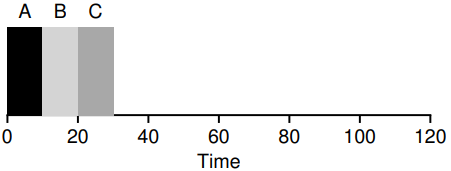
\includegraphics[width=\linewidth]{imgs/sched_fifo1}
\end{minipage}
\begin{minipage}{.5\linewidth}
short queued after long, bad
\begin{equation*}
  T_{\text{turnard}} = \frac{100+110+120}{3} = 110
\end{equation*}
\end{minipage}
\begin{minipage}{.5\linewidth}
  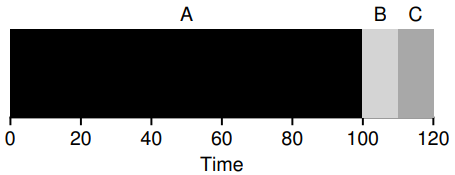
\includegraphics[width=\linewidth]{imgs/sched_fifo2}
\end{minipage}
% SJF
\begin{minipage}{.5\linewidth}
\section*{Shortest Job First (SJF)}
\begin{equation*}
  T_{\text{turnard}} = \frac{10+20+120}{3} = 50
\end{equation*}
\end{minipage}
\begin{minipage}{.5\linewidth}
  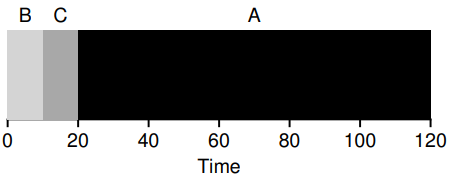
\includegraphics[width=\linewidth]{imgs/sched_fifo3}
\end{minipage}
\begin{minipage}{.5\linewidth}
  \begin{align*}
    & T_{\text{arrival-B}} = T_{\text{arrival-C}} = 10 \\
    & T_{t} = 103.33 = \\
    &\frac{100+(110-10)+(120-10)}{3} \\
  \end{align*}
\end{minipage}
\begin{minipage}{.5\linewidth}
  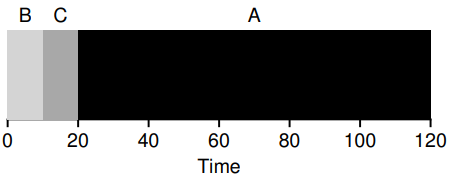
\includegraphics[width=\linewidth]{imgs/sched_fifo3}
\end{minipage}
\begin{minipage}{.5\linewidth}
  \begin{align*}
    & T_{t} = 50 = \\
    & \frac{(120-0)+(20-10)+(30-10)}{3} \\
  \end{align*}
\end{minipage}
\begin{minipage}{.5\linewidth}
  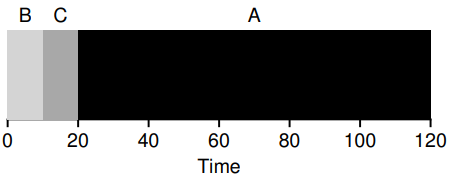
\includegraphics[width=\linewidth]{imgs/sched_fifo3}
\end{minipage}
\section*{Scheduling Metric 1: Response Time}
\begin{equation}
  \label{eq:reponse}
  T_{\text{response}} = T_{\text{firstrun}} - T_{\text{arrival}}
\end{equation}
\begin{minipage}{.5\linewidth}
  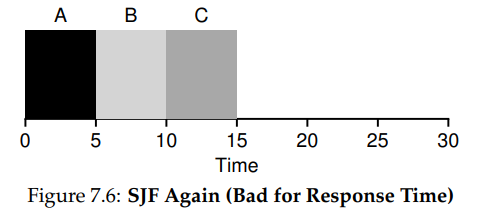
\includegraphics[width=\linewidth]{imgs/sched_rr1}
\end{minipage}
\begin{minipage}{.5\linewidth}
  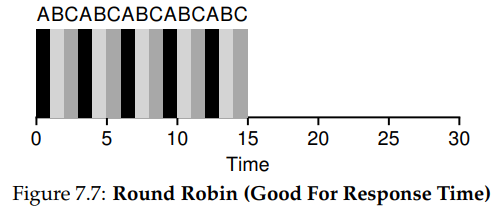
\includegraphics[width=\linewidth]{imgs/sched_rr}
\end{minipage}
\begin{minipage}{.5\linewidth}
  \centering
  SJF, $T_{r} = \frac{0+5+10}{3} = 5$
\end{minipage}
\begin{minipage}{.5\linewidth}
  RR (1s time slice), $T_{r} = \frac{0+1+2}{3} = 1$
\end{minipage}
\section*{Overlap improves resource usage}
\begin{minipage}{.45\linewidth}
  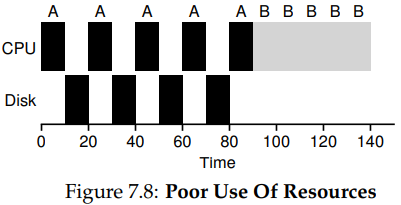
\includegraphics[width=\linewidth]{imgs/sched_io1}
\end{minipage}
\begin{minipage}{.55\linewidth}
  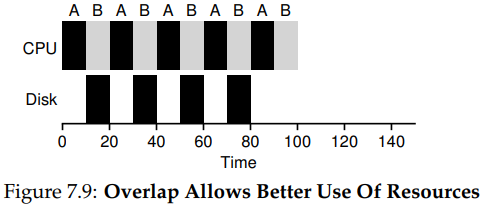
\includegraphics[width=\linewidth]{imgs/sched_io2}
\end{minipage}
\section*{MLFQ: Multi-Level Feedback Queue}
\begin{itemize}
\item \textbf{Rule 1}: if Priority(A) $>$ Priority(B), A runs (B doesn't)
\item \textbf{Rule 2}: if Priority(A) = Priority(B), A \& B runs in RR
\item \textbf{Rule 3}: When a job enters the system, it is placed at the \mo{highest} priority (the topmost queue)
\item \textbf{Rule 4}: Once a job uses up its time allotment at a given level (regardless of how many times it has given up the CPU), its priority is reduced (i.e., it moves down one queue)
\item \textbf{Rule 5}: After some time period S, move all the jobs in the system to the topmost queue.
\end{itemize}
\begin{minipage}{.4\linewidth}
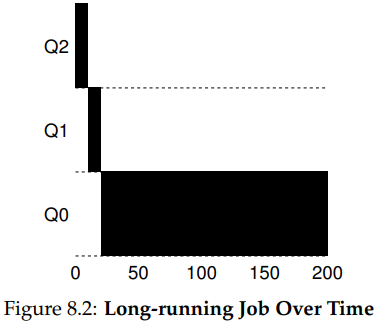
\includegraphics[width=\linewidth]{imgs/sched_longr}
\end{minipage}
\begin{minipage}{.6\linewidth}
  \flushleft
  \begin{itemize}
  \item assume time slice = 10 ms (with the allotment set equal to the time slice)
  \item the job enters at the highest priority (Q2)
  \item  After a single time slice of 10 ms, the scheduler reduces the job's priority by one, and thus the job is on Q1
  \item After running at Q1 for a time slice, the job is finally lowered to the lowest priority in the system (Q0), where it remains
  \end{itemize}
\end{minipage}
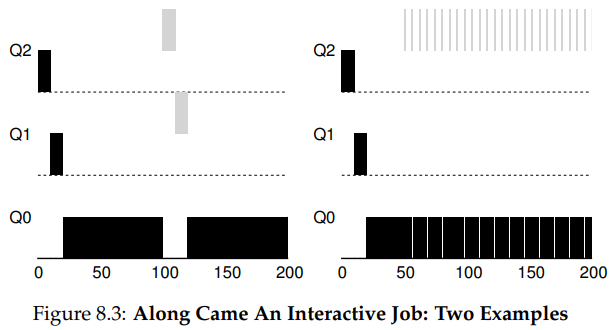
\includegraphics[width=\linewidth,height=3.5cm]{imgs/sched_long2}
\begin{minipage}{.5\linewidth}
  \flushleft
  \begin{itemize}
  \item  Job A (black) running along in the lowest-priority queue (as would any long-running CPU-intensive jobs)
  \item B (gray) arrives at time $T$ = 100; inserted into the highest queue
  \item B's short run-time: only 20 ms and completes before reaching the bottom queue in two time slices
  \item A resumes running (at low priority, as expected)
  \end{itemize}
\end{minipage}
\begin{minipage}{.5\linewidth}
  \flushleft
  \begin{itemize}
  \item interactive job B (gray) needs CPU only for 1ms before an I/O competing for CPU
  \item a long-running batch job A (shown in black)
  \item The MLFQ approach keeps B at the highest priority because B keeps releasing the CPU
  \item if B is an interactive job, MLFQ further achieves its goal of running interactive jobs quickly
  \end{itemize}
\end{minipage}
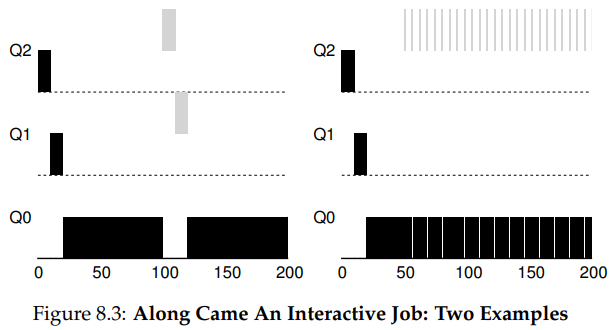
\includegraphics[width=\linewidth,height=3.5cm]{imgs/sched_long2}
\begin{minipage}{.5\linewidth}
  \flushleft
  \begin{itemize}
  \item there is no priority boost
  \item the long-running job gets starved once the two short jobs arrive
  \end{itemize}
\end{minipage}
\begin{minipage}{.5\linewidth}
  \flushleft
  \begin{itemize}
  \item there is a priority boost every 100ms (larger in real-world)
  \item long-running job gets boosted to the highest priority every 100ms
  \end{itemize}
\end{minipage}
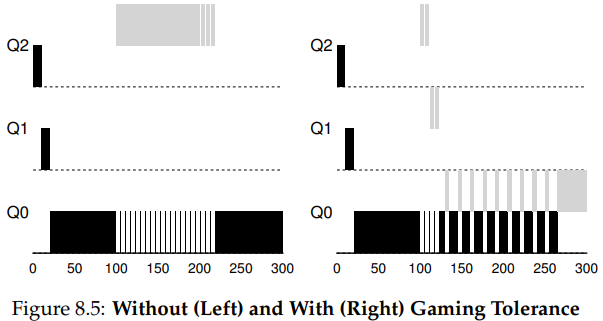
\includegraphics[width=\linewidth,height=3.5cm]{imgs/sched_g}
\begin{minipage}{.5\linewidth}
  \flushleft
  \begin{itemize}
  \item issue an I/O before proc's allotment ends $\to$ stay at same priority level; dominate CPU time
  \end{itemize}
\end{minipage}
\begin{minipage}{.5\linewidth}
  \flushleft
  \begin{itemize}
  \item regardless of the I/O behavior of proc, it slowly moves down the queues: \emph{cannot} dominate CPU
  \end{itemize}
\end{minipage}
\section*{Lottery Scheduler (need a random algorithm; has \emph{no} global state)}
\begin{minipage}{.75\linewidth}
\begin{lstlisting}[language=c]
// counter: used to track if we've found winner yet
int counter = 0;
// winner: call some random number generator to
// get a value >= 0 and <= (totaltickets - 1)
int winner = getrandom(0, totaltickets);
// current: use this to walk through the list of jobs
node_t *current = head; // best sorted HighT -> lowT
   while (current) {
   counter = counter + current->tickets;
   if (counter > winner)
      break; // found the winner
   current = current->next;
 }
 // `current' is the winner: schedule it...
\end{lstlisting}
\end{minipage}
\begin{minipage}{.25\linewidth}
  \flushleft
  \begin{itemize}
  \item probabilistic fairness, not deterministic
  \item scheduler must know total \# of tickets
  \item need data structs to track procs (e.g. list)
  \item for best efficiency, sort task-tickets from high to low
  \end{itemize}
\end{minipage}
\begin{minipage}{.45\linewidth}
  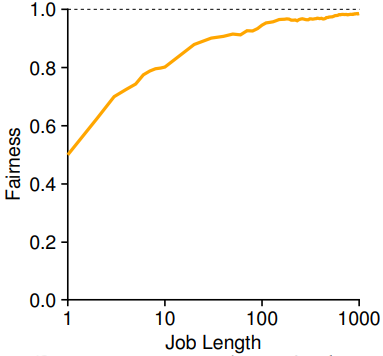
\includegraphics[width=\linewidth]{imgs/sched_lot_fair}
\end{minipage}
\begin{minipage}{.55\linewidth}
  \flushleft
  \begin{itemize}
  \item fairness metric $F = \frac{T_{\text{1st-job-done}}}{T_{\text{2nd-job-done}}}$
  \item for all jobs: same runtime $R$ and tickets (100)
  \item if $T_1 = 10$ $T_2 = 20$, $F = \frac{10}{20} = 0.5$
  \item if $T_1 = T_2 \to F = 1$, perfectly fair
  \item when job length not very long, average fairness quite low
  \item when jobs run for a significant number of time slices, lottery scheduler approach the desired fair outcome
  \end{itemize}
\end{minipage}
\section*{Linux Completely Fair Scheduler (CFS) and Weighting (Niceness)}
\begin{itemize}
\item goal: to fairly divide a CPU evenly among all competing processes
\item as each proc runs, \texttt{vruntime} $\uparrow$ at same rate, in proport.
with real time
\item when scheduling, CFS picks the proc with \mo{lowest} \texttt{vruntime} to run next
\item if CFS switch too often: fairness $\uparrow$, ctx switch cost $\uparrow$, performance $\downarrow$
\item CFS uses \texttt{sched\_latency} to decide length a proc runs before switch; typical 48ms and each proc runs 48/$n$ where $n=$ \# of procs
\item CFS uses \texttt{Min(sched\_latency, min\_granularity)} min defaults to 6ms to avoid large $n$ and tiny \texttt{sched\_latency} $\to$ close to 100\% fairness
\item CFS uses a \mo{periodic timer interrupt} $\to$ only make decisions at fixed time intervals (1ms); CFS tracks \texttt{vruntime} precisely: over the long haul, eventually approximate ideal sharing of the CPU
\end{itemize}
\begin{minipage}{.66\linewidth}
\begin{lstlisting}[language=c]
static const int prio_to_weight[40] = {
   /* -20 */ 88761, 71755, 56483, 46273, 36291,
   /* -15 */ 29154, 23254, 18705, 14949, 11916,
   /* -10 */ 9548, 7620, 6100, 4904, 3906,
   /*  -5  */ 3121, 2501, 1991, 1586, 1277,
   /*   0  */ 1024, 820, 655, 526, 423,
   /*   5  */ 335, 272, 215, 172, 137,
   /*  10  */ 110, 87, 70, 56, 45,
   /*  15  */ 36, 29, 23, 18, 15,
};
\end{lstlisting}
\end{minipage}
\begin{minipage}{.34\linewidth}
  \flushleft
  \begin{itemize}
  \item \mb{nice} level of a process $[-20, +19]$
  \item default nice = 0
  \item +nice $\to$ \mo{lower} priority
  \item -nice $\to$ \mo{higher} priority
  \item for each process: nice value \ding{220} \texttt{weight}
  \item preserves CPU proportion ratios
  \end{itemize}
\end{minipage}
\vspace{-.3em}
\begin{equation}
  \label{eq:timeslice}
  \texttt{time\_slice}_{k} = \frac{\texttt{weight}_{k}}{\sum_{i=0}^{n-1}\texttt{weight}_{i}}\cdot \texttt{sched\_latency}
\end{equation}
\begin{itemize}
\item jobs A (nice: -5) and B (nice: 0) $\to$ \texttt{weight}$_{A}$ = 3121; \texttt{weight}$_{B}$ = 1024
\item \texttt{time\_slice}$_{A} \approx \frac{3}{4}$ \texttt{sched\_latency} = 36ms; \texttt{time\_slice}$_{B} \approx 12$ms
\end{itemize}
\begin{equation}
  \label{eq:vruntime}
  \texttt{vruntime}_{i} = \texttt{vruntime}_{i} + \frac{\texttt{weight}_{0}}{\texttt{weight}_{i}}\cdot \texttt{runtime}_{i}
\end{equation}
\begin{itemize}
\item if nice$_{A}$ = 5, nice$_{B}$ = 10, CFS scheds them \emph{exactly} same as above
\item CFS uses a \ml{red}-black tree $O(\log(n))$: \emph{only} \mo{running} or \mo{runnable} procs kept therein; sleeping proc removed from the tree, tracked elsewhere
\item a job wakes, its \texttt{vruntime} sets to min value in the tree: no starvation
\item CFS can schedule across large groups of procs, not just individuals
\end{itemize}

% \section*{Memory (compiled and runnable \texttt{!=} correct)}
\begin{tabular}[th!]{l|ccc}
  \hline
  type & allocation & deallocation & life cycle \\
  \hline
  stack* & implicit (compiler) & implicit (compiler) & short \\
  heap & explicit (user) & explicit (user) & long \\
  \hline
  \multicolumn{3}{l}{*: also called \textbf{automatic} memory}\\
  \hline
\end{tabular}
\begin{tabular}[th!]{l|lp{6.5cm}}
  \hline
  name & type & usage \\
  \hline
  \texttt{malloc} & lib call & dynamic memory alloc without zeroing \\
  \texttt{calloc} & lib call & dynamic memory alloc with zeroing\\
  \texttt{realloc} & lib call & dynamic memory allocation \\
  \texttt{free} & lib call & only accepts memory alloced by \texttt{re/malloc} \\
  \texttt{brk} & sys call & sets program break to specific value; user programs should avoid using it directly \\
  \texttt{sbrk} & sys call & increment program break by n bytes; user programs should avoid using it directly \\
  \texttt{mmap} & sys call & commonly used by allocator, not by user programs \\
  \hline
\end{tabular}
\begin{itemize}
\item idiom for string: \texttt{malloc(strlen(s) + 1)}
\item the size of allocated region \emph{must} be tracked by memory-allocator itself
\end{itemize}
\section*{Common memory errors}
\begin{enumerate}
\item Forget to Allocate Memory
  \begin{lstlisting}[language=c,xrightmargin=2pt]
char *src = "hello";
char *dst; // oops! unallocated; (char *) malloc(5 * sizeof char)
strcpy(dst, src); // segfault
\end{lstlisting}

\item Not Allocate Enough Memory (buffer overflow)
\begin{lstlisting}[language=c,xrightmargin=2pt]
char *src = "hello";
char *dst = (char *) malloc(strlen(src)); // too small!
strcpy(dst, src); // may work properly
\end{lstlisting}

\item Forget to Initialize Allocated Memory
  \begin{itemize}
  \item Will eventually encounter an uninitialized read (undefined behavior)
  \item Out-of-bound read/write
  \end{itemize}

\item Forget to Free Memory (memory leak)
  \begin{itemize}
  \item In long-running apps or systems (such as OS itself), slowly leaking memory eventually results in running out of memory
  \item For short-lived, soon-exiting programs, OS will clean up, thus \emph{no} memory leak (bad habit anyway)
  \end{itemize}

\item Use-after-free (dangling pointer)
\item Free Memory Repeatedly (double free)
\item Call \texttt{free()} Incorrectly (invalid free)
  \begin{itemize}
  \item Freeing an uninitialized/arbitrary pointer
  \item Freeing the wrong pointer or freeing NULL pointer
  \end{itemize}
\end{enumerate}
\subsection*{Two levels of memory management in system}

\begin{enumerate}
\item performed by the OS, which hands out memory to processes when they run, and takes it back when processes exit (or otherwise die)
\item \emph{within} each process, e.g. when calling \texttt{malloc()} or \texttt{free()}.  OS will reclaim \emph{all} the memory of the process (including those pages for code, stack and heap) when program is finished running. No matter what the state of your heap in your address space, the OS takes back all of those pages when the process dies, thus ensuring that no memory is lost despite the fact that you didn’t free it.
\end{enumerate}
\subsection*{Reasons for dynamic memory}
\begin{itemize}
\item the amount of required memory may be task dependent
\item input size may be unknown at compile time
\item conservative pre-allocation would be wasteful
\item recursive functions
\end{itemize}

% \section*{Goals of Virtual Memory (VM) system}
\begin{enumerate}
\item \textbf{transparency} invisible to running prog (illusion: private ph. mem)
\item \textbf{efficiency} OS needs hardware support (e.g. TLBs)
  \begin{itemize}
  \item time (not making programs run much more slowly)
  \item space (not using too much mem for structs to support virtualization)
  \end{itemize}
\item \textbf{protection} thus enables isolation among processes
\end{enumerate}
\section*{Address Translation (hardware-based)}
\begin{minipage}{\linewidth}
  \centering
  \texttt{physical address = virtual address + base}
\end{minipage}
\begin{minipage}{0.45\linewidth}
  \begin{enumerate}
  \item Each memory reference by a process is a virtual address
  \item isolation property is satisfied (security)
  \item translation and check are cheap (performance)
  \end{enumerate}
\end{minipage}
\begin{minipage}{.5\linewidth}
  \begin{lstlisting}[language=c,xleftmargin=2pt]
if (addr < bounds)
  return *(base + addr);
else
  throw new SegFaultException;
// Waste physical mem (must alloc all)
// No (easy) sharing btw procs
\end{lstlisting}
\end{minipage}

\section*{Dynamic Relocation: Hardware Requirements}
\begin{tabular}[th!]{p{3.5cm}p{5.4cm}}
  Hardware Requirements & Notes \\
  \hline
  Privileged mode & Needed to prevent user-mode processes from executing privileged operations \\
  \hline
  Base/bounds registers & Need pair of registers per CPU to support address translation and bounds checks \\
  \hline
  Able to translate virtual addr and check bounds & Circuitry to do translations and check limits; in this case, quite simple\\
  \hline
  Privileged instructions to update base/bounds & OS must be ablt to set these values before letting a user program run \\
  \hline
  Privileged instructions to register exception handlers & OS must be able to tell hardware what code to run if exception occurs \\
  \hline
  Able to raise exceptions & When processes try to access privileged instructions or out-of-bounds memory \\
  \hline
\end{tabular}
\section*{Hardware support in base/bounds virtual memory}
\begin{enumerate}
\item provide 2 different CPU modes
  \begin{itemize}
  \item privileged mode (kernel mode) to access entire machine
  \item user mode (limited direction execution)
  \item a single bit stored in processor status word indicating current mode
  \end{itemize}
\item provide base and bounds registers (MMU)
\item provide \textbf{privileged} instructions to modify the base/bounds registers
\item provide exception handler to handle exceptions generated by CPU
  \begin{itemize}
  \item CPU should stop executing user program and raise exception
  \item CPU should be able to inform OS of handlers location (privileged)
  \end{itemize}
\end{enumerate}
\section*{Dynamic Relocation: Hardware Requirements}
\begin{tabular}[th!]{p{3cm}p{6cm}}
  OS Requirements & Notes \\
  \hline
  Memory management & \parbox[t]{6cm}{Need to allocate memory for new processes\\
  Reclaim memory from terminated processes \\
  Generally manage memory via \textbf{free list}} \\
  \hline
  Base/bounds management & Must set base/bounds properly on context switch\\
  \hline
  Exception handling  & \parbox[t]{6cm}{Code to run when exception arise\\
  liley action is to terminate offending process} \\
  \hline
\end{tabular}
\section*{OS support in base/bounds virtual memory}
\begin{enumerate}
\item when a process is created, finding space for its addr space in memory
\item when a process is terminated (exits gracefully or forcefully killed), reclaiming all of its memory (putting back to free list).
\item when a context switch occurs, performing a few additional steps: save and restore base-and-bounds pair to memory in process structure or process control block (PCB)
\item must provide exception handlers
\end{enumerate}

% \section*{Segmentation: Generalized Base/bounds}
\begin{minipage}{.6\linewidth}
  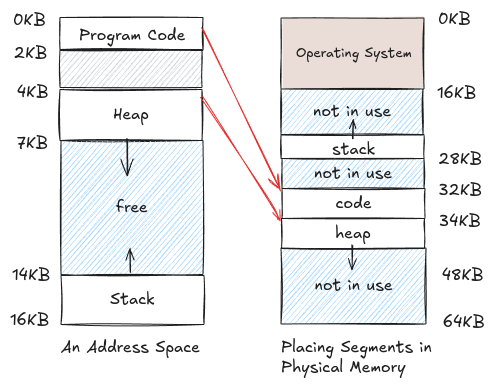
\includegraphics[width=\linewidth]{imgs/addr_map}
\end{minipage}
\begin{minipage}{.4\linewidth}
  \begin{tabular}[th!]{lccl}
    Seg. & Base & Size & Offset\\
    \hline
    Code & 32K  & 2K   & 0     \\
    Heap & 34K  & 3K   & 4K    \\
    Stak & 28K  & 2K   & 16K*   \\
    \hline
    \multicolumn{4}{l}{* stack grows to lower addr} \\
    \hline
  \end{tabular}
  Given addr in the segment:\\
  new = addr \textcolor{err}{-} offset + base
  \begin{itemize}
  \item Addr 100 in code segment:
  \item[] 100 - 0 + 32K = 32868
  \item Addr 4200 in heap segment:
  \item[] 4200 - 4K + 32K = 34920
  \item Addr 7100 $\to$ seg. fault
  \end{itemize}
\end{minipage}
\section*{Segment Reference (explicit approach)}
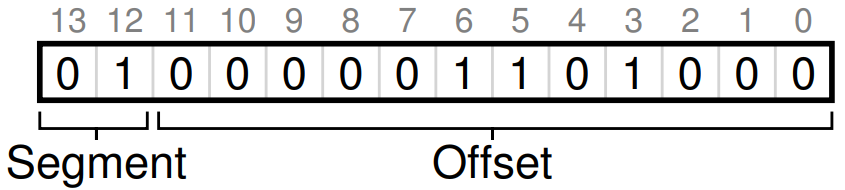
\includegraphics[width=\linewidth]{imgs/explicit2}
\begin{itemize}
\item one segment is unused $\to$ put code in heap to use 1 bit for segment
\item virtual address space is limited to 4KB (max in this example)
\end{itemize}
\section*{Stack and Sharing}
\begin{tabular}[th!]{lcclll}
  Seg. & Base & Size (max 4K) & Offset & Grows pos? & Protection*\\
  \hline
  Code$_{00}$ & 32K  & 2K   & 0    & 1 & Read-Exec  \\
  Heap$_{01}$ & 34K  & 3K   & 4K   & 1 & Read-Write \\
  Stak$_{11}$ & 28K  & 2K   & 16K  & 0 & Read-Write \\
  \hline
  \multicolumn{6}{l}{* protection bits in hardware is to support code sharing} \\
  \hline
\end{tabular}
Virtual addr: 11 1100 0000 0000 $\to$ 15K (0x3c00)
\begin{itemize}
\item 11 $\to$ in stack segment and left 3K (1100 0000 0000)
\item mapped = 3K - 4K (max segment size) + 28K (base) = 27K
\end{itemize}

% \section*{Arithmetics in Paging (Size, Page Numbers, PTE numbers)}
\begin{minipage}{0.55\linewidth}
  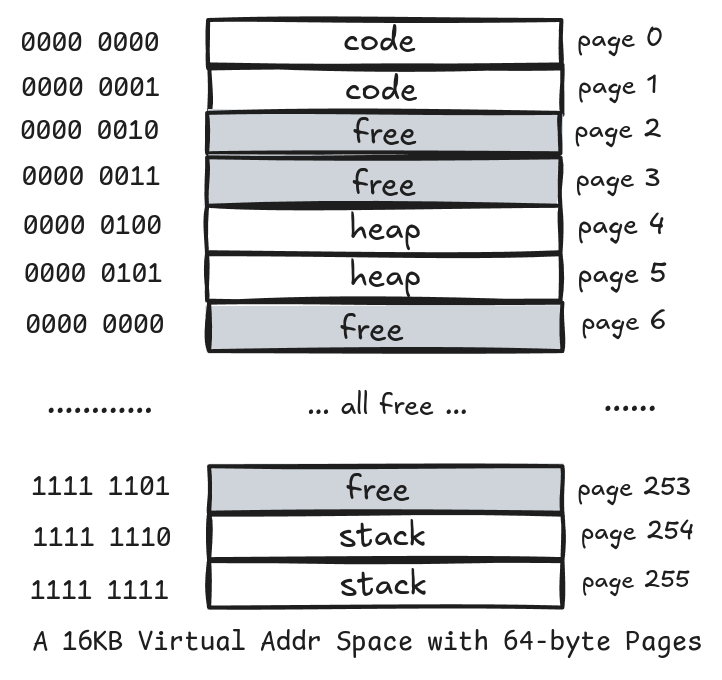
\includegraphics[width=\linewidth]{imgs/virtual_addr_eg}
  \flushleft
  \begin{itemize}
  \item $S_{\text{AS}}$ = 16KB = $16 \times 1024 = 2^{4} \times 2^{10} = 2 ^{14}$B
  \item V Addr bit width = $\log_2 S_{\text{AP}} = 14$
  \item $S_{\text{P}}$ = 64B = $2^{6}$B
  \item \textbf{Offset} bit width = $\log_2 S_{\text{P}} = 6$
  \item VPN bit width = 14 - 6 = 8
  \item $N_{\text{P}}$ = $\frac{S_{\text{AS}}}{S_{\text{P}}} = \frac{2^{14}}{2^{6}} = 2^{8}$
  \item $N_{\text{PTE}} = N_{\text{P}} = 2^{8} = 256$ (linear PT)
  \end{itemize}
\end{minipage}
\begin{minipage}{0.45\linewidth}
  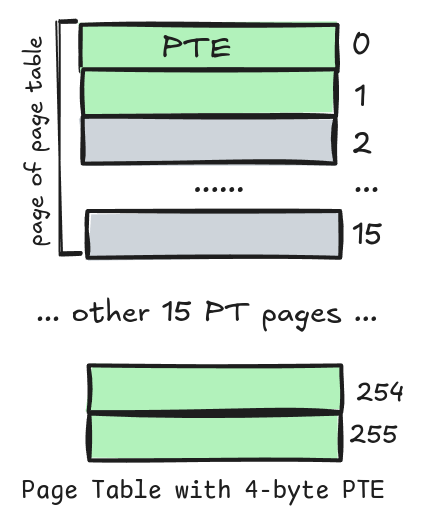
\includegraphics[width=\linewidth]{imgs/pte_4byte}
  \flushleft
  \begin{itemize}
  \item $S_{\text{PTE}} =4$B
  \item $S_{\text{PT}} = N_{\text{PTE}} \times S_{\text{PTE}} = 1\text{KB} $
  \item Page table can be divided into pages (for 2-level PT)
  \item[] $S_{\text{PTP}} = \frac{S_{\text{PT}}}{S_{\text{P}}} = \frac{1024}{64} = 16$
  \item Each PDE points to a PTP of 16 PTEs
  \end{itemize}
\end{minipage}


% \pagebreak
% \section*{Paging: Two Advantages and Address Translation}
\begin{enumerate}
\item \textbf{flexibility}: support abstraction of address space: no need to assume direction of stack/heap growth and how they are used
\item \textbf{simplicity}: easy to manage free space: simply keep a list of free pages
\end{enumerate}
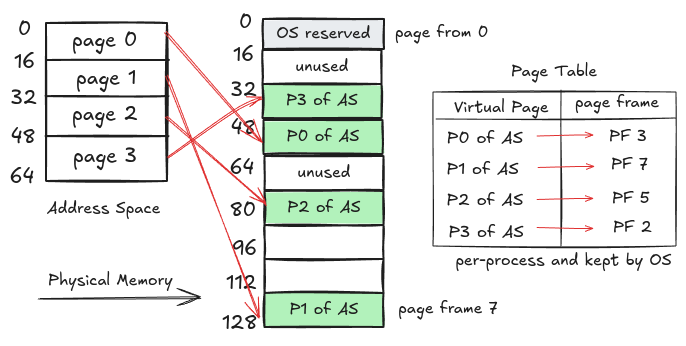
\includegraphics[width=\linewidth,height=4.5cm]{imgs/page_table}
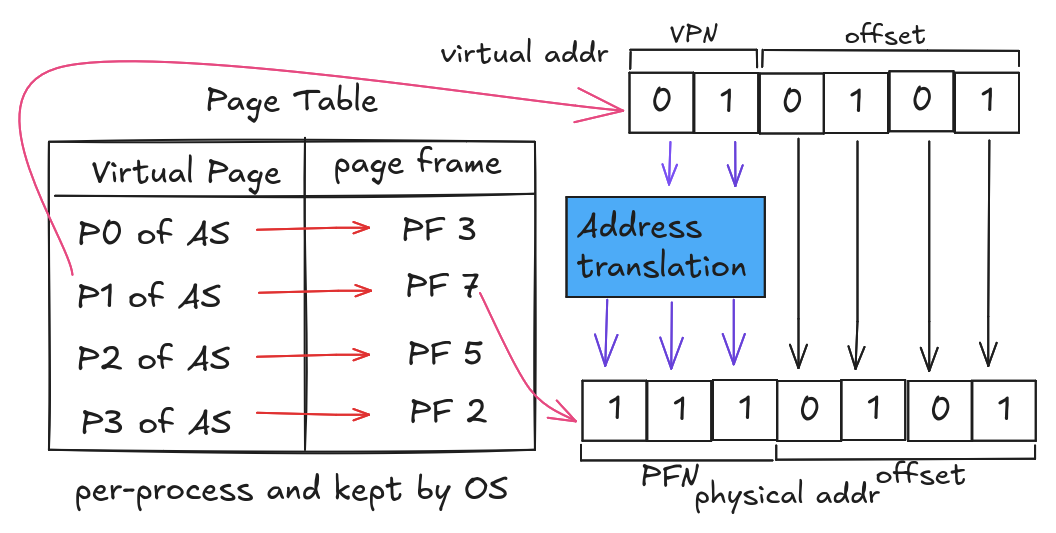
\includegraphics[width=\linewidth,height=4cm]{imgs/address_trans}
\section*{Page Table Issues: too big and too slow}
\begin{minipage}{0.5\linewidth}
  \flushleft
  \begin{itemize}
  \item 32-bit addr space, 4K pages: 20-bit VPN, 12-bit offset
  \item $2^{20} \approx 1$ million entries in page table for 1 process
  \item Assume each \textbf{PTE} needs 4B, 1 proc needs 4MB page table!
  \item Too big for MMU: physical memory or disk (by swapping page frams in/out of mem to disk)
  \end{itemize}
\end{minipage}
\begin{minipage}{0.5\linewidth}
  \begin{itemize}
  \item Extract VPN from virtual addr (VA) to find PFN
  \item Locate page table (e.g. in a page-table reg.)
  \item Compute addr of PTE for VPN
  \item Extract offset from VA and compute physical addr (PA)
  \item Fetch data from memory at PA
  \end{itemize}
\end{minipage}
\section*{Page Table Entry (PTE)}
Each PTE needs to store target PFN plus a few more information:
\begin{itemize}
\item valid bit: whether the VPN is mapped or not
\item protection bits: whether page is for read/write/code-execution
\item present bit: whether page is in memory or disk (swapped out)
\item dirty bit: page modified since it's brought to memory (swapping on)
\item reference bit: page has been accessed; for policies for page replacement
\end{itemize}
\section*{Accessing Memory With Paging}
\begin{lstlisting}[language=c]
VPN = (VirtualAddr & VPN_MASK) >> SHIFT    // get VPN from VA
PTEAddr = PTBR + (VPN * sizeof(PTE))        // compute PET addr
PTE = AccessMemory(PTEAddr)                 // fetch PTE
// Check if process can access the page
if (PTE.Valid == False)
  RaiseException(SEGMENTATION_FAULT)
else if (CanAccess(PTE.ProtectBits) == False)
  RaiseException(PROTECTION_FAULT)
else
  offset = VirtualAddress & OFFSET_MASK           // access ok
  PhysAddr = (PTE.PFN << PFN_SHIFT) | offset      // form physical addr
  Register = AccessMemory(PhysAddr)               // fetch it
\end{lstlisting}

% \columnbreak
% \section*{TLB (faster translation)}
TLB performance (cache perf. in general) improved by two factors:
\begin{enumerate}
\item Spatial locality:  if a program accesses memory at address x , it
will likely soon access memory near x
\item Temporal locality:  ix recently accessed will likely be accessed soon
\end{enumerate}
\section*{TLB Control Flow Algorithm}
\begin{minipage}{.66\linewidth}
\begin{lstlisting}[language=c]
VPN = (VirtualAddr & VPN_MASK) >> SHIFT
(Success, TlbEntry) = TLB_Lookup(VPN)
if (Success == True) // TLB Hit
  if (CanAccess(TlbEntry.ProtectBits) == True)
    Offset = VirtualAddr & OFFSET_MASK
    PhysAddr = (TlbEntry.PFN << SHIFT) | Offset
    Register = AccessMemory(PhysAddr)
  else
    RaiseException(PROTECTION_FAULT)
else // TLB Miss
  PTEAddr = PTBR + (VPN * sizeof(PTE))
  PTE = AccessMemory(PTEAddr)
  if (PTE.Valid == False)
    RaiseException(SEGMENTATION_FAULT)
  else if (CanAccess(PTE.ProtectBits) == False)
    RaiseException(PROTECTION_FAULT)
  else
    TLB_Insert(VPN, PTE.PFN, PTE.ProtectBits)
    RetryInstruction()
\end{lstlisting}
\begin{lstlisting}[language=c]
VPN = (VirtualAddr & VPN_MASK) >> SHIFT
(Success, TlbEntry) = TLB_Lookup(VPN)
if (Success == True) // TLB Hit
  if (CanAccess(TlbEntry.ProtectBits) == True)
    Offset = VirtualAddr & OFFSET_MASK
    PhysAddr = (TlbEntry.PFN << SHIFT) | Offset
    Register = AccessMemory(PhysAddr)
  else
    RaiseException(PROTECTION_FAULT)
  else // TLB Miss
    RaiseException(TLB_MISS)
\end{lstlisting}
\end{minipage}
\begin{minipage}{.34\linewidth}
  \flushleft
  \begin{itemize}
  \item CISC TLB miss $\to$HW
    \begin{enumerate}
    \item page table register stored in memory
    \item walk page table, find correct PTE, extract translation
    \item update TLB with the translation
    \item retry the instruction
    \end{enumerate}
  \item RISC TLB miss $\to$OS
    \begin{enumerate}
    \item hardware raises exception$\to$pause
    \item kernel mode$\to$trap
    \item OS updates TLB; returns from trap
    \end{enumerate}
  \item accessing large num of pages, exceeding \textbf{TLB} \textbf{coverage} in a short time $\to$ lots TLB miss
  \item TLB can be \textbf{bottleneck} in CPU pipeline, esp. with physically-indexed cache, because addr trans has to happen \emph{before} cache is accessed

  \end{itemize}
\end{minipage}
\section*{TLB Control Flow Algorithm (OS Handled)}
\begin{itemize}
\item when returning from a TLB miss-handling trap, hardware must resume execution at the ix that caused the trap, resulting in a TLB hit
\item OS must not cause infinite chain of TLB misses to occur
  \begin{enumerate}
  \item keep TLB miss handlers in physical mem (unmapped, no addr trans)
  \item reserve entries in TLB for permanently-valid trans and handler code itself (these wired translations always TLB hit)
  \end{enumerate}
\end{itemize}
\section*{TLB Entries (hardware search all entries for a match)}
\begin{minipage}{.45\linewidth}
  \flushleft
  \begin{enumerate}
  \item typically small (32/64/128 entries)
  \item \textbf{not} indexed by VPN
  \item \textbf{fully associative}
  \end{enumerate}
\end{minipage}
\begin{minipage}{.55\linewidth}
  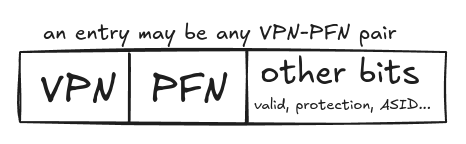
\includegraphics[width=\linewidth]{imgs/tlb_entry}
\end{minipage}
\section*{TLB: Context Switch}
\begin{minipage}{.45\linewidth}
  \flushleft
  \begin{enumerate}
  \item \textbf{flush} all entries
    \begin{itemize}
    \item whenever a proc resumes $\to$ TLB misses
    \item if ctx switch too frequently $to$ too costly
    \end{itemize}
  \end{enumerate}
\end{minipage}
\begin{minipage}{.55\linewidth}
  \begin{tabular}{ccccc}
    VPN & PFN & valid & prot & ASID \\
    \hline
    10 & 100  &   1   & rws  & 1    \\
    -  &  -   &   -   & -    & -    \\
    10 & 170  &   1   & rwx  & 2    \\
    \hline
  \end{tabular}
\end{minipage}
\begin{enumerate}
\item[2.] addr space identifier (ASID) to each TLB entry
  \begin{itemize}
  \item each proc with unique ASID
  \item entries contain different procs at same time while keep isolation
  \end{itemize}
\end{enumerate}
\section*{TLB: Replacement Policy (minimize miss rate or inc hit rate)}
\begin{enumerate}
\item replace \textbf{least-recently-used} (LRU)
\item evict a \textbf{random} entry
\end{enumerate}

% \section*{Hybrid: 3 (smaller) page tables per process}
\begin{minipage}{0.5\linewidth}
  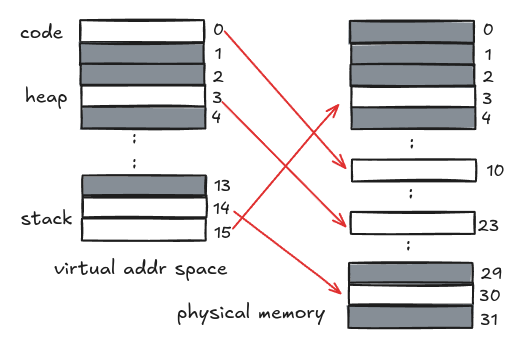
\includegraphics[width=\linewidth]{imgs/bigger_sparse_page}
\end{minipage}
\begin{minipage}{0.5\linewidth}
  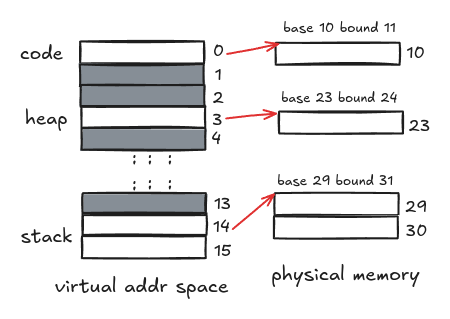
\includegraphics[width=\linewidth]{imgs/hybrid_page_table}
\end{minipage}
\begin{itemize}
\item each proc has \emph{three} associated page tables (right) instead of one (left)
\item each logical seg has 3 pairs of base/bound (hardware) regs: base points to the page table addr; bound shows page table size
\item use 2 bits for segment (e.g. 00 unused, 01 code, 10 heap, 11 stack)
\end{itemize}
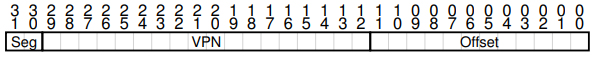
\includegraphics[width=\linewidth]{imgs/virtual_addr2_32big_hybrid}
\begin{minipage}{0.61\linewidth}
\begin{lstlisting}[language=c,xrightmargin=2pt]
SN = (VirtualAddr & SEG_MASK) >> SN_SHIFT
VPN = (VirtualAddr & VPN_MASK) >> VPN_SHIFT
AddrOfPTE = Base[SN] + (VPN * sizeof(PTE))
\end{lstlisting}
\end{minipage}
\begin{minipage}{0.39\linewidth}
  \flushleft
  \begin{itemize}
  \item \emph{bound} reg to decide how many pages to map
  \item SN (seg num) to decide which base/bound pair
  \end{itemize}
\end{minipage}
\begin{itemize}
\item not flexible: segmentations still assume usage patterns (separation of code/stack/heap in allocating pages)
\item \textbf{external fragmentation} While most of memory is managed in page-sized units, page tables now of arbitrary size (in multiples of PTEs). Thus, finding free space for them in memory is more complicated
\end{itemize}

% \section*{2-level page tables (smaller but slower)}
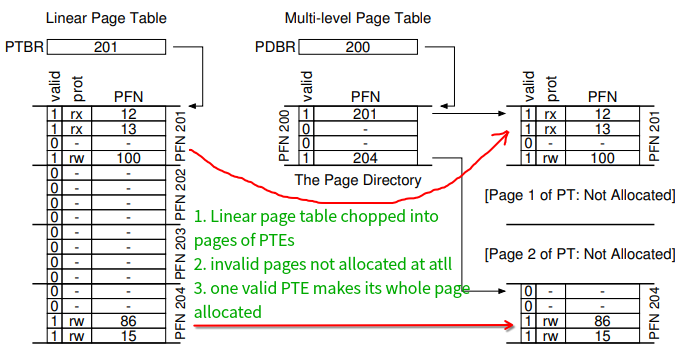
\includegraphics[width=\linewidth]{imgs/multi_level_pt}
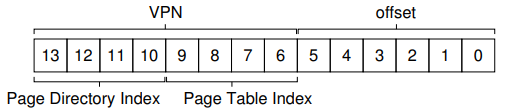
\includegraphics[width=\linewidth]{imgs/two_level_pt}
\begin{enumerate}
\item \texttt{PDEAddr = PageDirBase + (PDIndex * sizeof(PDE))}
\item \texttt{PTEAddr = PDE.PFN << SHIFT + (PTIndex * sizeof(PTE))}
\item \texttt{PhysAddr = (PTE.PFN << SHIFT) + offset}
\end{enumerate}
\begin{minipage}{.5\linewidth}
  \flushleft
  \begin{itemize}
  \item Space usage in proportion to in-use addr space
  \item carefully constructed, each portion of PT fits neatly within a page, \textbf{easier} memory management: OS grabs next free page for alloc or grow
  \end{itemize}
\end{minipage}
\begin{minipage}{.5\linewidth}
  \flushleft
  \begin{itemize}
  \item on TLB miss $\to$ two loads from memory (slower)
  \item increased \textbf{complexity} (hardware or OS) of handling page-table lookup (on TLB miss).
  \end{itemize}
\end{minipage}

% \section*{Multi-level ($\geq 2$) page table: an example}
\begin{tabular}{lllll}
  \hline
  VA bit & VA page size & Offset bit & PTE size & PDE size \\
  \hline
  30           & 512 byte     & $log_2 512 = 9$ & 4 byte & 4 byte \\
  \hline
\end{tabular}

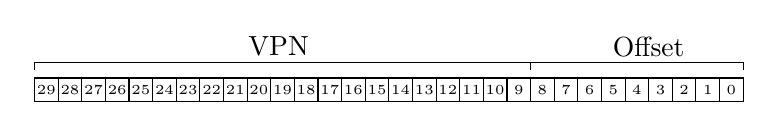
\begin{tikzpicture}
  % VPN
  \node at (3.1,0.7) (vpn){VPN};
  \draw (0, 0.4) -- (0,0.5);
  \draw (6.3, 0.4) -- (6.3,0.5);
  \draw (0, 0.5) -- (6.3,0.5);

  % Offset
  \node at (7.8,0.7) (off){Offset};
  \draw (6.3, 0.4) -- (6.3,0.5);
  \draw (9, 0.4) -- (9,0.5);
  \draw (6.3, 0.5) -- (9,0.5);

  \foreach \x [count=\xi from 0, evaluate=\xi as \num using int(29-\xi)] in
  {0,0.3,0.6,...,9}
  {
    \draw (\x, 0) rectangle (\x+0.3, 0.3);
    \node[font=\tiny] at (\x+0.15, 0.15) {\num};
  }
\end{tikzpicture}
\begin{itemize}
\item When chopping page table into pages, page table pages (PTP) usually have same \textbf{size} as virtual addr page: $S_{\text{VAP}} = S_{\text{PTP}} = 512$ bytes
\item Thus, each PTP will have $N_{\text{PTE}} = \frac{S_{\text{PTP}}}{S_{\text{PTE}}} = \frac{512}{4} = 128$ PTEs
\item To find each PTE, \texttt{PTIndex} need bits of $\log_2 N_{\text{PTE}} = \log_2 128 = 7$
\item The left 14 bits (30 - offset - \texttt{PTIndex}) used for Page Directory Index
\end{itemize}
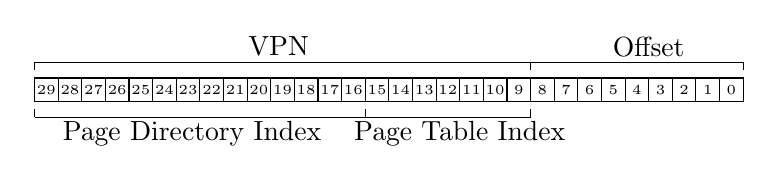
\begin{tikzpicture}
  % VPN
  \node at (3.1,0.7) (vpn){VPN};
  \draw (0, 0.4) -- (0,0.5);
  \draw (6.3, 0.4) -- (6.3,0.5);
  \draw (0, 0.5) -- (6.3,0.5);

  % Offset
  \node at (7.8,0.7) (off){Offset};
  \draw (6.3, 0.4) -- (6.3,0.5);
  \draw (9, 0.4) -- (9,0.5);
  \draw (6.3, 0.5) -- (9,0.5);

  \foreach \x [count=\xi from 0, evaluate=\xi as \num using int(29-\xi)] in
  {0,0.3,0.6,...,9}
  {
    \draw (\x, 0) rectangle (\x+0.3, 0.3);
    \node[font=\tiny] at (\x+0.15, 0.15) {\num};
  }

  % PDIndex
  \draw (0, -0.1) -- (0,-0.2);
  \draw (4.2, -0.1) -- (4.2,-0.2);
  \draw (0, -0.2) -- (4.2,-0.2);
  \node at (2,-0.4) (pdindex){Page Directory Index};

  % PTIndex
  \draw (4.2, -0.1) -- (4.2,-0.2);
  \draw (6.3, -0.1) -- (6.3,-0.2);
  \draw (4.2, -0.2) -- (6.3,-0.2);
  \node at (5.4,-0.4) (ptindex){Page Table Index};
\end{tikzpicture}
\begin{itemize}
\item this results in a \textbf{HUGE} PD itself: $2^{14}$ PEDs and requires 128 pages
\end{itemize}
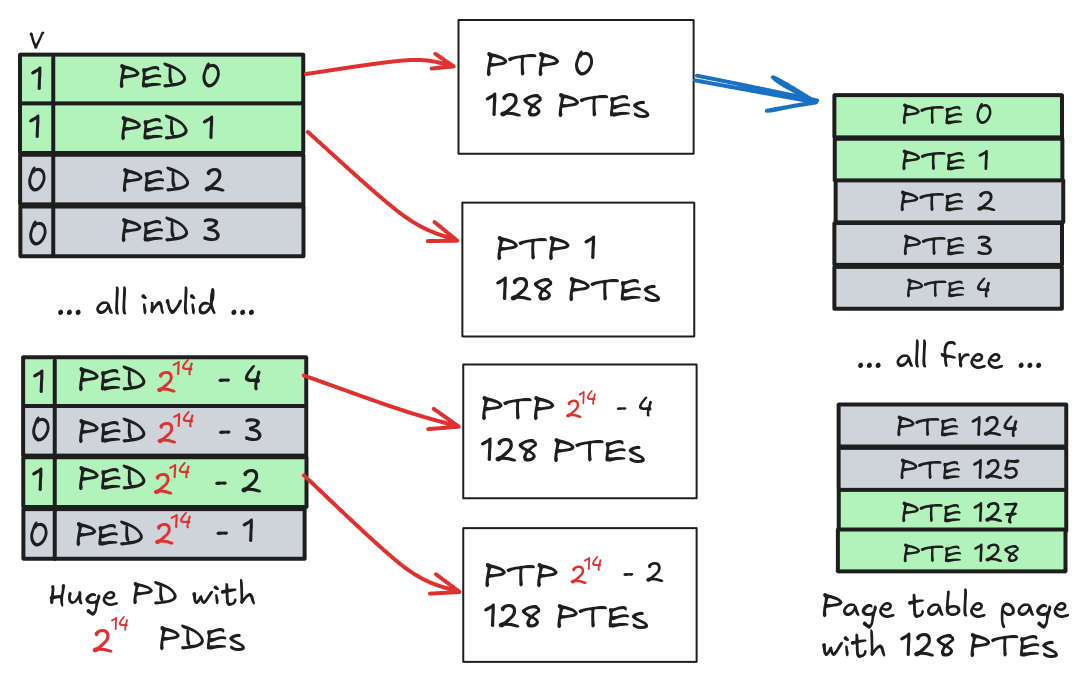
\includegraphics[width=\linewidth]{imgs/huge_2level_pt}
\begin{itemize}
\item Splitting PD into 2 levels and each level has same bit width: 7
\item TLB miss causes additional memory accesses
\end{itemize}
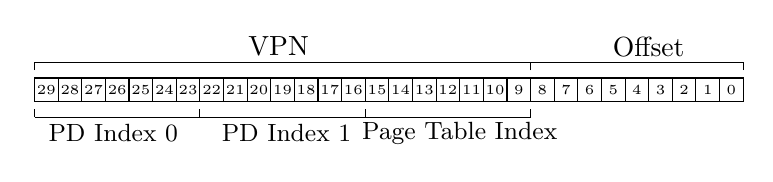
\begin{tikzpicture}
  % VPN
  \node at (3.1,0.7) (vpn){VPN};
  \draw (0, 0.4) -- (0,0.5);
  \draw (6.3, 0.4) -- (6.3,0.5);
  \draw (0, 0.5) -- (6.3,0.5);

  % Offset
  \node at (7.8,0.7) (off){Offset};
  \draw (6.3, 0.4) -- (6.3,0.5);
  \draw (9, 0.4) -- (9,0.5);
  \draw (6.3, 0.5) -- (9,0.5);

  \foreach \x [count=\xi from 0, evaluate=\xi as \num using int(29-\xi)] in
  {0,0.3,0.6,...,9}
  {
    \draw (\x, 0) rectangle (\x+0.3, 0.3);
    \node[font=\tiny] at (\x+0.15, 0.15) {\num};
  }

  % PDIndex 0
  \draw (0,   -0.1) -- (0,  -0.2);
  \draw (2.1, -0.1) -- (2.1,-0.2);
  \draw (0,   -0.2) -- (2.1,-0.2);
  \node at (1,-0.4) (pdindex0){\small PD Index 0};

  % PDIndex 1
  \draw (4.2, -0.1) -- (4.2,-0.2);
  \draw (2.1, -0.2) -- (4.2,-0.2);
  \node at (3.2,-0.4) (pdindex1){\small PD Index 1};

  % PTIndex 0
  \draw (4.2, -0.1) -- (4.2,-0.2);
  \draw (6.3, -0.1) -- (6.3,-0.2);
  \draw (4.2, -0.2) -- (6.3,-0.2);
  \node at (5.4,-0.4) (ptindex){\small Page Table Index};
\end{tikzpicture}

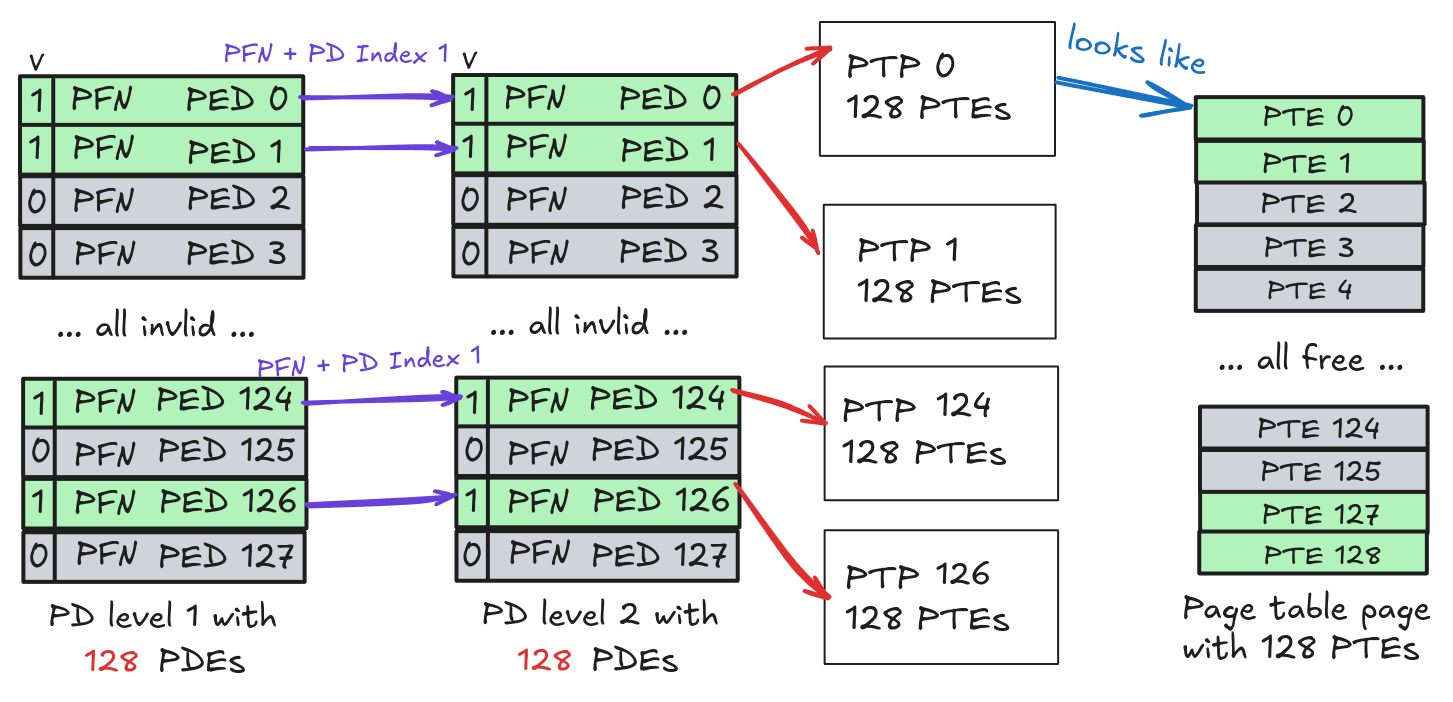
\includegraphics[width=\linewidth]{imgs/smaller_3level_pt}

\begin{itemize}
\item the bigger the page table, the faster a TLB miss can be serviced
\item memory-constrained (old) system, smaller page tables preferred
\end{itemize}

% \section*{Swapping (transparent to process)}
\begin{itemize}
\item For more than avail. physical memory $\to$ use 2nd storage, SSD etc.
\item Space on disk reserved to move pages back/forth to memory
\item OS reads/writes to swap space in \textbf{page-sized} units
\item OS needs to remember disk address of a given page
\item TLB uses this bit to track if a page is present in physical memory
\end{itemize}
\section*{Why hardware doesn't handle page faults}
\begin{enumerate}
\item page faults to disk are \emph{slow}; extra overheads of software are minimal
\item the hardware would have to understand swap space, how to issue I/Os to disk, and lots other details it currently doesn't know much about
\end{enumerate}
\section*{OS handles page faults via swapping}
while I/O is in flight, process will be in blocked state. Thus, OS will be free to run other ready processes while page fault is being serviced
\begin{enumerate}
\item page tables stores bits info about where to find the desired page
\item OS uses the bits in PTE for a disk address
\item On page fault, OS looks in PTE to find the address and issues request to disk to fetch page into memory
\item When disk I/O done, OS marks the page in PT as present, update PFN field of PTE to record in-memory location of newly-fetched page, and retry ix
\item This next attempt may cause TLB miss which would then be serviced and update TLB with addr translation (or update TLB directly)
\item a last restart would find the translation in TLB and proceed to fetch desired data/instruction from memory at translated physical address
\end{enumerate}
\section*{Page-Fault Control Flow Algorithm (Hardware)}
\begin{minipage}{.72\linewidth}
\begin{lstlisting}[language=c]
VPN = (VirtualAddress & VPN_MASK) >> SHIFT
(Success, TlbEntry) = TLB_Lookup(VPN)
if (Success == True) // TLB Hit
   if (CanAccess(TlbEntry.ProtectBits) == True)
      Offset = VirtualAddress & OFFSET_MASK
      PhysAddr = (TlbEntry.PFN << SHIFT) | Offset
      Register = AccessMemory(PhysAddr)
   else
      RaiseException(PROTECTION_FAULT)
else                 // TLB Miss
   PTEAddr = PTBR + (VPN * sizeof(PTE))
   PTE = AccessMemory(PTEAddr)
   if (PTE.Valid == False)
      RaiseException(SEGMENTATION_FAULT)
   else
      if (CanAccess(PTE.ProtectBits) == False)
         RaiseException(PROTECTION_FAULT)
      else if (PTE.Present == True)
         // assuming hardware-managed TLB
         TLB_Insert(VPN, PTE.PFN, PTE.ProtectBits)
         RetryInstruction()
      else if (PTE.Present == False)
         RaiseException(PAGE_FAULT)
\end{lstlisting}
\end{minipage}
\begin{minipage}{.28\linewidth}
  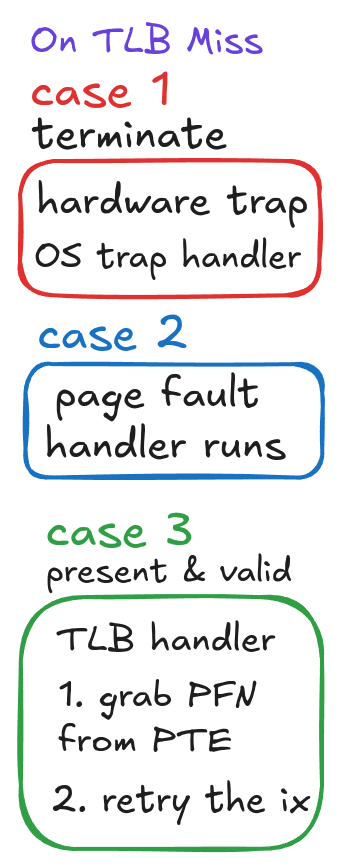
\includegraphics[width=\linewidth]{imgs/swap_cases}
\end{minipage}
\section*{Page-Fault Control Flow Algorithm (Software)}
\begin{minipage}{.72\linewidth}
\begin{lstlisting}[language=c]
PFN = FindFreePhysicalPage()
if (PFN == -1)                 // no free page found
    PFN = EvictPage()          // replacement algo
DiskRead(PTE.DiskAddr, PFN)  // sleep (wait for I/O)
PTE.present = True             // update page table:
PTE.PFN = PFN                  // present/translation
RetryInstruction()             // retry instruction
\end{lstlisting}
\end{minipage}
\begin{minipage}{.28\linewidth}
  \flushleft
  \begin{enumerate}
  \item check any free pages avail
  \item if not, ask bg thread to free
  \item when some pages avail, wake up orig thread
  \end{enumerate}
\end{minipage}

\begin{itemize}
\item when OS notices there're fewer than low watermark (LW) pages avail., a background thread responsible for freeing memory runs
\item bg thread evicts pages until there're high watermark (HW) pages avail.
\item bg swap/page daemon: disk efficiency $\uparrow$; work $\downarrow$, better idle time
\item OS groups pages and swaps them out at once $\to$ $\uparrow$ disk efficiency
\end{itemize}

% \columnbreak
% \section*{Swapping Policies (minimize cache miss/page fetch)}
\begin{itemize}
\item Average Memory Access Time (AMAT)=$T_{M}+(P_{\text{Miss}} + T_{D})$
\item $T_{M}$ the cost of accessing memory; $T_{D}$ the cost of accessing disk
\item $P_{\text{Miss}}$ the probability of not finding  data in cache (a miss) [0.0,1.0]
\item $P_{\text{Miss}} = 0.1$, $T_{D}=10$ms, $T_{M}$=100ns $\to$ AMAT = 1.0001ms
\item $P_{\text{Miss}} = 0.001$ ($P_{\text{Hit}} = 0.999$) $\to$ AMAT = 10.1$\mu$s (100 times faster)
\item In general, $P_{\text{Miss}} + P_{\text{Hit}} = 1.0$
\end{itemize}

\section*{Types of cache misses (3 categories)}
\begin{enumerate}
\item compulsory miss (aka cold-start miss): cache is empty (first reference)
\item capacity miss: no enough space $\to$ evict old to make room for new
\item conflict miss: arises due to (hardware) limits on where the item can be placed in cache.  Conflict miss doesn’t occur in the OS page cache, as the cache is
fully associative (a page can be placed anywhere)
\end{enumerate}

\section*{The optimal policy (by Belady), FIFO, Random, LRU, LFU}
\begin{itemize}
\item replace the page that will be accessed \textbf{furthest in the future}
\item Hard to implement (because hard to predict the future)
\item Useful as an ideal policy to compare with (can't do better than optimal)
\end{itemize}
\begin{itemize}
\item FIFO/Random: might evict important pages (to be ref-ed again soon)
\item \textbf{frequency} a page accessed frequently is perhaps important
\item \textbf{recency} a page accessed recently will perhaps be accessed again
\end{itemize}
\section*{Workload examples (100 unique pages)}
\begin{minipage}{0.33\linewidth}
  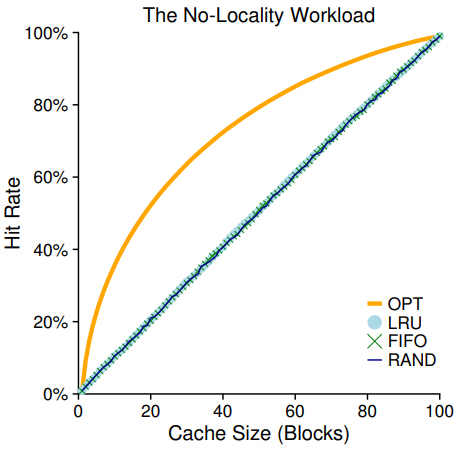
\includegraphics[width=\linewidth,height=3.5cm]{imgs/non_locality_workload}
\end{minipage}
\begin{minipage}{0.34\linewidth}
  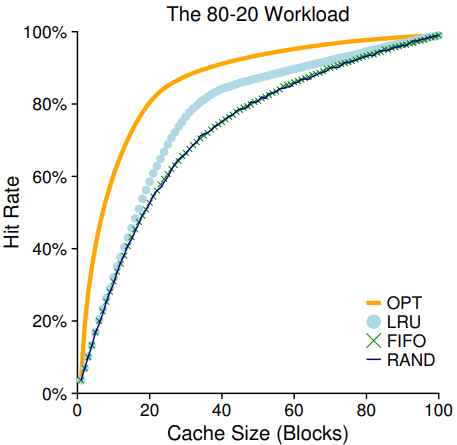
\includegraphics[width=\linewidth,height=3.5cm]{imgs/eight_20_workload}
\end{minipage}
\begin{minipage}{0.33\linewidth}
  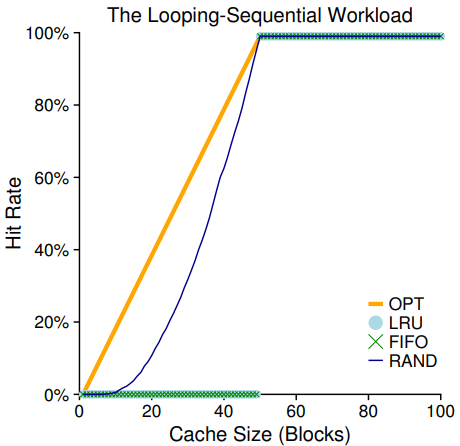
\includegraphics[width=\linewidth,height=3.5cm]{imgs/looping_workload}
\end{minipage}
\begin{minipage}{0.5\linewidth}
  \flushleft
  \begin{enumerate}
  \item no locality $\to$ any policy works
  \item when cache size $>$ workload, swap policy in use doesn't matter
  \item optimal performs better than other realistic policies
  \item for 80-20, LRU does better than random/FIFO
  \end{enumerate}
\end{minipage}
\begin{minipage}{0.5\linewidth}
  \flushleft
  \begin{enumerate}
  \item loops common in applications (eg databases)
  \item worst case scenario for FIFO and LRU
  \item A looping workload with N pages and cache size $<$ N pages always result in
0\% hit rate
  \end{enumerate}
\end{minipage}

\section*{Issues of implementing LRU}
\begin{itemize}
\item implementing history-based policies requires accounting of every memory ref $\to$ performance $\downarrow$ if not careful
\item possible hardware support: update time field in memory for each page
\item OS then scans time fields to find LRU page: expensive if page num $\uparrow$
\end{itemize}
\section*{Approximating LRU: clock algorithm}
\begin{itemize}
\item use a \textbf{use bit} (aka \textbf{reference bit} to page)
\item when page is accessed, set bit to 1 (done by hardware)
\item arrange all pages in a circular list and when replacement occurs
\item if use bit is 1, set it to 0 and move on; if use bit is 0, evict the page
\end{itemize}
\section*{Dirty Pages (regarding clock algorithm: whether a page is modified)}
\begin{itemize}
\item If page has been modified, do not evict (write to disk is expensive)
\item If page is clean, eviction is free (no need to write to disk)
\item hardware support should include a \textbf{dirty bit}
\end{itemize}
\section*{Belady's anomaly}
\begin{itemize}
\item In general, cache size $\uparrow \to$ cache hit rate $\uparrow$ but not true for FIFO
\item stack property: For algorithms (eg LRU) with this property, cache of size N + 1 naturally includes contents of a cache of size N
\item FIFO/Random (among others) do not obey the stack property; susceptible to anomalous behavior
\end{itemize}

% \section*{(most) Locks}
\begin{minipage}{.5\linewidth}
\begin{lstlisting}[language=c,xrightmargin=2pt]
// globally-allocated lock 'mutex'
lock_t mutex; // declare lock var
// ... other work ...
lock(&mutex);
balance = balance + 1;
unlock(&mutex);
\end{lstlisting}
\end{minipage}
\begin{minipage}{.5\linewidth}
  \begin{itemize}
  \item must declare a lock before using it
  \item lock available = unlocked, free $\to$ no thread holds it
  \item lock acquired = locked, held $\to$ exactly one thread holds it (likely in a critical section)
  \end{itemize}
\end{minipage}
\begin{itemize}
\item other info like which thread holds lock or a queue for ordering lock acquisition can be stored in lock but often hidden from user
\item calling \texttt{lock()} will try to acquire lock (1. free; 2. not free)
  \begin{enumerate}
  \item thread acquires lock and enters critical section; \textbf{owner} of lock
  \item thread waits (not return) and cannot enter critical section
  \end{enumerate}
\item calling \texttt{unlock()} will free the lock (1. no waiting thread; 2. opposite)
  \begin{enumerate}
  \item lock becomes free and any thread can try to acquire it
  \item one of waiting threads will acquire lock and enters critical section
  \end{enumerate}

\item \textbf{coarse-grained}: one big lock for access to critical section at any time
\item \textbf{fine-grained}: different locks to protect different data and data structs (allowing more threads in different locked code at once)
\end{itemize}
\section*{Evaluating Locks}
\begin{enumerate}
\item \textbf{correctness} lock provides \textbf{mutual exclusion}
\item \textbf{fairness} each thread gets a fair shot at acquiring the lock (once it's free); no thread contending for the lock starve while doing so
\item \textbf{performance} time overhead added by using the lock:
  \begin{enumerate}
  \item single thread (no contention) $\to$ what is the overhead?
  \item multiple threads contending for lock on single CPU
  \item lock perf. on multiple CPUs and threads contending for the lock
  \end{enumerate}
\end{enumerate}
\begin{minipage}{.5\linewidth}
\begin{lstlisting}[language=c,xrightmargin=2pt]
void lock() { // before entering
  DisableInterrupts();
}
void unlock() { // after leaving
  EnableInterrupts();
}
\end{lstlisting}
\end{minipage}
\begin{minipage}{.5\linewidth}
  \begin{itemize}
  \item one of earliest solution offers mutex by disabling interrupts
  \item code inside critical section (not interrupted) runs as if it were atomic
  \item invented for single-processor systems;  main advantage: simplicity
  \end{itemize}
\end{minipage}
\begin{enumerate}
\item \textbf{insecure} arbitrary thread will need to perform \emph{privileged} ops so greedy/malicious progs can monopolize CPU and exploit system
\item \textbf{importable} not working on multiprocessors: threads enter same critical section via other CPUs $\to$ null effect of disabling interrupts
\item \textbf{buggy} turning off interrupts for too long $\to$ lost useful/critical interrupts that make OS work as expected (e.g. disturb I/O awakening)
\end{enumerate}
Thus, limited use case: OS occasionally uses interrupt masking to guarantee atomicity when accessing its own data structures
\section*{Failed Attempt: Just Using Loads/Stores}
\begin{minipage}{.5\linewidth}
\begin{lstlisting}[language=c,xrightmargin=2pt]
typedef struct __lock_t
{ int flag; } lock_t;

void init(lock_t *mutex) {
  // 0: lock is avail | 1: held
  mutex->flag = 0; }

void lock(lock_t *mutex) {
  while (mutex->flag == 1) // TEST
     ; // spin-wait (do nothing)
  mutex->flag = 1; // now SET it }

void unlock(lock_t *mutex) {
   mutex->flag = 0; }
\end{lstlisting}
\end{minipage}
\begin{minipage}{.5\linewidth}
  \begin{itemize}
  \item use 1 var \texttt{flag} to indicate thread's ownership of lock
  \item when lock not free, other threads \textbf{spin-wait} in while loop
  \item once lock free, waiting thread gets lock $\to$ set flat to 1
  \item correctness problem: both of two threads can set flag to 1 (with interrupts) and enter same critical section $\to$ mutex \textbf{not} guaranteed
  \item performance issue: thread endless checks flag (spin-waiting) and wastes CPU cycles
  \end{itemize}
\end{minipage}
\section*{Working Spin Locks with Test-And-Set (atomic exchange)}
\begin{itemize}
\item test old value and simultaneously setting the mem location to new value
\item return the old value pointed by \texttt{old\_ptr} and set \texttt{new} at same time
\item this sequence of operations is performed \textbf{atomically}
\end{itemize}
\begin{minipage}{.7\linewidth}
\begin{lstlisting}[language=c]
int TestAndSet(int *old_ptr, int new) {
  int old = *old_ptr;// fetch old value at old_ptr
  *old_ptr = new;      // store new into old_ptr
  return old;          // return the old value
}

typedef struct __lock_t { int flag; } lock_t;

// 0: lock is avail, 1: lock is held
void init(lock_t *lock) { lock->flag = 0; }

void lock(lock_t *lock) {
   while (TestAndSet(&lock->flag, 1) == 1)
     ; // spin-wait (do nothing)
}

void unlock(lock_t *lock) { lock->flag = 0; }
\end{lstlisting}
\end{minipage}
\begin{minipage}{.3\linewidth}
  \flushleft
  \begin{itemize}
  \item make both \textbf{test} (old lock value) and \textbf{set} (new value) a single atomic op $\to$ only one thread acquires the lock $\to$ working mutual exclusion primitive
  \item On single CPU, needs a preemptive scheduler (interrupt via timer); otherwise a thread spins on a CPU and never gives it up
  \end{itemize}
\end{minipage}
\begin{enumerate}
\item \textbf{correctness} yes, only a single thread enters critical section at a time
\item \textbf{fairness} not generally, thread may spin forever $\to$ starve/zero fairness
\item \textbf{performance} \textbf{a} on single CPU, pretty bad: if N threads contending for the lock, each thread spins for duration of time slice before being timer-preempted. \textbf{b} on multiple CPU, reasonably well if \# of threads $\approx$ \# of CPUs and critical section is short (wasting fewer CPU cycles)
\end{enumerate}

\section*{Compare-and-Swap (SPARC) or Compare-and-Exchange (x86)}
\begin{minipage}{.65\linewidth}
\begin{lstlisting}[language=c]
// only diff with set-and-test shown below
int CompareAndSwap(int *ptr,
                     int expected, int new)
{
    int original = *ptr;
    if (original == expected)
       *ptr = new;
    return original;
}
void lock(lock_t *lock) {
   while(CompareAndSwap(&lock->flag,0,1) == 1)
      ; // spin
} // more powerful than test-and-set
\end{lstlisting}
\end{minipage}
\begin{minipage}{.35\linewidth}
  \flushleft
  \begin{itemize}
  \item test if value at addr \texttt{ptr} == expected;
  \item if so, update mem location \texttt{ptr} to new.
  \item If not, do nothing.
  \item In either case, return orig val at that mem location, thus allowing the code calling compare-and-swap to know if it succeeded
  \item for lock-free struct
  \end{itemize}
\end{minipage}
a simple spin lock built with it \texttt{==} test-and-set spin lock analyzed above
\section*{Load-Linked + Store-Conditional (MIPS, Alpha, PowerPC, ARM)}
\begin{minipage}{.65\linewidth}
\begin{lstlisting}[language=c]
int LoadLinked(int *ptr) { return *ptr; }
// atomic operation
int StoreConditional(int *ptr, int new) {
  if (no update to *ptr
      since LoadLinked to this address) {
     *ptr = new;
     return 1; // success!
  } else { return 0; }  // failed to update
}
// Using LL/SC To Build A Lock
void lock(lock_t *lock) {
  while (1) {
    while (LoadLinked(&lock->flag) == 1)
       ; // spin until it's zero
    if (StoreConditional(&lock->flag, 1) == 1)
       return;
      // if set-it-to-1 is a success: all done
      // otherwise: try it all over again
    }
}
void unlock(lock_t *lock) { lock->flag = 0; }
\end{lstlisting}
\end{minipage}
\begin{minipage}{.35\linewidth}
  \flushleft
  \begin{itemize}
  \item load-linked operation likes load ix $\to$ fetch a value from addr \texttt{ptr} and place in a register
  \item store-cond succeeds (and updates the val) \emph{only} if no intervening store to the addr has taken place
  \item if succeeded, returns 1; val at \texttt{ptr} $\to$ \texttt{new}
  \item if failed, returns 0; val at \texttt{ptr} \emph{not} updated
  \item suppose 2 threads both exec \texttt{LoadLinked} and proceed to store-cond
  \item at this point only 1 thread will succeed in updating flag to 1
  \end{itemize}
\end{minipage}
\begin{minipage}{.45\linewidth}
\begin{lstlisting}[language=c]
int FetchAndAdd(int *ptr) {
   int old = *ptr;
   *ptr = old + 1;
   return old; }
\end{lstlisting}
\end{minipage}
\begin{minipage}{.55\linewidth}
  \begin{itemize}
  \item atomically increments a val while returning old val at particular addr
  \item In Intel x86, implemented using the ADD instruction with a prefix LOCK
  \end{itemize}
\end{minipage}
\section*{Ticket lock using Fetch-and-Add (ensures progress for all threads)}
\begin{minipage}{.55\linewidth}
\begin{lstlisting}[language=c]
typedef struct __lock_t {
  int ticket;
  int turn;
} lock_t;
void lock_init(lock_t *lock) {
  lock->ticket = 0;
  lock->turn = 0;
}
void lock(lock_t *lock) {
  int myturn;
  myturn = FetchAndAdd(&lock->ticket);
  while (lock->turn != myturn)
     ; // spin
}
void unlock(lock_t *lock) {
   lock->turn = lock->turn + 1;
}
\end{lstlisting}
\end{minipage}
\begin{minipage}{.45\linewidth}
  \flushleft
  \begin{itemize}
  \item when a thread tries to acquire a lock, it first does an \textbf{atomic} fetch-and-add on the ticket
  \item that value is now this thread's ``turn'' (\texttt{myturn})
  \item then use globally shared \texttt{lock->turn} to determine which thread's turn
  \item a thread enters critical section if \texttt{myturn == turn}
  \item unlocking increments the turn so next waiting thread (if any) can enter critical section
  \item thread with ticket will be scheduled later on
  \end{itemize}
\end{minipage}
\section*{Yield (good with 2 threads but worse with more)}
\begin{minipage}{.5\linewidth}
\begin{lstlisting}[language=c]
void init() { flag = 0; }
void lock() {
  while (TestAndSet(&flag, 1) == 1)
    yield(); // give up the CPU
}
void unlock() { flag = 0; }
\end{lstlisting}
\end{minipage}
\begin{minipage}{.5\linewidth}
  \flushleft
  \begin{itemize}
  \item assume OS with \texttt{yeild()} (give up CPU and let others run)
  \item thread may be running, ready, or blocked; \texttt{yeild}: running $\to$ ready
  \item yielding thd \textbf{deschedules} itself
  \item works well with 2 thds (no spin)
  \end{itemize}
\end{minipage}
\begin{itemize}
\item suppose there are 100 threads contending for a lock repeatedly
\item if one thread acquires lock but gets preempted before releasing it, the other 99 will each call \texttt{lock()}, find lock held, and yield CPU
\item if RR sched, each of 99 run-and-yeild before lock-holder runs again
\item no 99 time slice spinning but cost of ctx switch is substantial (waste)
\item this approach does \emph{not} stress starvation: A thread may get
caught in endless yield loop while others repeatedly enter/exit critical section
\end{itemize}
\section*{Lock with queues (correct, reasonably fair, limited spinning)}
\begin{minipage}{.6\linewidth}
\begin{lstlisting}[language=c]
typedef struct __lock_t {
  int flag;
  int guard;
  queue_t *q;
} lock_t;
void lock_init(lock_t *m) {
  m->flag = 0;
  m->guard = 0;
  queue_init(m->q);
}
void lock(lock_t *m) {
  while (TestAndSet(&m->guard, 1) == 1)
     ; //acquire guard lock by spinning
  if (m->flag == 0) {
    m->flag = 1; // lock is acquired
    m->guard = 0;
  } else {
    queue_add(m->q, gettid());
+   setpark();  // avoid wakeup/waiting race
    m->guard = 0;
    park(); // syscall
  }
} // + indicates new code
void unlock(lock_t *m) {
  while (TestAndSet(&m->guard, 1) == 1)
     ; //acquire guard lock by spinning
  if (queue_empty(m->q))// no one wants it
    m->flag = 0;          // let go of lock
  else // hold lock for next thread
    unpark(queue_remove(m->q));
  m->guard = 0;
}
\end{lstlisting}
\end{minipage}
\begin{minipage}{.4\linewidth}
  \flushleft
  \begin{itemize}
  \item this approach doesn't avoid spin-waiting entirely: a spin-lock around \texttt{flag} and \texttt{queue} (lock is using)
  \item \texttt{guard} ensures queue is modified atomically
  \item waiting thread $\to$ queue and \texttt{park()} to sleep
  \item thread releasing lock $\to$ \texttt{unpark()} waiting threads
  \item time spent spinning is quite limited (just a few instructions inside lock and unlock code, instead of user-def critical section)
  \item if thread not acquired lock, adds itself to queue
  \item When a thread woken up, it is as if returning from \texttt{park()}; yet it does not hold \texttt{guard} at that point and thus cannot try to set \texttt{flag} to 1. lock passed directly from releasing-thd to next waiting thd. \texttt{flag} is not set to 0 in-between
  \item \texttt{setpark} makes \texttt{park} return immediately
  \end{itemize}
\end{minipage}

% \section*{Concurrent Counters (initial vs scalable/approximate)}
\begin{minipage}{.5\linewidth}
\begin{lstlisting}[language=c,xrightmargin=4pt]
typedef struct __counter_t {
  int value;
  pthread_mutex_t lock;
} counter_t;
void init(counter_t *c) {
  c->value = 0;
  Pthread_mutex_init(
          &c->lock, NULL);
}
int get(counter_t *c) {
  Pthread_mutex_lock(&c->lock);
  int rc = c->value;
  Pthread_mutex_unlock(&c->lock);
  return rc;
}
\end{lstlisting}
\end{minipage}
\begin{minipage}{.5\linewidth}
\begin{lstlisting}[language=c,xleftmargin=4pt,framextopmargin=2pt]
void increment(counter_t *c) {
  Pthread_mutex_lock(&c->lock);
  c->value++;
  Pthread_mutex_unlock(&c->lock);
}
void decrement(counter_t *c) {
  Pthread_mutex_lock(&c->lock);
  c->value--;
  Pthread_mutex_unlock(&c->lock);
}
\end{lstlisting}
  \begin{itemize}
  \item add locks to every read/write access to shared value
  \item thread-safe but too slow: scales poorly as \#threads grows
  \end{itemize}
\end{minipage}
\begin{lstlisting}[language=c]
typedef struct __counter_t {
    int global;                         // global count
    pthread_mutex_t glock;              // global lock
    int local[NUMCPUS];                 // per-CPU count
    pthread_mutex_t llock[NUMCPUS]; // ... and locks
    int threshold;                      // update freq
} counter_t;
// record threshold, init locks and vals of all local cnt/gloabl cnt
void init(counter_t *c, int threshold) {
    c->threshold = threshold;
    c->global = 0;
    pthread_mutex_init(&c->glock, NULL);
    int i;
    for (i = 0; i < NUMCPUS; i++) {
       c->local[i] = 0;
       pthread_mutex_init(&c->llock[i], NULL);
  }
}

// usually, just grab local lock and update local amount;
// once above `threshold', grab global lock, transfer local vals to it
void update(counter_t *c, int threadID, int amt) {
    int cpu = threadID % NUMCPUS;
    pthread_mutex_lock(&c->llock[cpu]);
    c->local[cpu] += amt;
    if (c->local[cpu] >= c->threshold) {
        // transfer to global (assumes amt > 0)
        pthread_mutex_lock(&c->glock);
        c->global += c->local[cpu];
        pthread_mutex_unlock(&c->glock);
        c->local[cpu] = 0;
    }
    pthread_mutex_unlock(&c->llock[cpu]);
}
\end{lstlisting}
\begin{minipage}{.48\linewidth}
\begin{lstlisting}[language=c]
int get(counter_t *c) {
  pthread_mutex_lock(&c->glock);
  int val = c->global;
  pthread_mutex_unlock(&c->glock);
  return val; // only approximate!
}
\end{lstlisting}
\end{minipage}
\begin{minipage}{.52\linewidth}
  \centering
  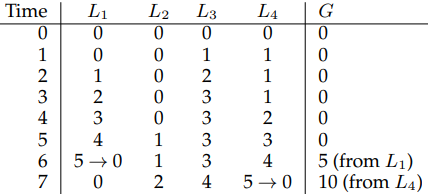
\includegraphics[width=.85\linewidth]{imgs/tracing_approx_cnter}
\end{minipage}
\begin{minipage}{.5\linewidth}
  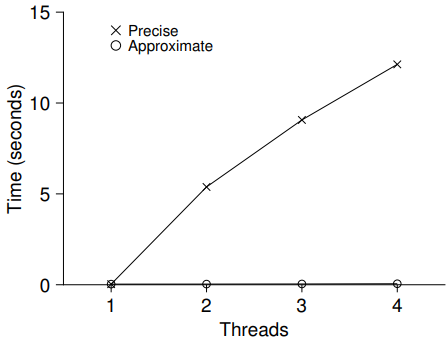
\includegraphics[width=.8\linewidth]{imgs/precise_approx_cnter}
\end{minipage}
\begin{minipage}{.5\linewidth}
  \centering
  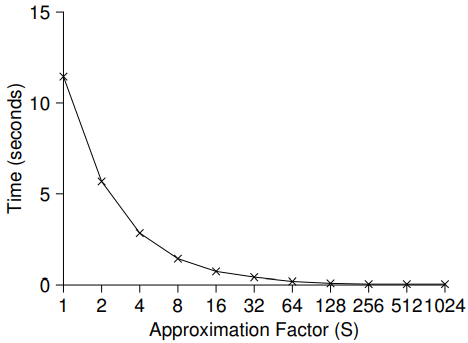
\includegraphics[width=.8\linewidth]{imgs/scaling_approx_cnter}
\end{minipage}
\section*{Concurrent Linked List (insertion and lookup)}
\begin{minipage}{.52\linewidth}
\begin{lstlisting}[language=c,xleftmargin=-4pt]
// basic node structure
typedef struct __node_t {
   int               key;
   struct __node_t   *next;
} node_t;
// basic list struct, used per list
typedef struct __list_t {
    node_t           *head;
    pthread_mutex_t  lock;
} list_t;
void List_Init(list_t *L) {
  L->head = NULL;
  pthread_mutex_init(&L->lock, NULL);
}
\end{lstlisting}
\end{minipage}
\begin{minipage}{.48\linewidth}
  \flushleft
  \begin{itemize}
  \item acquire lock upon entry to insert fn and release it upon exit
  \item if \texttt{malloc()} fails, the code must also release lock
  \item nearly 40\% bugs found on such rarely-taken code path
  \item \textbf{rearrange} code so that lock and release only surround actual critical section in insert code, $\because$ part of insert need no locking
  \item assume \texttt{malloc} itself thread-safe $\to$ no race conds and only updating shared list needs lock
  \end{itemize}
\end{minipage}
\begin{minipage}{.53\linewidth}
\begin{lstlisting}[language=c,xleftmargin=-4pt]
int List_Insert(list_t *L,int key)
{
  pthread_mutex_lock(&L->lock);
  node_t *new = malloc(sizeof node_t);
  if (new == NULL) {
    perror("malloc");
    pthread_mutex_unlock(&L->lock);
    return -1; // fail
  }
  new->key = key;
  new->next = L->head;
  L->head = new;
  pthread_mutex_unlock(&L->lock);
  return 0; // success
}
\end{lstlisting}
\end{minipage}
\begin{minipage}{.53\linewidth}
\begin{lstlisting}[language=c,xleftmargin=2pt]
int List_Insert(list_t *L, int key)
{
 node_t *new = malloc(sizeof node_t);
 if (new == NULL) {
    perror("malloc");
    return -1;
 }
 new->key = key;
 // just lock critical section
 pthread_mutex_lock(&L->lock);
 new->next = L->head;
 L->head = new;
 pthread_mutex_unlock(&L->lock);
 return 0; // success
}
\end{lstlisting}
\end{minipage}
\begin{minipage}{.53\linewidth}
\begin{lstlisting}[language=c,xleftmargin=-4pt]
int List_Lookup(list_t *L, int key)
{
  pthread_mutex_lock(&L->lock);
  node_t *curr = L->head;
  while (curr) {
    if (curr->key == key) {
      pthread_mutex_unlock(&L->lock);
      return 0; // success
    }
    curr = curr->next;
 }
 pthread_mutex_unlock(&L->lock);
 return -1; // failure
}
\end{lstlisting}
\end{minipage}
\begin{minipage}{.53\linewidth}
\begin{lstlisting}[language=c,xleftmargin=2pt]
int List_Lookup(list_t *L, int key) {
  int rv = -1;
  pthread_mutex_lock(&L->lock);
  node_t *curr = L->head;
  while (curr) {
    if (curr->key == key) {
      rv = 0;
      break;
    }
    curr = curr->next;
  }
  pthread_mutex_unlock(&L->lock);
  return rv; // common exit path
}
\end{lstlisting}
\end{minipage}
\begin{itemize}
\item improved impl does \emph{not} scale well; single lock for entire list: bottleneck
\item \textbf{hand-over-hand locking} (lock coupling) enables more concurrency:
\item One lock per node – instead of a single lock for the entire list
\item While traversing, grab next nd's lock, then release current nd's lock
\item in practice, hard to get faster than simple single lock approach, as overheads of acquiring/releasing locks for each node of list is prohibitive
\item Even with very large lists and a large \# threads, concurrency of multiple ongoing traversals is unlikely faster than simply grabbing a single lock, performing an operation, and releasing it
\item general theme: using one global lock for the entire data structures always ensure thread safety, but at cost of concurrency (performance)
\item to improve performance: increase granularity of critical regions and assign different locks to these regions
\end{itemize}
\section*{Concurrent Queue (by Michael and Scott)}
\begin{itemize}
\item use two locks: one for head of queue and one for its tail
\item in common case, enqueue routine will only access tail lock, and dequeue only head lock (goal: allow concurrent enqueue and dequeue ops)
\item add a dummy node in init $\to$ enable separation of head and tail ops
\end{itemize}
\begin{lstlisting}[language=c,xleftmargin=16pt,xrightmargin=6pt,framextopmargin=3pt]
typedef struct __node_t {
    int             value;
    struct __node_t *next;
} node_t;

typedef struct __queue_t {
    node_t          *head;
    node_t          *tail;
    pthread_mutex_t head_lock, tail_lock;
} queue_t;

void Queue_Init(queue_t *q) {
    // allocate a dummy node
    node_t *tmp = malloc(sizeof(node_t));
    tmp->next = NULL;
    q->head = q->tail = tmp;
    pthread_mutex_init(&q->head_lock, NULL);
    pthread_mutex_init(&q->tail_lock, NULL);
}

void Queue_Enqueue(queue_t *q, int value) {
    node_t *tmp = malloc(sizeof(node_t));
    assert(tmp != NULL);
    tmp->value = value;
    tmp->next = NULL;

    pthread_mutex_lock(&q->tail_lock);
    q->tail->next = tmp;
    q->tail = tmp;
    pthread_mutex_unlock(&q->tail_lock);
}

int Queue_Dequeue(queue_t *q, int *value) {
    pthread_mutex_lock(&q->head_lock);
    node_t *tmp = q->head;
    node_t *new_head = tmp->next;
    if (new_head == NULL) {
       pthread_mutex_unlock(&q->head_lock);
       return -1; // queue was empty
    }
    *value = new_head->value;
    q->head = new_head;
    pthread_mutex_unlock(&q->head_lock);
    free(tmp);
    return 0;
}
\end{lstlisting}
\begin{lstlisting}[language=c,xleftmargin=16pt,xrightmargin=6pt]
#define BUCKETS (101) // built with left concurrent linked list
typedef struct __hash_t {
    list_t lists[BUCKETS];
} hash_t;
void Hash_Init(hash_t *H) {
    int i;
    for (i = 0; i < BUCKETS; i++) // use a lock per hash bucket
       List_Init(&H->lists[i]);
}
int Hash_Insert(hash_t *H, int key) {
    return List_Insert(&H->lists[key % BUCKETS], key);
}
int Hash_Lookup(hash_t *H, int key) {
    return List_Lookup(&H->lists[key % BUCKETS], key);
}
\end{lstlisting}
\begin{itemize}
\item correctness first: for concur data structs, one big lock generally works
\item general guide for performance: break critical regions into separate smaller ones and apply separate locks to them
\item need to consider overhead of lock (and context switching) $\to$ more threads may not mean faster execution
\end{itemize}

% \section*{Condition Variable (check a cond before continuing exec)}
\begin{minipage}{.58\linewidth}
\begin{lstlisting}[language=c]
volatile int done = 0;
void *child(void *arg) {
  printf("child\n");
  done = 1;
  return NULL;
}
int main(int argc, char *argv[]) {
  printf("parent: begin\n");
  pthread_t c;
  // create a child
  Pthread_create(&c, NULL, child, NULL);
  while (done == 0)
     ; // spin
  printf("parent: end\n");
  return 0;
}
\end{lstlisting}
\end{minipage}
\begin{minipage}{.42\linewidth}
  \flushleft
  \begin{itemize}
  \item expected output:
    \begin{itemize}
    \item[] \texttt{parent}: \texttt{begin}
    \item[] \texttt{child}
    \item[] \texttt{parent}: \texttt{end}
    \end{itemize}
  \item easy solution: spin on a cond var until it changes
  \item it works but \mo{very} \mo{inefficient}
  \item spinning wastes CPU cycles
  \item desired: put parent to sleep while waiting for child doing its work and then wake parent up to proceed
  \item need a condition variable as a more efficient checkpoint
  \end{itemize}
\end{minipage}
\begin{lstlisting}[language=c]
// referred to as wait() and signal() for simplicity hereafter
pthread_cond_wait(pthread_cond_t *c, pthread_mutex_t *m);
pthread_cond_signal(pthread_cond_t *c); // ^ take mutex as arg
\end{lstlisting}
\begin{lstlisting}[language=c]
int done = 0;
pthread_mutex_t m = PTHREAD_MUTEX_INITIALIZER;
pthread_cond_t c = PTHREAD_COND_INITIALIZER;
\end{lstlisting}
\begin{minipage}{.56\linewidth}
\begin{lstlisting}[language=c]
void thr_exit() {
  Pthread_mutex_lock(&m);
  done = 1;
  Pthread_cond_signal(&c);
  Pthread_mutex_unlock(&m);
}
void *child(void *arg) {
  printf("child\n");
  thr_exit();
  return NULL;
}
void thr_join() {
  Pthread_mutex_lock(&m);
  while (done == 0) // better than if
     Pthread_cond_wait(&c, &m);
  Pthread_mutex_unlock(&m);
}
int main(int argc, char *argv[]) {
  printf("parent: begin\n");
  pthread_t p;
  Pthread_create(&p, NULL, child, NULL);
  thr_join();
  printf("parent: end\n");
  return 0;
}
\end{lstlisting}
\end{minipage}
\begin{minipage}{.44\linewidth}
  \flushleft
  \begin{itemize}
  \item \texttt{wait()} puts calling thread to sleep and release the lock (done \mr{atomically})
  \item when sleeping thread wakes up (after some other thread signal), it must \mb{reacquire} lock before returning to caller
  \item thus preventing certain race conds when a thread is trying to put itself to sleep (while others contending for lock)
  \item suppose 1 CPU and 2 threads
  \end{itemize}
  \begin{enumerate}
  \item parent creates child and immediately calls \texttt{join()} to wait for child
  \item parent acquires lock, sees child not done $\to$ \texttt{wait()} (also release the lock)
  \item child grabs lock, runs, prints, then \texttt{exit()} to signal parent
  \item parent returns from \texttt{wait()}, reholds lock, unlocks, done
  \end{enumerate}
\end{minipage}
\begin{enumerate}
\item child runs immediately upon creation, sets \texttt{done} to 1, \texttt{signal()} to wake sleeping thread, but there is none, so child done and returns
\item parent runs \texttt{join()}, sees \texttt{done} is 1, so does \mr{not} wait and just returns
\end{enumerate}
\begin{minipage}{.5\linewidth}
\begin{lstlisting}[language=c,xrightmargin=2pt]
void thr_exit() {
  Pthread_mutex_lock(&m);
  Pthread_cond_signal(&c);
  Pthread_mutex_unlock(&m); }
void thr_join() {
  Pthread_mutex_lock(&m);
  Pthread_cond_wait(&c, &m);
  Pthread_mutex_unlock(&m); }
\end{lstlisting}
\end{minipage}
\begin{minipage}{.5\linewidth}
  \flushleft
  \begin{itemize}
  \item if no condition variable \texttt{done}
  \item child may run immediately and \texttt{exit()}, then \texttt{signal()} main
  \item but main has \mr{not} fallen asleep
  \item since child already \texttt{signal()} before and won't do that again, when main thread try to \texttt{wait()}, it waits forever $|$ [if no mutex $\downarrow$]
  \end{itemize}
\end{minipage}
\begin{minipage}{.5\linewidth}
\begin{lstlisting}[language=c,xrightmargin=2pt]
void thr_exit() { // signal first
 done = 1; // no one to wake up
 Pthread_cond_signal(&c); }
\end{lstlisting}
\end{minipage}
\begin{minipage}{.5\linewidth}
\begin{lstlisting}[language=c,xleftmargin=2pt]
void thr_join() { // wait later ->
 if (done == 0)    // sleep forever
   Pthread_cond_wait(&c); }
\end{lstlisting}
\end{minipage}
\section*{The Producer/Consumer (Bounded Buffer) Problem}
\begin{itemize}
\item buffer is shared by a single producer and a single consumer
\item consumer \mo{wait}s for item avail. in buffer before reading; producer \mo{wait}s buffer to be empty before writing: need mutex + cond var
\end{itemize}
\begin{minipage}{.5\linewidth}
\begin{lstlisting}[language=c,xleftmargin=0pt,xrightmargin=2pt,frame=lines]
int buffer; // single-item buffer
int count = 0; // init empty
// assume buffer empty
void put(int value) {
  assert(count == 0);
  count = 1;
  buffer = value;
} // broken `put', see below
int get() { // assume buffer full
  assert(count == 1);
  count = 0;
  return buffer;
} // broken `get', see below
\end{lstlisting}
\end{minipage}
\begin{minipage}{.5\linewidth}
\begin{lstlisting}[language=c,xleftmargin=2pt,xrightmargin=2pt,frame=lines]
int buffer[MAX]; int count = 0;
int fill_ptr = 0; int use_ptr = 0;
void put(int value) {
  buffer[fill_ptr] = value;
  fill_ptr = (fill_ptr + 1) % MAX;
  count++;
} // correct `put', see right ->
int get() {
  int tmp = buffer[use_ptr];
  use_ptr = (use_ptr + 1) % MAX;
  count--;
  return tmp;
} // correct `get', see right ->
\end{lstlisting}
\end{minipage}

\begin{minipage}{.63\linewidth}
\begin{lstlisting}[language=c,xleftmargin=0pt]
int loops;      // must init somewhere
cond_t cond;    // broken when two consumers
mutex_t mutex; // see text on the right
void *producer(void *arg) {
  int i;
  for (i = 0; i < loops; i++) {
    thread_mutex_lock(&mutex);              // p1
    if (count == 1)                         // p2
      Pthread_cond_wait(&cond, &mutex); // p3
    put(i);                                 // p4
    Pthread_cond_signal(&cond);             // p5
    Pthread_mutex_unlock(&mutex);           // p6
  }
}
void *consumer(void *arg) {
  int i;
  for (i = 0; i < loops; i++) {
    Pthread_mutex_lock(&mutex);             // c1
    if (count == 0)                         // c2
      Pthread_cond_wait(&cond, &mutex); // c3
    int tmp = get();                        // c4
    Pthread_cond_signal(&cond);             // c5
    Pthread_mutex_unlock(&mutex);           // c6
    printf("%d\n", tmp);
  }
}
\end{lstlisting}
\end{minipage}
\begin{minipage}{.4\linewidth}
  \flushleft
  \begin{itemize}
  \item works well \mo{only} for single producer/consumer
  \item if with $p_1$ and $c_1$, $c_2$:
  \item $c_1$ runs first, acquires lock \mb{c1}, checks buf \mb{c2}, which is empty, so it releases lock and waits \mb{c3} (go to sleep)
  \item $p_1$ runs, acquires lock \mb{p1}, checks \mb{p2} and fills buf \mb{p4}, wakes up $c_1$ \mb{p5} (buf full). $p_1$ goes to sleep \mb{p6}, \mb{p1}-\mb{p3}
  \item $c_2$ runs (before $c_1$ has a chance) and consumes existing item \mb{c1}-\mb{c2}, \mb{c4}-\mb{c6}, skipping \mb{c3} due to buf full
  \item $c_1$ resumes, acquires lock, attempts to \texttt{get()} [\mb{c4}], \mr{without re-checking} \texttt{count}, as check was done before it went to sleep \mb{c2}
  \item Signaling only wakes up thread; it is a \mr{hint} that state
of world has changed
  \end{itemize}
\end{minipage}
\begin{minipage}{.64\linewidth}
\begin{lstlisting}[language=c,xleftmargin=0pt]
void *producer(void *arg) {
  int i;
  for (i = 0; i < loops; i++) {
    thread_mutex_lock(&mutex);              // p1
-   if (count == 1)                         // p2
+   while (count == 1)                      // p2
      Pthread_cond_wait(&cond, &mutex); // p3
    put(i);                                 // p4
void *consumer(void *arg) {
  int i;
  for (i = 0; i < loops; i++) {
    Pthread_mutex_lock(&mutex);             // c1
-   if (count == 1)                         // c2
+   while (count == 0)                      // c2
      Pthread_cond_wait(&cond, &mutex); // c3
    int tmp = get();                        // c4
\end{lstlisting}
\end{minipage}
\begin{minipage}{.4\linewidth}
  \flushleft
  \begin{itemize}
  \item fix: change \texttt{if} to \texttt{while}
  \item when $c_1$ wakes up, it \mo{recheck}s \texttt{cond} \mb{c2}; if buf empty, $c_1$ sleeps (\mb{c3})
  \item there is \mr{still one bug}:
  \item $c_1$, $c_2$ runs first and both go to sleep (\mb{c3})
  \item $p_1$ runs, fills buf, wakes $c_1$, loops back (\mb{p1}-\mb{p6}), waits on same cond (buf full $\to$ go to sleep, \mb{p2}-\mb{p3})
  \item $c_1$ wakes, returns from \texttt{wait()} \mb{c3}, re-checks \mb{c2}, takes val \mb{c4} (continued ...)
  \end{itemize}
\end{minipage}
\vspace{-.8em}
\begin{itemize}
\item if $c_1$ wakes $c_2$ (\mb{c5}), $c_2$ finds buf empty (\mb{c2}) and goes back to sleep (\mb{c3})
\item since no \mb{c5} from $c_2$, $p_1$ keeps sleeping, $c_1$ falls asleep \mb{c1}-\mb{c3}; all sleeping...
\item Signaling must be more directed: consumer should wake only producers
\item producers wait on cond \texttt{empty} and signal \texttt{fill}; consumers wait on \texttt{fill} and signal \texttt{emtpy}
\item a consumer never accidentally wakes a consumer and vice versa
\end{itemize}
\begin{minipage}{.55\linewidth}
\begin{lstlisting}[language=c,xleftmargin=-1em,xrightmargin=-4pt,frame=lines]
cond_t empty, fill; mutex_t mutex;
void *producer(void *arg) {
  int i;
  for (i = 0; i < loops; i++) {
    thread_mutex_lock(&mutex);
    while (count == 1)
     Pthread_cond_wait(&empty,&mutex);
    put(i);
    Pthread_cond_signal(&fill);
    Pthread_mutex_unlock(&mutex);
  }
}
\end{lstlisting}
\end{minipage}
\begin{minipage}{.55\linewidth}
\begin{lstlisting}[language=c,xleftmargin=-2.8em,frame=lines]
void *consumer(void *arg) {
  int i;
  for (i = 0; i < loops; i++) {
    Pthread_mutex_lock(&mutex);
    if (count == 0)
      Pthread_cond_wait(&fill,&mutex);
    int tmp = get();
    Pthread_cond_signal(&empty);
    Pthread_mutex_unlock(&mutex);
    printf("%d\n", tmp);
  }
}
\end{lstlisting}
\end{minipage}
\section*{Covering Conds (covers all cases where a thread needs to wake up)}
\begin{itemize}
\item \texttt{wait()} and \texttt{signal()} approach to thread synchronization assumes the waiting condition is the \textbf{same} for all threads
\item When multiple waiting threads have different conditions: a multi-thread memory allocator $\to$ When a thread frees memory, it should signal which thread to indicate more memory is available?
\end{itemize}
\begin{minipage}{.6\linewidth}
\begin{lstlisting}[language=c,xleftmargin=4pt]
// how many bytes of the heap are free
int bytesLeft = MAX_HEAP_SIZE;
// need lock and condition
cond_t c;  mutex_t m;
void *allocate(int size) {
  Pthread_mutex_lock(&m);
  while (bytesLeft < size)
    Pthread_cond_wait(&c, &m);
  void *ptr = ...; // get mem from heap
  bytesLeft -= size;
  Pthread_mutex_unlock(&m);
  return ptr;
}
void free(void *ptr, int size) {
  Pthread_mutex_lock(&m);
  bytesLeft += size;
- Pthread_cond_signal(&c);// signal whom?
+ Pthread_cond_broadcast(&c);
  Pthread_mutex_unlock(&m);
 }
\end{lstlisting}
\end{minipage}
\begin{minipage}{.4\linewidth}
  \flushleft
  \begin{itemize}
  \item assume 0 bytes free now
  \item $T_a$ calls \texttt{allocate(100)}
  \item $T_b$ calls \texttt{allocate(10)}
  \item Both $T_a$ and $T_b$ wait on cond and go to sleep due to no enough free bytes to satisfy either of requests
  \item $T_c$ calls \texttt{free(50)} and try to signal a thread
  \item it might wake $T_a$ instead of $T_b$ (suitable in this case)
  \item $T_a$ remains waiting and code not working
  \item Lampson and Redell suggest to wake up \mb{all} waiting threads by \texttt{phthread\_cond\_broadcast()}
  \end{itemize}
\end{minipage}
The downside is a negative performance impact: needlessly wake up many waiting threads that shouldn't (yet) be awake. Those threads will simply wake up, re-check cond, and then go immediately back to sleep
\begin{tcolorbox}[left=0mm, top=1mm, right=0mm, rightlower=0mm, bottom=1mm,
  title=Always hold the lock while signaling,halign title=center]
There are some cases where it is likely OK not to, but probably is something you should avoid. Thus, for simplicity, \textbf{hold the lock when calling signal}. The converse of this tip -- hold lock when calling wait -- is \textbf{mandated} by the semantics of wait: wait always
(a) assumes lock is held when calling it, (b) releases said lock when
putting caller to sleep, and (c) re-acquires lock just before returning. Thus, the generalization is correct:\textbf{ hold the lock when calling signal or wait}, and you will always be in good shape.
\end{tcolorbox}
\begin{tcolorbox}[left=0mm, top=1mm, right=0mm, rightlower=0mm, bottom=1mm,
  title=Use \texttt{while} (not \texttt{if}) for conditions,
  halign title=center]
When checking for a condition in a multi-threaded program, using a
\texttt{while} loop is always correct; using an if statement only might be, depending on what signaling does. Using while loops around conditional checks also handles the case where \textbf{spurious wakeups} occur. In some thread packages, due to implementation details, it's possible that 2 threads get woken up though a single signal. Spurious wakeups are further reason to re-check the condition a thread is waiting on.
\end{tcolorbox}

% \section*{Semaphores (yet another synchronization primitive)}
\begin{itemize}
\item semaphore is just an integer value, accompanied by a queue of threads (waiting for signals) and manipulated with 2 routines: \texttt{P()} and \texttt{V()}
\item in POSIX, \texttt{P()} $\to$ \texttt{sem\_wait()}; \texttt{V()} $\to$ \texttt{sem\_post()}; \mo{must first} \texttt{sem\_init()}
\item tweaking init sem vals to impl. locks, cond vars, other conc primitives
\end{itemize}
\begin{lstlisting}[language=c]
#include <semaphore.h> // if pshared == 0: sem shared btw thds in same
int sem_init(sem_t *sem, int pshared, unsigned int value); // process
int sem_wait(sem_t *sem); // wait on a semaphore
int sem_post(sem_t *sem); // signal the waiting threads
\end{lstlisting}
\begin{minipage}{0.6\linewidth}
\begin{lstlisting}[language=c]
int sem_wait(sem_t *s) {
  /* decrement semaphore `s' by one
  wait if semaphore `s' is negative */
} // assume both wait/post exec atomically
int sem_post(sem_t *s) {
  /* increment semaphore `s' by one
  if waiting threads >= 1, wake one */
}
\end{lstlisting}
\end{minipage}
\begin{minipage}{0.4\linewidth}
\begin{lstlisting}[language=c,xleftmargin=2pt,xrightmargin=2pt]
sem_t m;
// init to X;
// X should be 1 at first
sem_init(&m, 0, X);
/* used as a lock */
sem_wait(&m);
// critical section here
sem_post(&m);
\end{lstlisting}
\end{minipage}
\section*{Binary Semaphores (Locks, code at above right)}
For $N > 1$ threads, the 1st thread to execute \texttt{sem\_wait()}
immediately brings \texttt{s} to 0; other threads will be forced to wait\\
\begin{minipage}{.48\linewidth}
\begin{tabular}[th]{lll}
  \hline
  \multicolumn{3}{l}{trace single T using a sem}\\
  \textbf{sem} & $T_0$ & $T_1$\\
  \hline
  1 & & \\
  1 & call \texttt{sem\_wait()} & \\
  0 & \texttt{sem\_wait()} returns & \\
  0 & (\texttt{crit sect}) & \\
  0 & call \texttt{sem\_post()} & \\
  1 & \texttt{sem\_post()} returns\\
  \hline
\end{tabular}
\end{minipage}
\begin{minipage}{.52\linewidth}
  \flushleft
  \begin{itemize}
  \item $T_0$ calls \texttt{sem\_wait()}, dec \texttt{sem}: $1 \to 0$
  \item then $T_0$ will wait only if sem $\leq$ 0
  \item $\because$ \texttt{sem == 0} now, \texttt{sem\_wait()} will simply return and $T_0$ will continue
  \item $T_0$ now free to enter critical sect.
  \item If no other thd tries to acquire lock while $T_0$ in critical sect, when $T_0$ calls \texttt{sem\_post()}, it will restore \texttt{sem} ($0 \to 1$) and wake no waiting thread, $\because$ there are none
  \end{itemize}
\end{minipage}
Run (running); Ready (runnable not running); Sleep (thread is blocked)
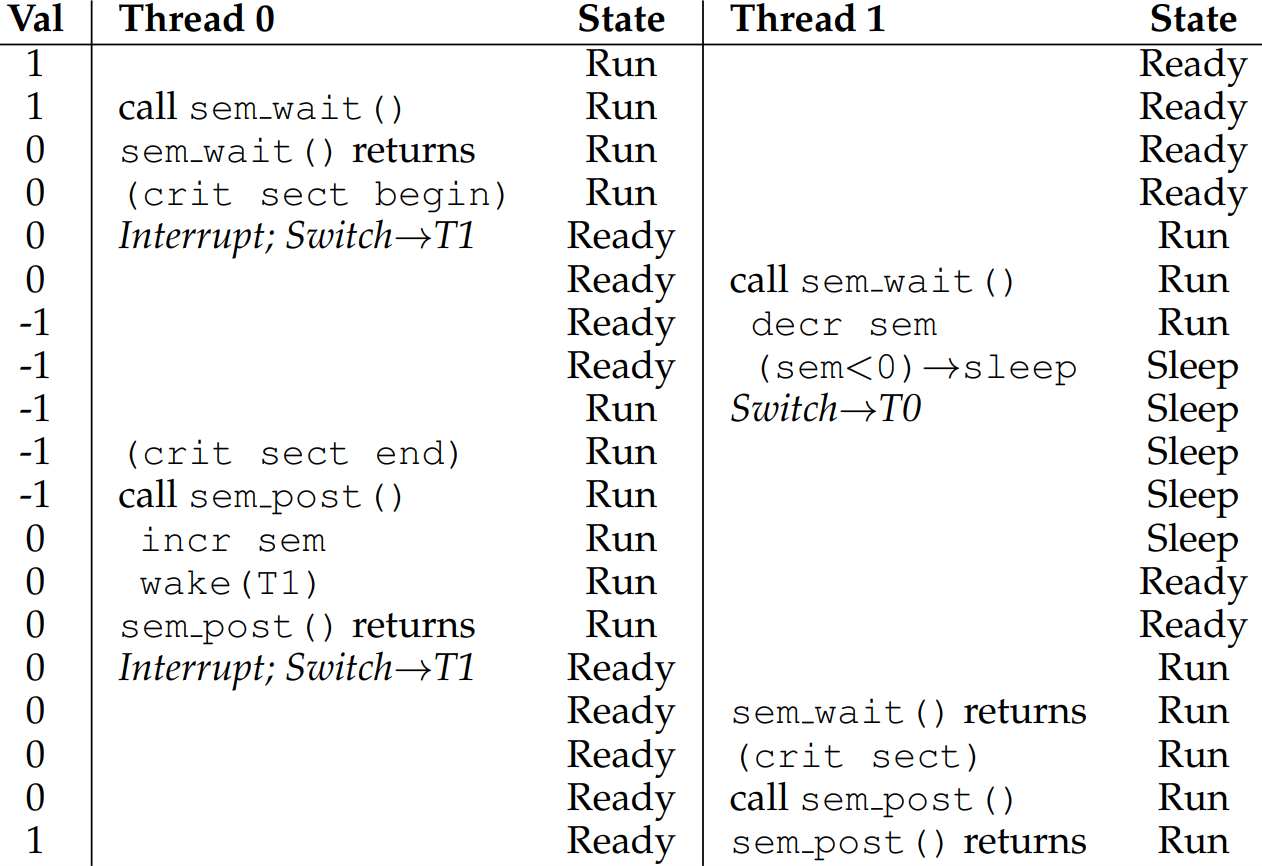
\includegraphics[width=\linewidth,height=6cm]{imgs/twots_usesem2}
\section*{Semaphores for ordering events in concurrent programs}
\begin{minipage}{.4\linewidth}
\begin{lstlisting}[language=c,xleftmargin=2pt,xrightmargin=2pt]
sem_t s; // expected:
/* parent: begin
   child
   parent: end */
void *child(void *arg) {
  printf("child\n");
  sem_post(&s); // signal
  return NULL;
}
\end{lstlisting}
\end{minipage}
\begin{minipage}{.6\linewidth}
\begin{lstlisting}[language=c,xleftmargin=2pt,xrightmargin=2pt]
int main(int argc, char *argv[]) {
  sem_init(&s, 0, X); // X should be 0
  printf("parent: begin\n");
  pthread_t c;
  pthread_create(&c, NULL, child, NULL);
  sem_wait(&s); // wait here for child
  printf("parent: end\n");
  return 0;
} // simulate pthread_join()
\end{lstlisting}
\end{minipage}
% needed this empty line

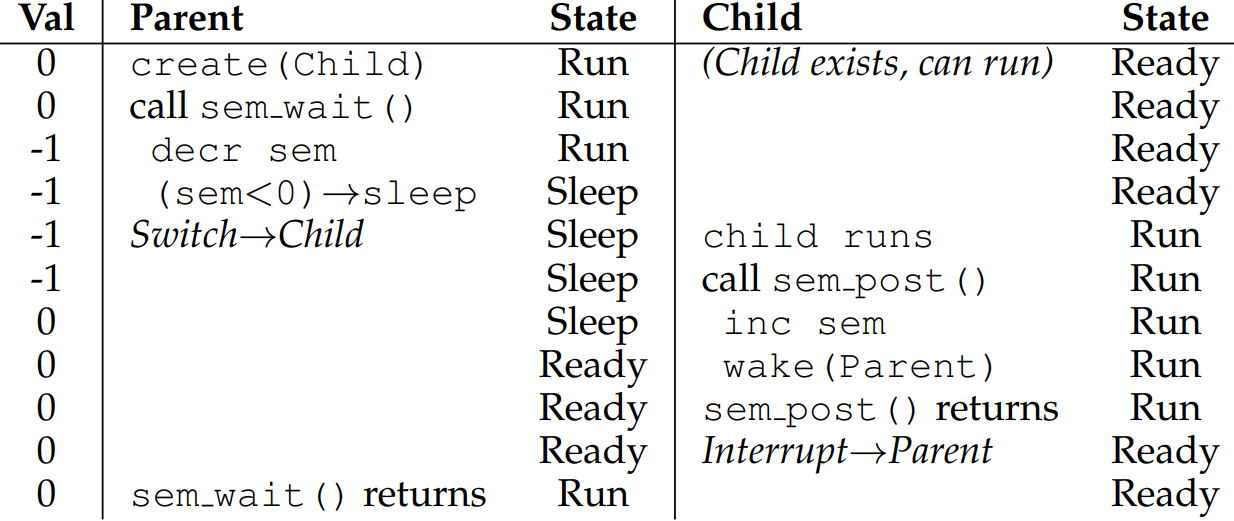
\includegraphics[width=\linewidth,height=4cm]{imgs/pwaitschd}
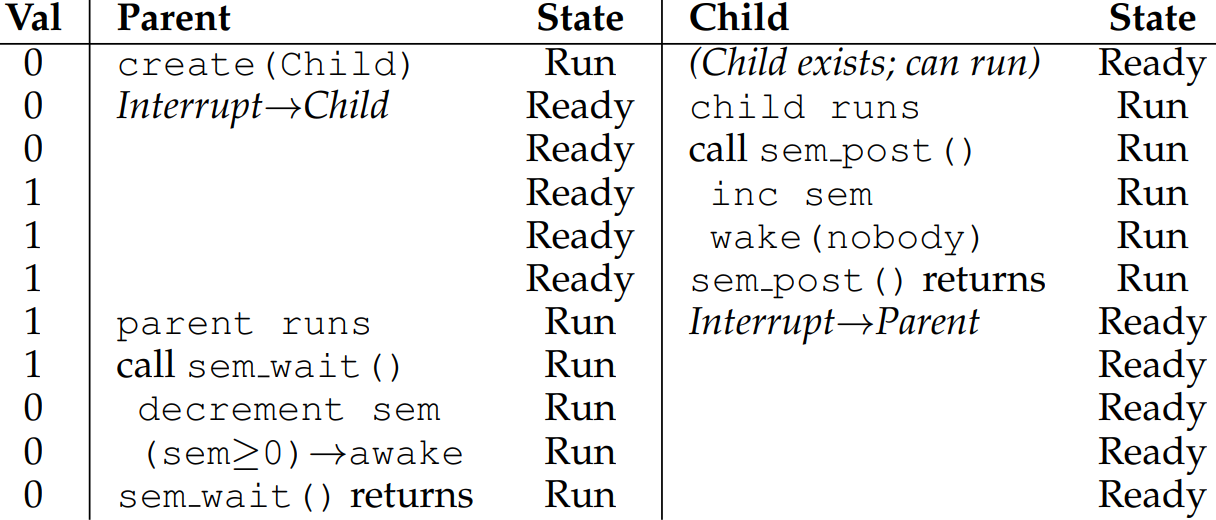
\includegraphics[width=\linewidth,height=4cm]{imgs/chdwaitsp}
\begin{minipage}{.5\linewidth}
\begin{lstlisting}[language=c,xleftmargin=2pt,xrightmargin=2pt]
int buffer[MAX]; // assume MAX = 1
int fill = 0;
int use = 0;
int main(int argc, char *argv[]) {
  // ... init empty = MAX
  sem_init(&empty, 0, MAX);
  sem_init(&full, 0, 0);
  // ... init full = 0
} // assume running on 1 CPU
\end{lstlisting}
\end{minipage}
\begin{minipage}{.5\linewidth}
\begin{lstlisting}[language=c,xleftmargin=2pt,xrightmargin=2pt]
void put(int value) {
  buffer[fill] = value;       // L F1
  fill = (fill + 1) % MAX; // L F2
} // put/get works only if MAX = 1
int get() {
  int tmp = buffer[use]; // L G1
  use = (use + 1) % MAX; // L G2
  return tmp;
}
\end{lstlisting}
\end{minipage}
\begin{minipage}{.5\linewidth}
\begin{lstlisting}[language=c,xleftmargin=2pt,xrightmargin=2pt]
sem_t empty; sem_t full;
void *producer(void *arg) {
  int i;
  for (i = 0; i < loops; i++) {
    sem_wait(&empty); // Line P1
    put(i);             // Line P2
    sem_post(&full);    // Line P3
  }// 2. producer runs & puts P1-2
}  // 3. signals P3 or waits P3-P1
\end{lstlisting}
\end{minipage}
\begin{minipage}{.5\linewidth}
\begin{lstlisting}[language=c,xleftmargin=2pt,xrightmargin=2pt]
void *consumer(void *arg) {
  int tmp = 0;
  while (tmp != -1) {
    sem_wait(&full);    // Line C1
    tmp = get();        // Line C2
    sem_post(&empty);  // Line C3
    printf("%d\n", tmp);
  }// 1. consumer runs & waits C1
}  // 4. wake/take C1-C3 & post C3
\end{lstlisting}
\end{minipage}
\begin{minipage}{.5\linewidth}
\begin{lstlisting}[language=c,xleftmargin=2pt,xrightmargin=2pt,framexbottommargin=2pt]
void *producer(void *arg) {
  int i;
  for (i = 0; i < loops; i++) {
+   sem_wait(&mutex); // Line P0
    sem_wait(&empty); // Line P1
    put(i);             // Line P2
    sem_post(&full);  // Line P3
+   sem_post(&mutex); // Line P4
  }// 3. producer now runs P0
}  // 4. lock held -> deadlock
void *consumer(void *arg) {
  int i;
  for (i = 0; i < loops; i++) {
+   sem_wait(&mutex); // Line C0
    sem_wait(&full);   // Line C1
    int tmp = get();   // Line C2
    sem_post(&empty); // Line C3
+   sem_post(&mutex); // Line C4
    printf("%d\n", tmp);
  }// 1. consumer runs first C0-C1
}  // 2. holds lock and sleeps
\end{lstlisting}
\end{minipage}
\begin{minipage}{.5\linewidth}
\begin{lstlisting}[language=c,xleftmargin=4pt,xrightmargin=0pt,framexbottommargin=2pt]
void *producer(void *arg) {
  int i;
  for (i = 0; i < loops; i++) {
+   sem_wait(&empty); // Line P1
+   sem_wait(&mutex); // Line P1.5
    put(i);             // Line P2
+   sem_post(&mutex); // Line P2.5
+   sem_post(&full);   // Line P3
  }// 2. prod runs & locks P1-P2
}  // 3. puts & unlocks P2-P2.5
void *consumer(void *arg) {
  int i;
  for (i = 0; i < loops; i++) {
+   sem_wait(&full);   // Line C1
+   sem_wait(&mutex); // Line C1.5
    int tmp = get();   // Line C2
+   sem_post(&mutex); // Line C2.5
+   sem_post(&empty); // Line C3
    printf("%d\n", tmp);
  }// 1. consumer runs & sleeps C1
}  // 4. wake,lck,get,unlck C1-2.5
\end{lstlisting}
\end{minipage}
\begin{minipage}{.64\linewidth}
\begin{lstlisting}[language=c,framexbottommargin=1pt]
typedef struct _rwlock_t {
  sem_t lock;        // binary sem (basic lock)
  sem_t writelock; // allow 1 wtr/many rdrs
  int readers;       // #rdrs in critical sect
} rwlock_t;          //reader-writer lock
void rwlock_init(rwlock_t *rw) {
  rw->readers = 0;
  sem_init(&rw->lock, 0, 1);
  sem_init(&rw->writelock, 0, 1);
}
void rwlock_acquire_readlock(rwlock_t *rw) {
  sem_wait(&rw->lock);
  rw->readers++;
  if (rw->readers == 1) // 1st rdr gets wlock
     sem_wait(&rw->writelock);
  sem_post(&rw->lock);
}
void rwlock_release_readlock(rwlock_t *rw) {
  sem_wait(&rw->lock);
  rw->readers--;
  if (rw->readers == 0) // last rdr frees it
     sem_post(&rw->writelock);
  sem_post(&rw->lock);
}
void rwlock_acquire_writelock(rwlock_t *rw) {
  sem_wait(&rw->writelock);
}
void rwlock_release_writelock(rwlock_t *rw) {
  sem_post(&rw->writelock);
}
\end{lstlisting}
\end{minipage}
\begin{minipage}{.37\linewidth}
  \flushleft
  \begin{itemize}
  \item call \texttt{acquire\_wlock()} and \texttt{release\_wlock()} for updating data
  \item \texttt{wlock} sem ensures only a single $T$ acquires lock and enters critical sect
  \item first reader also acquires \texttt{wlock} for more subsequent readers to acquire \texttt{rlock}
  \item any $T_w$ must wait until \mr{all} readers done
  \item last $T_r$ frees \texttt{wlock} and \texttt{rlock}, then exits
  \item readers may starve writers easily in this way
  \end{itemize}
\begin{lstlisting}[language=c,xleftmargin=4pt,xrightmargin=3pt]
while (1) {// dinning ps
  think();
  get_forks(p);
  eat();
  put_forks(p);
}
// two helper fns
int left(int p) {
  return p; }
int right(int p) {
  return (p + 1) % 5; }
\end{lstlisting}
\end{minipage}
\begin{minipage}{.5\linewidth}
\begin{lstlisting}[language=c,xrightmargin=2pt]
sem t forks[5]; // assume init-ed
void get_forks(int p) {
  sem_wait(&forks[left(p)]);
  sem_wait(&forks[right(p)]);
}// if each p gets their left fork
void put_forks(int p) {
  sem_post(&forks[left(p)]);
  sem_post(&forks[right(p)]);
}// all wait for right -> deadlock
\end{lstlisting}
\end{minipage}
\begin{minipage}{.5\linewidth}
\begin{lstlisting}[language=c,xleftmargin=4pt]
void get_forks(int p) {
  if (p == 4) { // p4 & p0 pick f0
    sem_wait(&forks[right(p)]);
    sem_wait(&forks[left(p)]);
  } else { // others pick left
    sem_wait(&forks[left(p)]);
    sem_wait(&forks[right(p)]);
  } // one p will pick two forks
}   // circular dependency broken
\end{lstlisting}
\end{minipage}
\section*{Implement Zemaphores With Locks And Cond Vars}
\begin{minipage}{.5\linewidth}
\begin{lstlisting}[language=c,xrightmargin=2pt]
typedef struct __Zem_t {
  int value;
  pthread_cond_t cond;
  pthread_mutex_t lock;
} Zem_t;
// zem never < 0 in this impl
// only one thread can call this
void Zem_init(Zem_t *s, int value)
{
  s->value = value;
  Cond_init(&s->cond);
  Mutex_init(&s->lock);
}
\end{lstlisting}
\end{minipage}
\begin{minipage}{.5\linewidth}
\begin{lstlisting}[language=c,xleftmargin=4pt]
void Zem_wait(Zem_t *s) {
  Mutex_lock(&s->lock);
  while (s->value <= 0)
    Cond_wait(&s->cond, &s->lock);
  s->value--;
  Mutex_unlock(&s->lock);
}
void Zem_post(Zem_t *s) {
  Mutex_lock(&s->lock);
  s->value++;
  Cond_signal(&s->cond);
  Mutex_unlock(&s->lock);
}
\end{lstlisting}
\end{minipage}
\begin{tcolorbox}[left=0mm, top=1mm, right=0mm, rightlower=0mm, bottom=1mm,
  title=Setting the value of a semaphore,
  halign title=center]
  Consider \# resrc you are willing to give away immediately after init. With lock, it is 1, $\because$ you will have the lock locked (given away) immediately after init. In ordering case, it is 0, $\because$ there's nothing to give away at start; only when child done is the resrc created (inc to 1)
  \tcblower
One good idea may be made slightly broader and thus solve a larger class of problems. However, be careful when generalizing; as Lampson warns us ``Don't generalize; generalizations are generally wrong''.
\end{tcolorbox}

% \section*{Atomicity-Violation Bugs (Non-Deadlock)}
\begin{minipage}{0.5\linewidth}
\begin{lstlisting}[language=c]
Thread 1::
if (thd->proc_info) {
  fputs(thd->proc_info, ...);
}       // ^ may deref NULL
Thread 2::
thd->proc_info = NULL;
\end{lstlisting}
\end{minipage}
\begin{minipage}{0.5\linewidth}
  \flushleft
  \begin{itemize}
  \item two $T$s access \texttt{proc\_info} in \texttt{thd}
  \item if $T_1$ checked but interrupted by $T_2$ before calling \texttt{fputs}
  \item $T_2$ sets pointer to \texttt{NULL}
  \item $T_1$ resumes and deref \texttt{NULL} ptr, BOM!
  \end{itemize}
\end{minipage}
\begin{itemize}
\item the code has an atomicity assumption about the check for non-NULL of \texttt{proc\_info} and the usage of \texttt{proc\_info} in the \texttt{fputs()} call
\item when the assumption is incorrect, the code will not work as desired
\end{itemize}
\begin{lstlisting}[language=c]
pthread_mutex_t pinfo_lock = PTHREAD_MUTEX_INITIALIZER;
\end{lstlisting}
\begin{minipage}{0.5\linewidth}
\begin{lstlisting}[language=c]
Thread 1::
pthread_mutex_lock(&pinfo_lock);
if (thd->proc_info) {
   fputs(thd->proc_info, ...);
}
pthread_mutex_unlock(&pinfo_lock);
\end{lstlisting}
\end{minipage}
\begin{minipage}{0.5\linewidth}
\begin{lstlisting}[language=c,xleftmargin=4pt]
// lock the critical section
Thread 2::
pthread_mutex_lock(&pinfo_lock);
thd->proc_info = NULL;
pthread_mutex_unlock(&pinfo_lock);
thd->proc_info = NULL;
\end{lstlisting}
\end{minipage}
\section*{Order-Violation Bugs (Non-Deadlock)}
\begin{minipage}{0.5\linewidth}
\begin{lstlisting}[language=c]
Thread 1::
void init() {
 mThread = PR_CreateThd(mMain,...);
}
\end{lstlisting}
\end{minipage}
\begin{minipage}{0.5\linewidth}
\begin{lstlisting}[language=c,xleftmargin=4pt]
Thread 2::
void mMain(...) {
  mState = mThread->State;
}// may deref NULL ^
\end{lstlisting}
\end{minipage}
\begin{itemize}
\item $T_2$ assumes \texttt{mThread} already init (non-NULL) while accessing it
\item yet if $T_2$ runs before $T_1$ $\to$ \texttt{mThread == NULL}, BOM! deref NULL ptr
\item to fix this type of bug $\to$ use \mo{cond var}/\mo{semaphore} to enforce ordering
\end{itemize}
\begin{lstlisting}[language=c]
pthread_mutex_t mtLock = PTHREAD_MUTEX_INITIALIZER; // lock
pthread_cond_t  mtCond = PTHREAD_COND_INITIALIZER;  // cond var
int mtInit = 0; // state variable
Thread 1::
void init() {
  // other work ...
  mThread = PR_CreateThread(mMain, ...);
  // signal that the thread has been created...
  pthread_mutex_lock(&mtLock);
  mtInit = 1; // set state
  pthread_cond_signal(&mtCond);
  pthread_mutex_unlock(&mtLock);
  // other work ...
}
Thread 2::
void mMain(...) {
  // other work ...
  // wait for the thread to be initialized...
  pthread_mutex_lock(&mtLock);
  while (mtInit == 0)
    pthread_cond_wait(&mtCond, &mtLock); // wait for state to be set
  pthread_mutex_unlock(&mtLock);
  mState = mThread->State;
  // other work ...
}
\end{lstlisting}
\begin{minipage}{0.5\linewidth}
  \section*{Deadlock}
\begin{lstlisting}[language=c,frame=lines]
Thread 1::
pthread_mutex_lock(L1);
pthread_mutex_lock(L2);
Thread 2::
pthread_mutex_lock(L1);
pthread_mutex_lock(L2);
\end{lstlisting}
  \flushleft
  \begin{itemize}
  \item deadlock \emph{may} occur when
  \item $T_1$ holds \texttt{L1}, waiting for \texttt{L2}
  \item $T_2$ holds \texttt{L2}, waiting for \texttt{L1}
  \end{itemize}
\end{minipage}
\begin{minipage}{0.5\linewidth}
  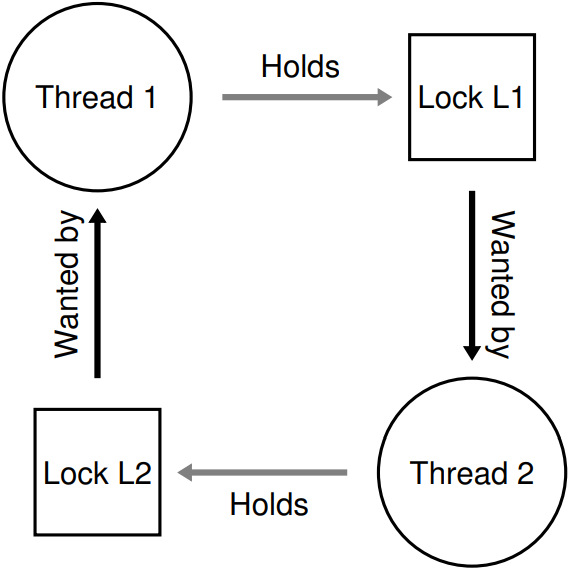
\includegraphics[width=\linewidth,height=3.6cm]{imgs/deadlocks1}
\end{minipage}
\section*{Reasons for Deadlock}
\begin{enumerate}
\item circular dependencies between threads and resources, such that none of the threads can acquire the required resources to make progress
\item encapsulation: modularity does not mesh well with locking
\end{enumerate}
\section*{4 must-hold conds for a deadlock to occur (any unmet, no deadlock)}
\begin{itemize}
\item \textbf{Mutual exclusion} Threads claim exclusive control of resources that they require (e.g. a thread grabs a lock)
\item \textbf{Hold-and-wait} Threads hold resources they already acquired (e.g. locks) while waiting for extra resources (locks they wish to acquire)
\item \textbf{No preemption} can't forcibly rm resources from $T$s holding them
\item \textbf{Circular wait} a circular chain of $T$s such that each $T$ holds one or more resources (e.g. locks) being requested by the next $T$ in the chain
\end{itemize}
\section*{Prevent circular wait $\to$ total/partial ordering on lock acquisition}
\begin{itemize}
\item if \emph{only} 2 locks (\texttt{L1},\texttt{L2}), strict ordering: always acquire \texttt{L1} before \texttt{L2}
\item lock acquisition must respect the partial ordering (reflexive, transitive, anti-symmetric) $\to$ guarantee no circularity
\end{itemize}
\begin{minipage}{0.5\linewidth}
\begin{lstlisting}[language=c,xleftmargin=2pt]
// fn need to grabs two locks
do sth(mutex t *m1, mutex t *m2)
\end{lstlisting}
  \begin{itemize}
  \item if always grabs \texttt{m1} before \texttt{m2} (or \texttt{m2} before \texttt{m1}) $\to$ may deadlock
  \item $\because T_1$ calls \texttt{do\_sth(m1, m2)} while $T_2$ calls \texttt{do\_sth(m2, m1)} $\to$ deadlock
  \item $T_1$ waits for \texttt{m2}; $T_2$ waits for \texttt{m1}
  \item fix: enforce ordering by lock addr
  \end{itemize}
\end{minipage}
\begin{minipage}{0.5\linewidth}
\begin{lstlisting}[language=c,xleftmargin=4pt,framextopmargin=1pt]
// grab in high-to-low addr order
if (m1 > m2) {
  pthread_mutex_lock(m1);
  pthread_mutex_lock(m2);
} else {
  pthread_mutex_lock(m2);
  pthread_mutex_lock(m1);
}
// assume m1 != m2 (not same lock)
\end{lstlisting}
\end{minipage}
\section*{Prevent hold-and-wait $\to$ acquire all locks at once, atomically}
\begin{minipage}{0.75\linewidth}
\begin{lstlisting}[language=c,xleftmargin=2pt]
pthread_mutex_lock(prevention); // begin acquisition
pthread_mutex_lock(L1);
pthread_mutex_lock(L2);
...
pthread_mutex_unlock(prevention); // end
\end{lstlisting}
\end{minipage}
\begin{minipage}{0.3\linewidth}
  \flushleft
  \begin{itemize}
  \item \mb{must} first grab \texttt{prevention} lock
  \item ensure no untimely $T$ switch can occurs $\to$ avoid deadlock
  \end{itemize}
\end{minipage}
\begin{itemize}
\item Ok for $T$ to acquire \texttt{L1}$\cdots$\texttt{L2} in any order $\because$ it already holding \texttt{L}$_\text{prevention}$
\item must know exactly which locks must be held and acquire ahead of time
\item concurrency $\downarrow$ $\because$ must acquire all locks at once even when not need to
\end{itemize}
\begin{minipage}{0.56\linewidth}
\section*{Add Preemption: imperfect, working}
\begin{lstlisting}[language=c,xleftmargin=2pt]
top:
  pthread_mutex_lock(L1);
  if (pthread_mutex_trylock(L2) != 0) {
    pthread_mutex_unlock(L1);
    goto top;
  }
\end{lstlisting}
\end{minipage}
\begin{minipage}{0.44\linewidth}
  \flushleft
  \begin{itemize}
  \item deadlock-free, ordering-robust lock acquisition protocol:
  \item try to grab lock if available $\to$ success
  \item if lock held by other $\to$ error; try again later
  \end{itemize}
\end{minipage}
\begin{itemize}
\item $T_{\text{other}}$ could follow same protocol but grab lock in order of \texttt{L2} then \texttt{L1}
\item this leads to \mo{livelock}: both systems running through this code sequence repeatedly (thus not a deadlock), but progress not being made
\item add a random delay before looping back and trying over again $\to$ decreasing the odds of repeated interference among competing threads
\item[1.] if \texttt{L1} gets dropped in some routine, go-back $\to$ more complex
\item[2.] if along \texttt{L1}, extra mem also acquired, must ensure to release mem too
\item[3.] \emph{not} really \emph{add} preemption, but just preempt its own lock ownership
\end{itemize}
\section*{Prevent Mutual Exclusion (lock-free data struct + hardware help)}
\begin{minipage}{0.5\linewidth}
\begin{lstlisting}[language=c]
int CompAndSwap(
  int *addr, int expected, int new
) {
  if (*addr == expected) {
    *addr = new;
    return 1; // success
  }
  return 0; // failure
} // atomic ix provided by hardware
\end{lstlisting}
\end{minipage}
\begin{minipage}{0.5\linewidth}
\begin{lstlisting}[language=c,xleftmargin=2pt]
void AtomicIncrement(
  int *val, int amt
) {
  do {
    int old = *val;
  } while (
  CompAndSwap(val, old, old + amt)
  == 0); // if val == old, inc old
} // else keep trying
\end{lstlisting}
\end{minipage}
livelock still possible; robust solution will be more complex than above\newline
\begin{minipage}{0.55\linewidth}
\section*{list insertion example}
\begin{lstlisting}[language=c,frame=none,xleftmargin=-6pt]
// thread-unsafe: race condition
void insert(int value) {
  node_t *n = malloc(sizeof(node_t));
  assert(n != NULL);
  n->value = value;
  n->next = head;
  head = n;
}
\end{lstlisting}
\end{minipage}
\begin{minipage}{0.5\linewidth}
\begin{lstlisting}[language=c,frame=none,xleftmargin=-18pt]
void insert(int value) {
  node_t *n = malloc(sizeof(node_t));
  assert(n != NULL);
  n->value = value;
  pthread_mutex_lock(listlock);
  n->next = head;
  head = n;
  pthread_mutex_unlock(listlock);
} // lock critical section
\end{lstlisting}
\end{minipage}
\begin{minipage}{0.68\linewidth}
\begin{lstlisting}[language=c]
void insert(int value) {
  node_t *n = malloc(sizeof(node_t));
  assert(n != NULL);
  n->value = value;
  do {
    n->next = head;
  } while (CompAndSwap(&head, n->next, n) == 0);
} // retry again with new head by other thread
\end{lstlisting}
\end{minipage}
\begin{minipage}{.32\linewidth}
  \flushleft
  \begin{itemize}
  \item point \texttt{next} to curr head and try to make the node new head
  \item this will fail if some other $T$ successfully swapped in a new head in meanwhile
  \item then try again
  \end{itemize}
\end{minipage}
\section*{Deadlock Avoidance via Scheduling}
\begin{minipage}{.4\linewidth}
  \begin{tabular}[ht]{lllll}
    Lock        & \texttt{T1} & \texttt{T2} & \texttt{T3} & \texttt{T4} \\
    \texttt{L1} & yes & yes & \mr{no} & no \\
    \texttt{L2} & yes & yes & yes & no \\
  \end{tabular}
\end{minipage}
\begin{minipage}{.6\linewidth}
  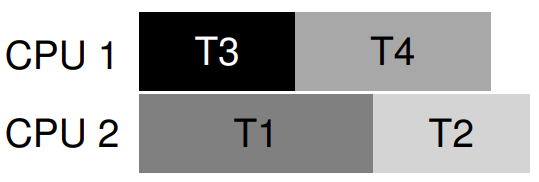
\includegraphics[width=.9\linewidth,height=1.8cm]{imgs/threadsdeadlock2}
\end{minipage}
\begin{itemize}
\item A smart scheduler could ensure T1 and T2 are not run at the same time $\to$ no deadlock could ever arise
\item  it is OK for (T3 and T1) or (T3 and T2) to overlap. Even
though T3 grabs lock \texttt{L2}, it can never cause a deadlock by running concurrently with other threads because it only grabs one lock
\end{itemize}
\begin{minipage}{.4\linewidth}
  \begin{tabular}[ht]{lllll}
    Lock        & \texttt{T1} & \texttt{T2} & \texttt{T3} & \texttt{T4} \\
    \texttt{L1} & yes & yes & \mr{yes} & no \\
    \texttt{L2} & yes & yes & yes & no \\
  \end{tabular}
\end{minipage}
\begin{minipage}{.6\linewidth}
  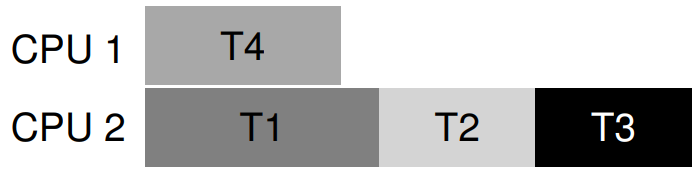
\includegraphics[width=\linewidth,height=1.8cm]{imgs/threadsdeadlock3}
\end{minipage}
\begin{itemize}
\item T1, T2, and T3 all need to grab both locks \texttt{L1} and \texttt{L2} at some point
\item static scheduling leads to conservative approach: T1, T2, T3 all run on same processor: $\to T_{\text{total-completion-time}} \uparrow$ considerably
\item deadlock avoidance: not a widely-used general-purpose solution
\end{itemize}
\section*{Detect and Recover}
\begin{itemize}
\item allow deadlocks to occasionally occur $\to$ reboot once detected it
\item this non-solution is indeed pragmatic if deadlocks are rare
\item Many DBMS employ deadlock detection and recovery techniques
\item deadlock detector runs periodically, building a resource graph and checking for cycles; when there's a cycle (deadlock), sys needs reboot
\end{itemize}
\begin{tcolorbox}[left=0mm, top=1mm, right=0mm, rightlower=0mm, bottom=1mm,
  title=USE ATOMIC OPERATIONS,
  halign title=center]
  The idea behind making a series of actions \textbf{atomic}: ``all or nothing''. It should either appear as if all of the actions you wish to group together occurred, or that none of them occurred, with no in-between state visible. Sometimes, the grouping of many actions into a single atomic action is called a \textbf{transaction}
\end{tcolorbox}
\begin{tcolorbox}[left=0mm, top=1mm, right=0mm, rightlower=0mm, bottom=1mm,
  title= DON'T ALWAYS DO IT PERFECTLY (TOM WEST'S LAW),
  halign title=center]
  ``Not everything worth doing is worth doing well'': If a bad thing happens rarely, certainly one should not spend much effort to prevent it, \emph{particularly if} the cost of the bad things is small. With pressing deadlines and other real-world concerns, one will always have to decide which aspects of a system to build well and which to put aside
\end{tcolorbox}

% \input{subs/ch33_iodevs}
% \section*{Hard Disk Drives Interface}
\begin{itemize}
\item consists of a large number of sectors (512-byte blocks): numbered from 0 to $n-1$ on a disk with $n$ sectors; each can be read and written
\item can be viewed as \texttt{array[n]} of sectors: 0 to $n-1$ (\textbf{address space})
\item OS typically read or write $\geq$ 4KB at a time; Hardware only guarantees a single 512-byte write is \textbf{atomic}
\item if untimely power loss occurs $\to$ only a portion of a large write may complete (aka \textbf{torn write})
\end{itemize}
\section*{Modern Disk Components (Basic Geometry)}
\begin{itemize}
\item \textbf{platter} a circular hard surface on which data is stored persistenly by inducing magnetic changes to it
  \begin{itemize}
  \item a disk may have $\geq$ 1 platter; each has 2 sides (called surface)
  \item platters usually made of hard material (aluminum), coated with thin magnetic layer to persistently store bits even when drive's powered off
  \end{itemize}
\item platters all bound to \textbf{spindle}, which is connected to motor that spins platters around (when powered on) at a constant/fixed rate
  \begin{itemize}
  \item The rotation rate often measured in rotations per minute (RPM), and typical modern values:  7,200 - 15,000 RPM
  \item often interested in the time of a single rotation: 10,000 RPM $\to$ a single rotation takes about 6ms (see right equations)
  \end{itemize}
\item Data is encoded on each surface in concentric circles of sectors (each such such concentric circle is called \textsc{track})
  \begin{itemize}
  \item A single surface contains thousands of tracks, tightly packed together
  \item hundreds of tracks fitting into the width of a human hair
  \end{itemize}
\item To read/write from the surface, need a mechanism to either sense (read) the magnetic patterns on the disk or to induce a change in (write) them
  \begin{itemize}
  \item This process of reading and writing is accomplished by the \textbf{disk head}
  \item there is one such head per surface of the drive
  \item The disk head is attached to a single \textbf{disk arm}; it moves across the surface to position the head over the desired track
  \end{itemize}
\end{itemize}
\begin{minipage}{.35\linewidth}
  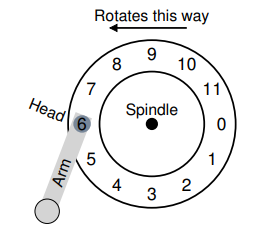
\includegraphics[width=\linewidth,height=3cm]{imgs/disk_stah}
\end{minipage}
\begin{minipage}{.65\linewidth}
  \flushleft
  \begin{itemize}
  \item must wait for desired sector to rotate under disk header; happens often in modern drives
  \item wait $\to$ key component of I/O service time, named \mb{rotational delay} (aka rotation delay)
  \item if full rotational delay is $R \to$ needs $\frac{R}{2}$ if stay at 6 and wait for 0 for read/write
  \item worse case: stay at 6 and wait for 5 $\to$ need full rotational delay $R$
  \end{itemize}
\end{minipage}
\begin{minipage}{.75\linewidth}
  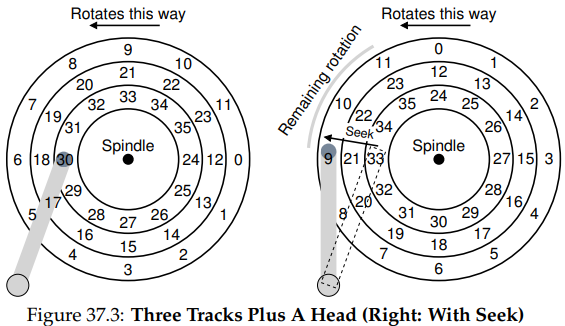
\includegraphics[width=\linewidth]{imgs/disk_3tracks}
\end{minipage}
\begin{minipage}{.25\linewidth}
  \flushleft
  \begin{itemize}
  \item head currently positioned over innermost track
  \item \mo{innermost} track: sectors 24-35
  \item \mo{middle} track: sectors 12-23
  \item \mo{outermost} track: sectors 0-11
  \item request a read to sector 11
  \item steps shown $\downarrow$
  \end{itemize}
\end{minipage}
\begin{enumerate}
\item drive moves disk arm to correct track (outermost) in a process (\mb{seek})
\item \textbf{seek} (one of most costly disk ops) has many phases
  \begin{itemize}[leftmargin=.1em]
  \item \emph{acceleration}: disk arm gets moving
  \item \emph{coasting} disk arm moves at full speed
  \item \emph{deceleration} disk arm slows down at full speed
  \item \emph{settling} disk head positioned over correct track: $T_{\text{settling}} = 0.5 \sim 2$ms
  \end{itemize}
\item[] during the seek, platter has rotated, in this case about 3 sectors. Thus, sector 9 is just about to pass under disk head, and we must only endure a short rotational delay to complete the transfer
\item \textbf{transfer}: sector 11 passes under disk head and data read/written to/from the surface; usually $T_{\text{transfer}} < T_{\text{seek}}$ and $T_{\text{transfer}} < T_{\text{rotation}}$
\end{enumerate}
\begin{minipage}{.45\linewidth}
  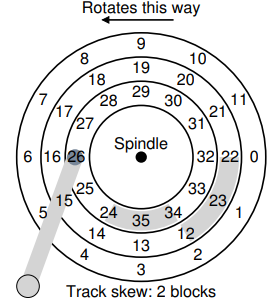
\includegraphics[width=\linewidth]{imgs/disk_trackskew}
\end{minipage}
\begin{minipage}{.55\linewidth}
  \flushleft
  \begin{itemize}
  \item \mb{track skew} rearrange sectors to ensure sequential reads to be properly served even when crossing track boundaries
  \item w/t skew, head would be moved to next track but the desired next block would've already rotated under head $\to$ wait almost full rotational delay
  \item outer tracks have more space $\to$ more sectors (\mo{multi-zoned} disk drives)
  \item \mb{cache} (track buffer) t some small amount of memory (usually around 8 or 16 MB) which drive uses to hold data read from or written to disk
  \item \mb{write back} data $\to$ cache
  \item \mb{write through} data $\to$ disk
  \end{itemize}
\end{minipage}
\begin{itemize}
\item Write back somets makes drive appear ``faster'', but can be dangerous
\item  if file sys/apps require that data be written to disk in certain order for correctness, write-back caching can lead to problems (see journaling)
\item 10K RPM disk, each rotation takes ? milliseconds (1)
\item 100 MB/second disk, to transfer 512 KB block in ? milliseconds (2)
\end{itemize}
\[
  \frac{Time(ms)}{1\;Rot.} = \frac{1\;\cancel{minute}}{10,000\;Rot.}\cdot \frac{60\; \cancel{second}}{1\;\cancel{minute}}\cdot \frac{1000\;ms}{1\;\cancel{second}} = \frac{60,000\;ms}{10,000\;Rot.} = \frac{6\;ms}{Rotation}
\]
\[
  \frac{Time(ms)}{1\;Request.} = \frac{512\;\cancel{KB}}{1\;Request}\cdot \frac{1\;\cancel{MB}}{1024\;\cancel{KB}}\cdot \frac{1\;\cancel{second}}{100\;\cancel{MB}}\cdot \frac{1000\;ms}{1\;\cancel{second}} = \frac{5\;ms}{Request}
\]
\section*{I/O Time Calculation}
\begin{itemize}
\item average I/O time calculation: $T_{I/O} = T_{seek} + T_{rotation} + T_{transfer}$
\item average time of data transfer: $R_{I/O} = \frac{Size_{transfer}}{T_{I/O}}$
\item \textbf{random}: read/write small (4KB) to random locations on disk (DBMS)
\item \textbf{sequential}: read/write a large number of consecutive sectors from disk
\item Cheetah: ``high performance'' drive market, spin as fast as possible, low seek times, and transfer data quickly
\item Barracuda: ``capacity'' market, cost per byte matters most $\to$ slower but pack as many bits as possible into the space available
\end{itemize}
\begin{minipage}{.5\linewidth}
  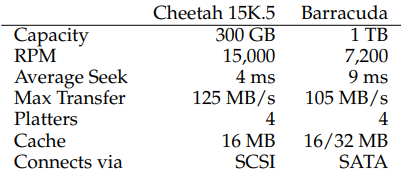
\includegraphics[width=\linewidth]{imgs/disk_scsivssata}
\end{minipage}
\begin{minipage}{.5\linewidth}
  \flushleft
  \begin{itemize}
  \item $T_{trans-Ch} = \frac{4KB}{125MB/s} \approx 32\; \mu\text{s}$
  \item $T_{trans-Ba} = \frac{4KB}{105MB/s} \approx 38\; \mu\text{s}$
  \item $1\;\text{ms} = 1000\; \mu\text{s}$
  \end{itemize}
  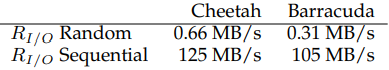
\includegraphics[width=\linewidth]{imgs/disk_scsivssata1}
\end{minipage}
\begin{enumerate}
\item there is a huge gap in drive performance between random and sequential workloads: $\approx 200$ for the Cheetah and $\approx 300+$ for Barracuda
\item there is a large difference in performance between high-end ``performance'' drives (expensive) and low-end ``capacity'' drives (cheap)
\end{enumerate}
\begin{tcolorbox}[left=0mm, top=1mm, right=0mm, rightlower=0mm, bottom=1mm,
  title= Use Disks Sequentially,
  halign title=center]
  When at all possible, transfer data to/from disks in a sequential manner. If that is not possible, at least try to transfer data
in large chunks: the bigger, the better. If I/O is done in little random
pieces, I/O performance will suffer dramatically. Also, users will suffer.
\end{tcolorbox}
\begin{itemize}
\item Scheduling algorithms for CPU time are also useful for I/O
\end{itemize}
\section*{Disk Scheduling: shortest job first (SJF principle)}
\begin{itemize}
\item disk scheduler can estimate seek and rotational delay of a disk request
\item (greedily) pick the one that will take the least time to service first
\end{itemize}
\begin{minipage}{.25\linewidth}
  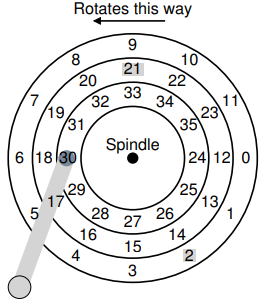
\includegraphics[width=\linewidth]{imgs/disk_sstf}
\end{minipage}
\begin{minipage}{.75\linewidth}
  \flushleft
  \begin{itemize}
  \item shortest-seek-(time)-first (SS(T)F) orders queue of I/O requests by track, picking those on the nearest track to complete first
  \item $P_{\text{head}}$ over inner track: request 21[mid] or 2[outer]?
  \item request \textbf{21} first; when it completes; \emph{then} request \textbf{2}
  \item Position of disk head relative to the requested position matters \emph{more}
than length of the transfer
  \end{itemize}
\end{minipage}
\begin{enumerate}
  \item drive geometry (\texttt{array[n]} of sectors) \mr{invisible} to OS $\to$ OS uses \mo{nearest-block-first} (NBF) to sched reqs with nearest block addr next
  \item \mr{starvation}: steady stream of reqs to inner track (current head pos) $\to$ Requests to other tracks be ignored completely due to pure SSTF
\end{enumerate}
\section*{Elevator (SCAN, F-SCAN, C[ircular]-SCAN) $\to$ prevent starvation}
\begin{enumerate}
\item \textbf{SCAN} moves back/forth across disk serving reqs in order across tracks $\to$ passing through middle twice before back to outer again
  \begin{itemize}[leftmargin=.1em]
  \item \mb{sweep} a single pass across disk (outer $\to$ inner or inner $\to$ outer)
  \item requests on already-serviced track in this sweep will be queued until the next sweep (in the other direction)
  \end{itemize}
\item \textbf{F-SCAN} freezes the queue to be serviced when doing a \emph{sweep}
    \begin{itemize}[leftmargin=.1em]
  \item places reqs coming in during the sweep into queue to be served later
  \item avoids starvation of far-away requests, by delaying the servicing of late-arriving (but nearer by) requests
  \end{itemize}
\item \textbf{C-SCAN} only sweeps from outer-to-inner, and then resets at the outer track to begin again $\to$ a bit more fair to inner and outer tracks
\item[] SCAN and its cousins \texttt{!=} the best scheduling tech:
  \begin{enumerate*}[label={\alph*},font={\color{red!50!black}\bfseries}]
  \item not actually adhere as closely to the principle of SJF as they could;
  \item ignore rotation
  \end{enumerate*}
\end{enumerate}
\section*{Shortest Positioning Time First (SPTF)}
\begin{minipage}{.3\linewidth}
  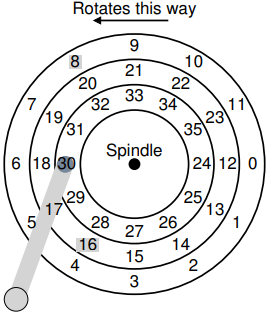
\includegraphics[width=\linewidth]{imgs/disk_sstf1}
\end{minipage}
\begin{minipage}{.7\linewidth}
  \flushleft
  \begin{itemize}
  \item scheduler has to decide: sched \textbf{16} or \textbf{8} for next?
  \item depends on relative time of seeking and rotation
  \item if $T_{\text{seek}} \gg T_{\text{rot.}} \to$ SSTF (or variants) are fine
  \item if $T_{\text{seek}} \ll T_{\text{rot.}} \to$ seek \textbf{further} to service request 8 on outer track \emph{better} than seek to service 16 on middle track (almost full rotation)
  \item On modern drives $T_{\text{seek} \approx T_{\text{rot.}}} \to$ SPTF is useful
  \item OS knows little about track boundaries and disk current head position (in rotational sense), $\to$ SPTF is usually performed inside a drive
  \end{itemize}
\end{minipage}
\begin{itemize}
\item older OS did all the scheduling: check pending requests, pick the best one, issue it to the disk. When that request completed, sched next one
\item modern disk drives have sophisticated internal schedulers (inside disk controller, all relevant details available, including exact $Pos_{\text{head}}$):
  \begin{enumerate}[leftmargin=.2em]
  \item OS scheduler issues what it thinks the best few requests all to disk
  \item disk uses its internal knowledge of $Pos_{\text{head}}$ and detailed track layout info to service said requests in the best possible (SPTF) order
  \item \mb{I/O merging} adjacent reqs on same track (eg 33, 34) will be merged; important at OS level $\because$ requests number to disk $\downarrow \to$ overheads $\downarrow$
  \item immediately issue req to drive (\mo{work-conserving}) $to$ disk never idle
  \item \mo{non-work-conserving}: wait for new/ better req to arrive $\to$ overall efficiency $\uparrow$ (deciding when to wait \& for how long can be tricky)
  \end{enumerate}
\end{itemize}
\section*{Linux Completely Fair Queueing (CFQ) scheduler}
\begin{itemize}
\item queue for each process; yield slice only if idle for given time
\item weighted RR between queues with slice-time proportional to priority
\item CFQ replaced by Budget Fair Queuing (BFQ)
\item other Linux scheduler:
  \begin{enumerate*}[label={\alph*},font={\color{red!50!black}\bfseries}]
  \item \texttt{noop} first come first serve.
  \item \texttt{deadline} impose a ``deadline'' on each I/O req to avoid starvation
  \end{enumerate*}
\end{itemize}

% \section*{Creating Files (\texttt{open} system call)}
\begin{lstlisting}[language=c]
// new: `open' also create a file if it doesn't exist yet
int fd = open("foo", O_CREAT|O_WRONLY|O_TRUNC, S_IRUSR|S_IWUSR);
// old: equivalent to calling open() with O_CREAT | OWRONLY | O_TRUNC
int fd = creat("foo"); // option: add second flag to set permissions
\end{lstlisting}
Flags and parameters:
\begin{enumerate*}[label={\alph*.},font={\color{red!50!black}\bfseries}]
\item \texttt{O\_CREAT} creates the file if it doesn't exit
\item \texttt{O\_WRONLY} ensures it can only be written to and
\item if the file already exits, truncate it to a size of zero bytes $\to$ removing any existing content (\texttt{O\_TRUNC})
\end{enumerate*}
The 3rd parameter specifies permissions, making the file readable and writable by the owner. On success, return a \mb{file descriptor}\\
\begin{minipage}{.45\linewidth}
\begin{lstlisting}[language=c]
struct proc {
  // other fields ...
  // array of open file
  struct file *ofile[NOFILE];
  // other fields ...
} // Linux uses task_struct
\end{lstlisting}
\end{minipage}
\begin{minipage}{.55\linewidth}
  \flushleft
  \begin{itemize}
  \item xv6 keeps an \texttt{array[NOFILE] of files}, indexed by file descriptor
  \item tracks which files are opened on a per-process basis
  \item each entry a ptr to a \texttt{struct file} to track the file being read/written
  \end{itemize}
\end{minipage}
\section*{Reading \texttt{read()} and Writing \texttt{write()} files (sequentially: start $\to$ end)}
\begin{lstlisting}[language=bash]
# run strace cat foo in terminal; get below output (relevant only)
# O_LARGEFILE -> 64-bit offset; 3 -> returned file descriptor
open(``foo'', O_RDONLY|O_LARGEFILE) = 3
# read fd 3 into buffer ``hello\n'' of size 4KB; returned bytes read: 6
read(3, ``hello\n'', 4096)              = 6
# `cat' may call `write' or `printf' which `write' to stdout (1)
write(1, ``hello\n'', 6)                = 6 # write to stdout
hello
read(3, ``'', 4096)                     = 0 # nothing to read, returns 0
close(3)                                = 0 # indicate done
\end{lstlisting}
Writing a file in similar steps:
\begin{enumerate*}[label={\alph*.},font={\color{red!50!black}\bfseries}]
\item a file is opened for writing,
\item then call \texttt{write()} syscall, perhaps repeatedly for larger files,
\item then \texttt{close()}
\end{enumerate*}
\section*{Reading/Writing not sequentially (current offset updated in 2 ways)}
\begin{lstlisting}[language=c]
// look up specific word -> read from random offsets within a file
off_t lseek(int fildes, off_t offset, int whence);
// If whence is SEEK_SET, the offset is set to offset bytes.
// If whence is SEEK_CUR, offset = its current location + offset bytes
// If whence is SEEK_END, offset = file size + offset bytes
\end{lstlisting}
\begin{enumerate}
\item \emph{explicitly} with \texttt{lseek}, which changes the offset as specified above
\item when R/W of $N$ bytes, \texttt{curr\_offset += N}: \emph{implicitly} updates offset
\end{enumerate}
\begin{minipage}{.3\linewidth}
\begin{lstlisting}[language=c]
struct file {
  int ref; // sharing
  char readable;
  char writable;
  struct inode *ip;
  uint off;
}; // simplified def
\end{lstlisting}
\end{minipage}
\begin{minipage}{.7\linewidth}
  \flushleft
  \begin{itemize}
  \item OS uses this to determine whether opened file is readable or writable or both
  \item \texttt{struct inode ip} points to the underlying file
  \item These file structs represent all of the currently opened files in the system; together, they are sometimes referred to as the \mb{open file table}
  \end{itemize}
\end{minipage}
\begin{minipage}{.45\linewidth}
\begin{lstlisting}[language=c]
struct {
  struct spinlock lock;
  struct file file[NFILE];
} ftable;
\end{lstlisting}
\end{minipage}
\begin{minipage}{.55\linewidth}
  \flushleft
  \begin{itemize}
  \item open file table keeps \texttt{struct file}
  \item in most cases, there's 1-to-1 mapping from \texttt{fd} to an entry in OFT, but it may be shared
  \end{itemize}
\end{minipage}
\begin{itemize}
\item mutil procs read same file at same timw: each has its own OFT entry
\item each logical R/W of a file is independent, with its own current offset
\end{itemize}
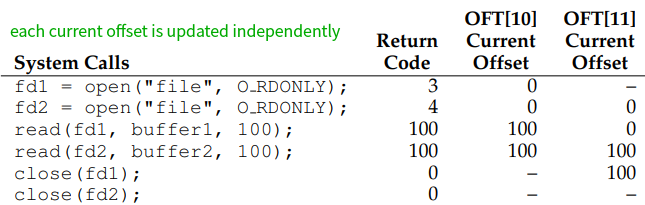
\includegraphics[width=\linewidth]{imgs/fs_read_conc}
\section*{Shared File Table Entries \texttt{fork} and \texttt{dup}}
\begin{minipage}{.4\linewidth}
  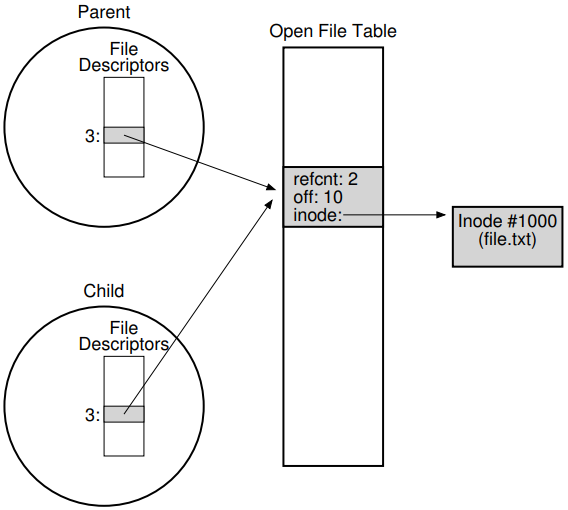
\includegraphics[width=\linewidth]{imgs/fs_shared_ote}
\end{minipage}
\begin{minipage}{.6\linewidth}
  \flushleft
  \begin{itemize}
  \item when parent process \texttt{fork()} a child, child shares its parent's OTF
  \item each process has its own independent copy of file descriptor
  \item \texttt{ref} in \texttt{struct file} keeps \# descriptors sharing the entry; only when both processes close file (or exit) will the entry be removed
  \item \texttt{dup()} creates new fd that refers to same OFT entry (file) as an existing fd
  \end{itemize}
\end{minipage}
\section*{Writing Immediately \texttt{fsync()}}
\begin{itemize}
\item  For performance reasons, the file system may \textbf{buffer} \texttt{write()} to memory for a short while before actually writing it to disks
\item  Drawback: some writes may be lost if the system crashes (power loss); DBSM recovery protocol may require ability to force write to disk
\item syscall \texttt{fsync()} tells file system to force writing all \textbf{dirty} data to disk
\item May need to \texttt{fsync()} both a file and the directory containing it
\end{itemize}
\begin{itemize}
\item Another method to R/W a file: map it to memory using syscall \texttt{mmap()}
\item R/W to a file becomes load/store to its memory-mapped locations
\item \texttt{msync()} to flush changes in memory to the file system
\item Key benefits:
\begin{enumerate*}[label={\alph*.},font={\color{red!50!black}\bfseries}]
\item creates a direct link btwn file byte offsets (backing file) and virtual addr in calling process
\item combines file persistence and memory-like access semantics;
\item enables persistent memory programming;
\item Makes apps faster by avoiding RAM-disk data changes
\end{enumerate*}
\end{itemize}
\section*{Renaming Files: \texttt{rename()} (atomic operation during sys crashes)}
\begin{itemize}
\item on command line: \texttt{mv}; use syscall \texttt{rename(char *old, char *new)}
\item file will have either old or new name; \emph{no} partial states possible
\item common file update process:
  \begin{enumerate*}[label={\alph*.},font={\color{red!50!black}\bfseries}]
  \item write new content to tmp file;
  \item sync temp file to disk;
  \item rename tmp file to target (used by text editors)
  \end{enumerate*}
\begin{lstlisting}[language=c]
int fd = open("foo.txt.tmp", O_WRONLY|O_CREAT|O_TRUNC,
              S_IRUSR|S_IWUSR);
write(fd, buffer, size); // write out new version of file
fsync(fd); close(fd); rename("foo.txt.tmp", "foo.txt");
\end{lstlisting}

\item key benefits:
  \begin{enumerate*}[label={\alph*.},font={\color{red!50!black}\bfseries}]
  \item ensures atomic updates
  \item prevents data loss
  \item old file remains until update complete (for safe file modifications)
  \end{enumerate*}
\end{itemize}
\section*{Getting Info About Files \texttt{stat()} and Remove (\texttt{unlink()} syscall)}
\begin{minipage}{.7\linewidth}
\begin{lstlisting}[language=c]
struct stat {
  dev_t st_dev; // ID of device containing file
  ino_t st_ino; // inode number
  mode_t st_mode; // protection
  nlink_t st_nlink; // number of hard links
  uid_t st_uid; // user ID of owner
  gid_t st_gid; // group ID of owner
  dev_t st_rdev; // device ID (if special file)
  off_t st_size; // total size, in bytes
  blksize_t st_blksize; // blksize for filesys I/O
  blkcnt_t st_blocks; // number of blks allocated
  time_t st_atime; // time of last access
  time_t st_mtime; // time of last modification
  time_t st_ctime; // time of last status change
};
\end{lstlisting}
\end{minipage}
\begin{minipage}{.3\linewidth}
  \flushleft
  \begin{itemize}
  \item metadata keeps info on each file in sys
  \item accessed via \texttt{stat()} and \texttt{fstat()}
  \item takes pathname and fd as input
  \item inode struct:
    \begin{enumerate*}[label={\alph*.},font={\color{red!50!black}\bfseries}]
    \item stored persistently on disk
    \item active inodes cached in RAM to speed up access
    \item acts as fs's data struct
    \end{enumerate*}
  \end{itemize}
\end{minipage}
\section*{Directory Syscalls for Making, Reading, Deleting Directories}
\begin{itemize}
\item dirs format is fs metadata $\to$ user can’t modify its bytes arbitrarily
\item updates \emph{only} through \mr{indirect} actions:
  \begin{enumerate*}[label={\alph*.},font={\color{red!50!black}\bfseries}]
  \item \texttt{mkdir}
  \item \texttt{opendir}
  \item \texttt{rmdir}
  \item \texttt{readdir} to read dir entries (files, subdirs)
  \item \texttt{closedir}
  \end{enumerate*}
\item \texttt{rmdir()} requires the dir to be empty: only has \texttt{.} and \texttt{..} before deleting it $\to$ removing non-empty causes \texttt{rmdir()} to fail
\item dirs are light on info: just mapping name to inode number, plus a few other details $\to$\ texttt{ls -l} calls \texttt{stat()} on each file to get more info
\end{itemize}
\begin{lstlisting}[language=c]
struct dirent {
  char d_name[256];           // filename
  ino_t d_ino;                // inode number
  off_t d_off;                // offset to the next dirent
  unsigned short d_reclen; // length of this record
  unsigned char d_type;       // type of file
};
\end{lstlisting}
\section*{Hard, Soft links with \texttt{link()} and \texttt{unlink()}}
\begin{itemize}
\item \texttt{ln} uses \texttt{link()} syscall that takes two args: old and new pathnames
\item \mo{link} creates a new file name to refer to the old, existing one (not copied in any way, just two human-readable names referring to the same file)
\item creating a file is doing two things:
  \begin{enumerate*}[label={\alph*.},font={\color{red!50!black}\bfseries}]
  \item make inode struct that tracks all relevant info about the file (size, blk location on disk, etc)
  \item \emph{link} a human-readable name to that file and put that link into a directory
  \end{enumerate*}
\item file system see no difference between original and new files
\item Each inode keeps a \mb{reference count} (link count) to track how many file names associated with it
\item \texttt{unlink()} removes ``link'' btwn human-readable name and inode number, decrements ref count $\to$ iif \texttt{ref\_cnt == 0}, fs truly deletes the file
\item \textbf{can't} hard link to a directory (for fear of cycle in directory tree)
\item \textbf{can't} hard link to files on other disk partitions $\because$ inode numbers only unique within a particular file system, not across file systems
\end{itemize}
\begin{lstlisting}[language=bash]
prompt> echo hello > file           # create a file with some content
prompt> stat file                   # use `stat' to see the reference count
... Inode: 67158084 Links: 1 ...
prompt> ln file file2               # hard link to an existing file
prompt> stat file
... Inode: 67158084 Links: 2 ...  # reference count incremented by 1
\end{lstlisting}
\begin{itemize}
\item symbolic (soft) link is a file itself of a different type (not \texttt{-} or \texttt{d}, but \texttt{l})
\item soft links \emph{only} refers to filename, \texttt{file\_size == bytes of filename}
\item shorter pathname $\to$ small soft link file, longer pathname $\to$ larger file
\item \mr{dangling reference}: removing original file causes soft link to points to pathname that no longer exists
\end{itemize}
\section*{Access Control encoded in Permission Bits}
\begin{itemize}
\item \textbf{3} groups of 3-bit data, controlling \textbf{r}ead/\textbf{w}rite/e\textbf{x}ecute access
\begin{lstlisting}[language=bash]
prompt> ls -l foo.txt
-rw-r--r-- 1 remzi wheel 0 Aug 24 16:29 foo.txt
# -: regular file; d: directory; l: symbolic link
\end{lstlisting}
\item one more extra group of 3-bit for setuid/setgid bits
\begin{lstlisting}[language=bash]
# setuid (0o4000): file owner; setgid (0o2000); sticky bit (0o1000)
chmod 4755 myfile  # Sets setuid and rwxr-xr-x
\end{lstlisting}
\item for directories, its execute bit enables a user (or group/others) to \texttt{cd} into the given directory and if with writable bit, create files therein
\end{itemize}
\begin{minipage}{.5\linewidth}
  \includegraphics[width=\linewidth]{imgs/file_perm2}
\end{minipage}
\begin{minipage}{.5\linewidth}
  \includegraphics[width=\linewidth]{imgs/file_perm1}
\end{minipage}
\section*{Making and Mounting A File System}
\begin{itemize}
\item \texttt{mkfs} accepts a device (e.g. \texttt{/dev/sda1}) and a fs type (e.g. \texttt{ext4}) $\to$ creates an empty fs starting with root dir onto that disk partition
\item \texttt{mount} (uses syscall \texttt{mount()}) takes an existing directory as a target \textbf{mount point} and essentially pastes a new fs onto the directory tree at that point, making new fs accessible within the uniform fs tree $\to$ unifies all file systems into one tree $\to$ uniform and convenient naming
\item run \texttt{mount} to see what is mounted and at which points on your sys
\end{itemize}

% \section*{Two key aspects of file system (data structures \& access methods)}
\includegraphics[width=\linewidth]{imgs/fs_simple_blocks1}
\begin{itemize}
\item divide disk into \textbf{blocks}: each of size 4KB, addressed from 0 to $N-1$
\item assume $N=64$ and low-level R/W ops on blocks already implemented
\item \textbf{data region}: region of disk used for user data; assume $N_{\text{data}} = 56$
\item assume $N_{\text{inode}}=5$ and $S_{\text{inode}}=256$B $\to$ 4KB block holds 16 inodes and fs contains 80 in total (max \# of files can be stored in this fs)
\item fs should have
  \begin{enumerate*}[label={\alph*.},font={\color{red!50!black}\bfseries}]
  \item data bloks (D)
  \item inodes (I)
  \item \mb{allocation structures}: bitmap(d,i) for D,I $\to$  free: 0; in-use: 1 (a bit overkill in this case)
\end{enumerate*}
\item \textbf{S}uperblock contains info:
  \begin{enumerate*}[label={\alph*.},font={\color{red!50!black}\bfseries}]
  \item $N_{\text{inodes}}=80; N_{\text{data}} = 56$
  \item inode table begins at block3
  \item magic number (enum) of fs type (vsfs)
  \item other info
\end{enumerate*}
\end{itemize}
\includegraphics[width=\linewidth]{imgs/fs_simple_blocks2}
\includegraphics[width=\linewidth]{imgs/fs_simple_blocks2}
\begin{itemize}
\item each inode implicitly pointed to by i-number (low-level name of a file)
\item inode table starts at 12KB and $S_{\text{indtb}} = 20$KB (5 4KB blocks)
\item disks are \emph{not} byte addressable but sector (e.g. 512B) addressable
\begin{lstlisting}[language=c,framextopmargin=-2pt,framexbottommargin=-2pt]
blk = (inumber * sizeof(inode_t)) / blockSize;
sector = ((blk * blockSize) + inodeStartAddr) / sectorSize;
\end{lstlisting}
\item metadata inside each inode:
  \begin{enumerate*}[label={\alph*.},font={\color{red!50!black}\bfseries}]
  \item type (\texttt{-,d,l})
  \item size (\# of blks allocated)
  \item protection info (ownership, access)
  \item time info, etc
\end{enumerate*}
\item each \mo{inode} can contain $\geq 1$ \mb{direct pointers} (disk addresses); each pointer refers to one disk block that belongs to the file
\item drawback: cannot support very large file $\because S \leq S_{\text{blk}} \times$ \texttt{num\_direct\_ptr}
\end{itemize}
\section*{Multi-level Index to support bigger files}
\begin{itemize}
\item \mb{indirect pointer} points to indirect blk containing more ptrs: each points to usr data: an inode with fixed \# of direct ptrs + 1 indirect ptr
\item If a file grows large enough, an indirect blk allocated (from data region) and the inode’s slot for an indirect pointer is set to point to it
\item assume 4KB block and 4B disk addr $\to N_{\text{ptr/blk}} = \frac{4KB}{4B} = 1024$
\item a file can grow to be $(12 + 1024) \cdot 4K = 4144KB$
\item \mb{double indirect pointer} refers to a block that contains pointers
to indirect blocks, each of which contain pointers to data blocks $\to$ files can grow to $(12 + 1024 + 1024^{2}) \times 4KB \approx 4GB$
\item \mb{triple indirect pointer} points to a blk that contains double indirect ptrs
\end{itemize}
\begin{minipage}{.5\linewidth}
  \includegraphics[width=\linewidth]{imgs/fs_indirect_ptr1}
\end{minipage}
\begin{minipage}{.5\linewidth}
  \includegraphics[width=\linewidth]{imgs/fs_indirect_ptr2}
\end{minipage}
\includegraphics[width=\linewidth]{imgs/fs_measure_sum}
\begin{itemize}
\item most files are small $\to$ can optimize the imbalanced tree (left)
\item typical inode has 12 dirct ptrs + $\geq 1$ indirect blocks for larger files
\end{itemize}
\section*{Directory Organization}
\begin{itemize}
\item filsys treats dirs as special type of file (\texttt{d}): represented in same way as files, with data blks pointed to by inode and perhaps indirect blks
\item XFS uses B-tree, faster than lists, file/dir name must be unique
\item simple org: a dir contains a list of (entry name, inode number) pairs
\item dir has a str + a number in data blks: each str may have variable len
\item
\end{itemize}
\begin{tabular}{l|l|l|l|l}
  inum & reclen & strlen  & name        & note \\
  5    & 12     &  2      & \texttt{.}  & (current dir)\\
  2    & 12     &  3      & \texttt{..} & (parent dir)\\
  12    & 12     &  4      & \texttt{foo}&\\
  13    & 12     &  4      & \texttt{bar}&\\
  24    & 36     & 28      & \texttt{foobar\_is\_a\_pretty\_longname}&\\
  \multicolumn{5}{l}{record len: total bytes for the name + any leftover space (`$\backslash$0' included)}\\
  \hline
  \multicolumn{5}{l}{deleting a file $\to$ empty space in middle of dir and should be marked}\\
  \multicolumn{5}{l}{new entry reuses old, bigger entry $\therefore$ extra space within and reclen is used}\\
\end{tabular}
\section*{Access Paths: Reading and Writing (assume filesize 12KB, blksize 4KB)}
\includegraphics[width=\linewidth, height=5.5cm]{imgs/fs_read_timeline}
\begin{itemize}
\item issue \texttt{open("/foo/bar",O\_RDONLY)} $\to$ filesys needs to find inode for \texttt{bar}
\item filesys only knows \mo{root} inumber: 2 by default; must \mo{traverse} pathname
\item read into root, find ptrs to data blocks, look for \texttt{foo} entry inumber
\item recursively traverse until desired inode found $\to$ \texttt{bar} inode into RAM
\item Once open, \texttt{read()} starts at offset 0 unless \texttt{lseek()} already called
\item read 1st block \& update
  \begin{enumerate*}[label={\arabic*.},font={\color{red!50!black}\bfseries}]
  \item $T_{\text{last-accessed}}$
  \item RAM OFT for this fd
  \item file offset $\to$ next read will read the second file block
  \end{enumerate*}
\item \texttt{close()}, deallocated fd, no disk I/O for closing file in this case
\item amount of I/O by open is \mr{proportional} to the length of the pathname
\item must read inode and data for each additional directory in the path
\item large dirs: read many data blks to find target entry $\to$ perfermance $\downarrow$
\item \texttt{open()} and \texttt{write()} $\to$ may allocate new block (unless overwriting)
\item each write
  \begin{enumerate*}[label={\arabic*.},font={\color{red!50!black}\bfseries}]
  \item decide which blk to alloc to the file, update other disk struct (bitmap, inode, etc)
  \item write data to disk
  \end{enumerate*}
\item 1 write $\to$ 5 I/Os:
  \begin{enumerate*}[label={\arabic*.},font={\color{red!50!black}\bfseries}]
  \item read bitmap; mark new alloc
  \item write new bitmap back to disk
  \item 2 more: read and write the inode
  \item write actual block
  \end{enumerate*}
\item create file: \textbf{10} I/Os and each alloc causes \textbf{5} I/Os:
  \begin{enumerate*}[label={\arabic*.},font={\color{red!50!black}\bfseries}]
  \item a pair to read/update the inode
  \item a pair to read/update the bitmap
  \item write data
  \end{enumerate*}
\end{itemize}
\includegraphics[width=\linewidth, height=7.5cm]{imgs/fs_write_timeline}
\section*{Caching and Buffering (modern filesys buffer Ws in RAM for 5-30s)}
\begin{itemize}
\item fixed-size cache to hold popular blocks and LRU to decide to keep which
\item fixed-size cache usually allocated at boot time; $\approx 10\%$ of total RAM
\item \mb{static partitioning}: wasteful, unable to re-purpose unused space; ensures each user receives some share of resource, usually delivers more predictable performance, often easier to implement
\item modern OS: \mb{dynamic partitioning} + virtual RAM: unified page cache; better utilization (by letting resrc-hungry users consume otherwise idle resrc); more complex to implement; can lead to worse perf. if one's idle resrc get consumed by others and need to take long time to reclaim
\item 1st open causes many I/Os; subsequent same file/dir opens hit cache
\item write has to put data to disk (persistent) so cache no longer serves
\item buffering write has benefits:
  \begin{enumerate*}[label={\arabic*.},font={\color{red!50!black}\bfseries}]
  \item filesys can batch updates into smaller set of I/Os: create file1 and later create file2 $\to$ update inode bitmap only once
  \item buffering writes in RAM $\to$ sys can schedule subsequent I/Os $\to$ perfermance $\uparrow$
  \item avoid some unnecessary writes: create a file and then delete it $\to$  avoid them entirely and lazy is good
  \end{enumerate*}
\item if sys crashes before actual writing data to disk, updates lost
\item DBMS usually forces writes to disk (\texttt{fsync()}, direct I/O interface)
\end{itemize}
\begin{tcolorbox}[left=0mm, top=1mm, right=0mm, rightlower=0mm, bottom=1mm,
  title= Reads DON’T access allocation structures,
  halign title=center]
  Allocation structures, such as bitmaps, are only accessed when allocation is needed. The inodes, directories, and indirect blocks have \emph{all} the information they need to complete a read request; there is no need to make sure a block is allocated when the inode already points to it.
\end{tcolorbox}
There needs to be some info about each file (metadata), usually
stored in a struct called an inode. Directories are just a specific type
of file that store name$\to$inode-number mappings. Filesys often use a bitmap to track which inodes/data blks are free/allocated.

% \section*{Disk-unware (list) filesys has poor performance}
\begin{itemize}
\item Thompson wrote the 1st simple filesys for Unix: \textbf{S}uperblock with info about entire filesys and most disk space taken up by data blocks
\item support files and directory-based hierarchy, easy-to-use
\item terrible performance: 2\% of overall disk bandwidth; worse over time
\end{itemize}
\begin{minipage}{.5\linewidth}
  \includegraphics[width=\linewidth]{imgs/ffs_list1}
\end{minipage}
\begin{minipage}{.5\linewidth}
  \includegraphics[width=\linewidth]{imgs/ffs_list2}
\end{minipage}
\begin{minipage}{.5\linewidth}
  \includegraphics[width=\linewidth]{imgs/ffs_list3}
\end{minipage}
\begin{minipage}{.5\linewidth}
  \includegraphics[width=\linewidth]{imgs/ffs_list4}
\end{minipage}
\begin{itemize}
\item main issue: treat disk like RAM; data spread all over the place; expensive positioning costs: data blks far away from its inode $\to T_{\text{seek}} \uparrow$
\item fragmentation: logically contiguous file accessed across the disk
\item defragmentation tools reorganize on-disk data to place files contiguously and make free space for $\geq 1$ contiguous regions
\item another issue: original block size too small (512 bytes) $\to$ transferring data from the disk was inherently inefficient: smaller blks minimizes internal fragement but bad for transfer $\because$ positioning overhead
\end{itemize}
\section*{FFS: Disk-Aware, Cylinder/Blk Groups (same API, diff. internal)}
\includegraphics[width=\linewidth]{imgs/ffs_cylinder}
\begin{itemize}
\item FFS keeps same interface/APIs: \texttt{open()},\texttt{read()}, \texttt{write()}, \texttt{close()}, etc
\item disk divided into cylinder groups: A single \mb{cylinder} is a set of tracks on different surfaces of a hard drive with same distance from the center of the drive FFS aggregates $N$ consecutive cylinders into a group
\item modern drives offer limited info for filesys to truly know if a cylinder is in use; disks export logical addr space of blks; hide details of geometry
\item modern sys (ext2-4) organize drive into blk groups: each a consecutive portion of the disk’s addr space; below every 8 blks into one group
  \includegraphics[width=\linewidth]{imgs/ffs_disk_groups}
\item FFS places two files within same group $\to$ ensure that accessing one after the other will not result in long seeks across the disk
\item FFS needs to place files/dir into a group and track all needed info
\item FFS includes all structs a filesys need to have \emph{within} single group
  \includegraphics[width=\linewidth]{imgs/ffs_sgroup}
\item FFS keeps a copy of \textbf{S}uperblock to:
  \begin{enumerate*}[label={\arabic*.},font={\color{red!50!black}\bfseries}]
  \item mount the filesys
  \item work as a backup replica if other copies corrupt
  \end{enumerate*}
\item within each group, FFS tracks if inodes/data blks allocated using inode bitmap(ib) and data bitmap(db); inode and data blks same as vsfs
\end{itemize}
\section*{Files and Directories allocation policies}
\begin{itemize}
\item mantra: keep related stuff together; keep unrelated stuff far apart
\item for dirs: find the cylinder group with a low number of allocated directories (to balance directories across groups) and a high number of free inodes (to subsequently be able to allocate a bunch of files), and put the directory data and inode in that group
\item for files:
  \begin{enumerate*}[label={\arabic*.},font={\color{red!50!black}\bfseries}]
  \item make sure to allocate data blocks of a file in the same group as its inode $\to$ prevent long seeks between inode and data
  \item place all files that're in same directory in the cylinder group of the directory they are in:  user creates 4 files, \texttt{/a/b}, \texttt{/a/c}, \texttt{/a/d}, \texttt{b/f}, FFS would try to place 1st three in same group; the 4th far away in some other group
  \end{enumerate*}
\end{itemize}
\begin{minipage}{.5\linewidth}
  \includegraphics[width=\linewidth]{imgs/ffs_policy1}
\end{minipage}
\begin{minipage}{.5\linewidth}
  \includegraphics[width=\linewidth]{imgs/ffs_policy2}
\end{minipage}
\begin{itemize}
\item assume 10 inodes and 10 data blocks in each group in above example
\item 3 dirs: \texttt{/}, \texttt{/a}, \texttt{/b} and 4 files: \texttt{/a/c},\texttt{/a/d},\texttt{/a/e},\texttt{/b/f}, each 2 blocks in size
\item \texttt{acde} $\to$ \texttt{/a}, \texttt{a/c}, \texttt{a/d}, \texttt{a/e} (all in Group 1); \texttt{bf} $\to$ \texttt{/b}, \texttt{b/f} in Group 2
\item FFS policy (left):
  \begin{enumerate*}[label={\arabic*.},font={\color{red!50!black}\bfseries}]
  \item places the data blocks of each file near each file’s inode
  \item place files in the same directory near one another
  \end{enumerate*}
\item policy (right) spreads inodes across groups, trying to ensure that no group’s inode table fills up quickly:
  \begin{enumerate*}[label={\arabic*.},font={\color{red!50!black}\bfseries}]
  \item keep file/directory data near its respective inode
  \item files within a dir arbitrarily spread around disk $\to$ name-based locality not preserved: access to \texttt{a/c}, \texttt{a/d}, \texttt{a/e} spans \emph{three} groups instead of \emph{one} per FFS approach
  \end{enumerate*}
\item FFS is based on common sense instead of extensive studies of filesys
\end{itemize}
\section*{Measuring File Locality}
\begin{minipage}{.5\linewidth}
  \includegraphics[width=\linewidth]{imgs/ffs_locality}
\end{minipage}
\begin{minipage}{.5\linewidth}
\begin{itemize}
\item if open \texttt{f} first, reopen it next time before any other files $\to$ distance between the 2 opens in dir tree is \textbf{0} (same file)
\item if open \texttt{dir/f}, then open \texttt{dir/g}, distance between the 2 file accesses is \textbf{1} (same dir, different file)
\item metric:
  \begin{enumerate*}[label={\arabic*.},font={\color{red!50!black}\bfseries}]
  \item the longest path to the closest common ancestor of the two files
  \item the closer they are in the tree, the lower the metric
  \end{enumerate*}
\item $\approx$7\% of file accesses were to the file opened previously
\item $\approx$40\% of file accesses were to same file or file in same dir
\end{itemize}
\end{minipage}
\begin{itemize}
\item $\approx$25\% file accesses had a distance of \textbf{2}: when the user has structured a set of related directories in a multi-level fashion and consistently jumps between them: In \texttt{proj/}, jumps between \texttt{proj/src/} and \texttt{proj/obj}
\item FFS does \emph{not} capture this type of locality in its policies $\to$ more seeking
\item random shows less locality but still some $\because$ all files share same root
\end{itemize}
\section*{The large file exception in FFS (the first to intro long file names)}
\includegraphics[width=\linewidth]{imgs/ffs_large_file}
\begin{itemize}
\item large file may fill entire block group it's first placed within and others
\item undesired $\because$ other subsequent related data can't be placed in this group
\end{itemize}
\includegraphics[width=\linewidth]{imgs/ffs_large_file2}
\begin{itemize}
\item with large-file exception, FFS
  \begin{enumerate*}[label={\arabic*.},font={\color{red!50!black}\bfseries}]
  \item alloc some blocks into 1st block group (12 blocks or or \# of direct pointers available within an inode)
  \item places next ``large'' chunk of the file (pointed to by the 1st indirect block) in another block group (maybe chosen for its low utilization)
  \item the next chunk of the file placed in yet another different block group and so on
  \end{enumerate*}
\item related data spread across disk again $\to$ need to use \mb{amortization}: reduce an overhead by doing more work per overhead paid
\item  if the $S_{\text{chunk}}$ large enough, filesys will spend most of its time transferring data from disk and just a relatively little time seeking blk chunks \end{itemize}
\begin{minipage}{.45\linewidth}
  \includegraphics[width=\linewidth]{imgs/ffs_amortization}
\end{minipage}
\begin{minipage}{.55\linewidth}
  \flushleft
  \begin{itemize}
  \item assume avg positioning time (seek + rot.) = 10ms; transfer rate = 40MB/s
  \item goal: 50\% time seeking btwn chunks, 50\% time transferring data $\to$
  \item need spend 10ms transferring data for every 10ms positioning
  \item $\frac{40\;\cancel{MB}}{sec}\cdot\frac{1024\;KB}{1\;\cancel{MB}}\cdot\frac{1\;\cancel{sec}}{1000\;\cancel{ms}}\cdot 10ms = 409.6KB$ transfer amt each time seek
  \item if 90\% peak bandwidth $\to$ trans 3.6MB; if 99\% peak $\to$ trans 39.6MB;
  \item the closer to peak, the bigger chunks
  \end{itemize}
\end{minipage}
\begin{itemize}
\item FFS places:
  \begin{enumerate*}[label={\arabic*.},font={\color{red!50!black}\bfseries}]
  \item 1st twelve blks in same group as the inode
  \item each subsequent indirect blks and all blocks it pointed to in different group
  \end{enumerate*}
\item 4KB block size, 32-bit disk addr $\to$ every 1024 blk (4MB) placed in separate groups, lone exception: first 48KB pointed to by direct ptr
\end{itemize}
\includegraphics[width=\linewidth]{imgs/ffs_large_file_real}
\begin{itemize}
\item transfer rate $\uparrow$ rapidly $\because$ disk-makers put more bits into same interface
\item mechanical aspects of drives related to seeks (disk arm speed and rotation rate) $\uparrow$ slowly:
  \begin{enumerate*}[label={\arabic*.},font={\color{red!50!black}\bfseries}]
  \item over time mechanical costs become relatively more expensive
  \item transfer more data between seeks to amortize costs
  \end{enumerate*}
\item \mo{interal fragmentation}: FFS uses 512-byte \mb{sub-blocks} to alloc to files
\item 1KB small files needs 2 blks, not 4; as file grows, fielsys alloc more until reaching 4KB of data; at that point, FFS will find a 4KB block, copy the sub-blocks into it, and free the sub-blocks for future use (inefficient)
\item FFS generally avoids this pessimal method and buffer writes until 4KB
\item Modern file systems such as ext2/ext3/ext4 do not allow sub-blocks
\end{itemize}
\begin{minipage}{.45\linewidth}
  \includegraphics[width=\linewidth]{imgs/ffs_disk_layout}
\end{minipage}
\begin{minipage}{.55\linewidth}
  \flushleft
  \begin{itemize}
  \item left: read 0, wait for completion; then read 1 $\to$ too late as 1 has passed and need to wait for full rotation
  \item right: FFS uses \mb{parameterization} to figure out specific performance params and \# of blks to skip
  \end{itemize}
\end{minipage}
\begin{tcolorbox}[left=0mm, top=1mm, right=0mm, rightlower=0mm, bottom=1mm,
  title= Make System Usable,
  halign title=center]
  FFS was the 1st to intro long file names (more expressive), symbolic links; it also intro atomic \texttt{rename()} to rename files.
\end{tcolorbox}

% \includegraphics[width=\linewidth]{imgs/jn_eg1}
\begin{minipage}{.5\linewidth}
  \includegraphics[width=\linewidth]{imgs/jn_eg3}
\end{minipage}
\begin{minipage}{.5\linewidth}
  \includegraphics[width=\linewidth]{imgs/jn_eg4}
\end{minipage}
\includegraphics[width=\linewidth]{imgs/jn_eg2}
\begin{itemize}
\item assume workload: append 4KB data block to an existing file:
  \begin{enumerate*}[label={\arabic*.},font={\color{red!50!black}\bfseries}]
  \item \textrm{open()} file
  \item \texttt{lseek()} offset to file end
  \item \texttt{write()} 4KB and \texttt{close()} file
  \end{enumerate*}
\item assume simple filesys structs: 8-bit data bitmap (1/inode), 8-bit inode bitmap (1/data blk), 8 inodes (0-7, used 4 blks), 8 data blocks
\item 3 writes:
  \begin{enumerate*}[label={\arabic*.},font={\color{red!50!black}\bfseries}]
  \item the inode(I[v2])
  \item bitmap (B[v2])
  \item data blcok (Db)
  \end{enumerate*}
\item page/buffer cache keep data in RAM for a while before writing to disk
\item crash may occur between these 3 writes $\to$ file system in ? state
\item \mo{goal}: ensure at least the filesys is consistent; recover data if possible
\end{itemize}
\section*{Crash scenarios $\to$ inconsistent fs state, data loss, space leak}
\begin{tabular}{l|ccc|ll}
  S. & bitmaps   & inode     & [Db]      & fs         & user data \\
  \hline
  1  & \ding{55} & \ding{55} & \ding{51} & consistent   & lost$^{1}$\\
  2  & \ding{55} & \ding{51} & \ding{55} & inconsistent & inode \ding{220} garbage$^{2}$\\
  3  & \ding{51} & \ding{55} & \ding{55} & space leak$^{3}$ & blk5 never get used\\
  4  & \ding{51} & \ding{51} & \ding{55} & consistent & blk5 has garbage$^{2}$\\
  5  & \ding{55} & \ding{51} & \ding{51} & inconsistent & lost; recoverable \\
  6  & \ding{51} & \ding{55} & \ding{51} & inconsistent & belongs to no file\\
  \hline
  \multicolumn{6}{l}{1. as if the last write never occurred, fs OK, but user's data lost}\\
  \hline
  \multicolumn{6}{l}{2. blk 5 contains the old value before the write, thus garbage}\\
  \hline
  \multicolumn{6}{l}{3. fs inconsistent again, must resolve otherwise blk5 gets wasted}\\
  \hline
\end{tabular}
\section*{FileSys Check: make sure the fs metadata is internally consistent}
\begin{itemize}
\item Unix tool \texttt{fsck} is one example but tools can't fix all problems:
  \begin{enumerate*}[label={\arabic*.},font={\color{red!50!black}\bfseries}]
  \item can't recover lost data blocks if no inodes \ding{220} them
  \item can't tell whether a data block contains garbage
  \item only runs before fs mounted (see below)
  \end{enumerate*}
\item \textbf{superblock}:
  \begin{enumerate*}[label={\arabic*.},font={\color{red!50!black}\bfseries}]
  \item sanity checks: $S_{\text{fs}} \geq S_{\text{alloc}}$
  \item no corrupt superblock (use backup copy otherwise) \faStickyNoteO \texttt{fsck} \mr{scans entire fs and is too slow}
  \end{enumerate*}
\item \textbf{free} blocks:
  \begin{enumerate*}[label={\arabic*.},font={\color{red!50!black}\bfseries}]
  \item scan all inodes to collect allocated blocks $\to$ a correct version of allocation bitmaps and compare with bitmaps
  \item trust info within inodes $\to$ update bitmaps to be consistent with inodes
  \end{enumerate*}
\item \textbf{inode state}: check each inode for corruption or other problems:
  \begin{enumerate*}[label={\arabic*.},font={\color{red!50!black}\bfseries}]
  \item valid type: \texttt{-}, \texttt{d}, \texttt{l}
  \item clear corrupt inodes, update bitmap accordingly
  \end{enumerate*}
\item \textbf{inode links}: verify link/ref count of each allocated inode:
  \begin{enumerate*}[label={\arabic*.},font={\color{red!50!black}\bfseries}]
  \item scan entire dir tree; count link for each inode
  \item mismatch: trust the calculated link count
  \item put orphan (no entries \ding{220} it) to \texttt{lost+found} dir
  \end{enumerate*}
\item \textbf{duplicates}: check 2 inodes ref to same blk:
  \begin{enumerate*}[label={\alph*.},font={\color{red!50!black}\bfseries}]
  \item remove the obviously bad pointer
  \item copy data block so each inode has its own data
  \end{enumerate*}
\item \textbf{bad} blocks: check/clear ptrs \ding{220} sth outside valid range
\item \textbf{directory integrity checks}
  \begin{enumerate*}[label={\alph*.},font={\color{red!50!black}\bfseries}]
  \item \texttt{.}, \texttt{..} must be 1st entries
  \item each inode in an allocated dir
  \item each dir linked only once in entire tree hierarchy
  \end{enumerate*}
\end{itemize}
\section*{Journaling (or Write-Ahead Logging) - faster alternative}
\begin{minipage}{.5\linewidth}
  \includegraphics[width=\linewidth]{imgs/jn_ext2}
\end{minipage}
\begin{minipage}{.5\linewidth}
  \includegraphics[width=\linewidth]{imgs/jn_ext3}
\end{minipage}
\begin{itemize}
\item Linux ext3 extends ext2 with journaling: small place on disk/other dev
\item basic idea:
  \begin{enumerate*}[label={\arabic*.},font={\color{red!50!black}\bfseries}]
  \item keep a note about what to write (log on a known disk location)
  \item commit the write as usual
  \item if crash, go back and check the note and retry (know exactly what to fix and how to fix)
  \end{enumerate*}
\item adds a bit extra work but greatly $\downarrow$ recovery workload (no scanning)
\end{itemize}
\begin{minipage}{.5\linewidth}
\includegraphics[width=\linewidth]{imgs/jn_dj1}
\end{minipage}
\begin{minipage}{.5\linewidth}
\includegraphics[width=\linewidth]{imgs/jn_dj2}
\end{minipage}
\begin{itemize}
\item TxB marks start of transaction: pretending update (to filesys) info I[v2], B[v2], DB; TxE the end; TID associated with TxB and TxE
\item middle 3 blocks contain exact block contents (physical logging)
\item checkpointing: once tx done, process of overwriting old structs on fs
\item sequence of operations:
  \begin{enumerate*}[label={\arabic*.},font={\color{red!50!black}\bfseries}]
  \item \textbf{journal write}: write TxB, inode, bitmap, data and TxE to the
journal; Wait for these writes to complete before proceeding
  \item \textbf{checkpoint}: Write the metadata (inode, bitmap) and data blocks to their final location
  \item what if a crash occurs during writing journal: (1) TxB, I[v2], B[v2], TxE and only later (2) Db
  \end{enumerate*}
\item tx looks valid: begin/end and ID; fs can't check for the wrong blk4
\item if reboot and recover, garbage copied to where Db supposed to live
\item bad for user data in a file; worse for fs superblock $\to$ unmountable
\end{itemize}
\begin{itemize}
\item ideal: write 5 blocks at once for a journal, yet unsafe $\because$ disk internally performs scheduling and complete parts of big writes in any order
\item simple but slow way: issue each write at time and wait for completion
\item real fs tx in 2 steps:
  \begin{enumerate*}[label={\arabic*.},font={\color{red!50!black}\bfseries}]
  \item writes all blks except TxE to journal at once and wait for completion
  \item issues write of TxE: in final, safe state
  \end{enumerate*}
\item write TxE must be atomic; disk guarantee any 512-byte write is atomic
\item one should make write of TxE a single 512-byte block
\end{itemize}
\begin{minipage}{.5\linewidth}
  \includegraphics[width=\linewidth]{imgs/jn_dj3}
\end{minipage}
\begin{minipage}{.5\linewidth}
  \includegraphics[width=\linewidth]{imgs/jn_dj4}
\end{minipage}
\begin{enumerate}
\item \textbf{journal write}: write the contents of the transaction (including TxB,
metadata, and data) to the log; wait for these writes to complete
\item \textbf{journal commit}: write tx commit block (containing
TxE) to the log; wait for write to complete; tx is said to be committed
\item \textbf{checkpoint}: write metadata and data blocks to their final location
\end{enumerate}
\section*{Recovery and Batch log updates}
\begin{itemize}
\item crash before \ml{2}: skip pending update, discard all tx without TxE
\item crash btwn \ml{2}-\ml{3}, recover the update as follow:
  \begin{enumerate*}[label={\alph*.},font={\color{red!50!black}\bfseries}]
  \item on sys boot, fs recovery process scans log for txs committed to disk
  \item replay such txs in order: retry writing blks in txs to their final on-disk locations (\mo{redo logging})
  \end{enumerate*}
\item crash any time in \ml{3}: fine; worst case: rewrite updates during recovery
\item journaling involves too many commits: some fs (ext3) buffer all updates into global tx (in RAM); write to disk later $\to$ disk traffic $\downarrow$
\end{itemize}
\section*{Making the log finite (circular log)}
\begin{minipage}{.45\linewidth}
  \includegraphics[width=\linewidth]{imgs/jn_logf1}
\end{minipage}
\begin{minipage}{.55\linewidth}
  \includegraphics[width=\linewidth]{imgs/jn_logf2}
\end{minipage}
\begin{itemize}
\item the log/journal has fixed size: keep adding txs $\to$ log full and 2 problems:
  \begin{enumerate*}[label={\arabic*.},font={\color{red!50!black}\bfseries}]
  \item larger log $\to$ longer recovery $\because$ need to replay all txs in log
  \item no new txs can be committed to disk $\to$ \mo{updated protocol below}:
  \end{enumerate*}
\item
  \begin{enumerate*}[font={\color{lbl}\bfseries}]
  \item \textbf{journal write}: write contents of tx (TxB, metadata, and data) to log
  \item \textbf{journal commit}: write tx commit block (containing TxE) to log;
  \item \textbf{checkpoint}: write metadata and data blocks to their final location
  \item \textbf{free}: free ckpted txs in log; update journal superblock
  \end{enumerate*}
\item data journaling $\to$ write same blk \mr{twice} for each bitmap/data/inode
\item esp. painful during sequential write workload: 1/2 bandwidth only
\end{itemize}
\section*{Journaling Metadata only (aka ordered journaling of ext3)}
\begin{minipage}{.5\linewidth}
  \includegraphics[width=\linewidth]{imgs/jn_mj1}
\end{minipage}
\begin{minipage}{.5\linewidth}
  \flushleft
  \begin{itemize}
  \item user data \emph{not} written to log $\to$ when to write it to disk?
  \item need to write user data \emph{first}
  \end{itemize}
\end{minipage}
\begin{itemize}
\item if Db written \emph{after} I[v2] \& B[v2], fs recovers garbage based on I[v2]
\item need to write Db \emph{first}, before I[v2]/B[v2] $\to$ updated protocol \faHandODown
\item
  \begin{enumerate*}[font={\color{lbl}\bfseries}]
  \item \textbf{data write}: write data to final location and wait for completion
  \item \textbf{journal metadata write}: write TxB, metadata to log; wait for completion
  \item \textbf{journal commit}: write tx commit block (containing TxE) to log;
  \item \textbf{checkpoint metadata}: write metadata to their final location in fs
  \item \textbf{free}: free ckpted txs in log; update journal superblock
  \end{enumerate*}
\item \ml{1} and \ml{2} can happen concurrently but must complete before \ml{3} starts
\end{itemize}
\section*{Tricky Case: Block Reuse}
\includegraphics[width=\linewidth]{imgs/jn_tr1}
\begin{enumerate}
\item user adds a file entry to directory \texttt{foo} $\to$ content of \texttt{foo} written to log $\because$ directories are considered metadata; assume \texttt{foo} data at block 1000
\item user deletes all in \texttt{foo} (including itself); free up block 1000 for reuse
\item user creates new file \texttt{bar} that reuses same block 1000 $\to$ inode of \texttt{bar} committed to log: $\because$ metadata journaling is used in this case, only inode committed to journal, file \texttt{bar} \emph{not} journaled
\end{enumerate}
\includegraphics[width=\linewidth]{imgs/jn_tr2}
\begin{itemize}
\item assume a crash occurs, recovery process replays everything in log
\item overwrites user data of current \texttt{bar} with old directory contents!
\item deleting a dir/file \mo{won't} modify the logs about previous actions on it
\item possible solutions:
  \begin{enumerate*}[label={\arabic*.},font={\color{red!50!black}\bfseries}]
  \item never reuse blocks until the delete of said blocks is checkpointed out of the journal
  \item \faLinux ext3 adds  a new record type to journal: \textbf{revoke} record. In the case above, deleting the directory would cause a revoke record to be written to journal. When replaying the journal, fs first scans for such revoke records; any such revoked data is never replayed, thus avoiding the problem mentioned above.
  \end{enumerate*}
\end{itemize}
\begin{minipage}{.55\linewidth}
  \includegraphics[width=\linewidth]{imgs/jn_tl1}
\end{minipage}
\begin{minipage}{.45\linewidth}
  \includegraphics[width=\linewidth]{imgs/jn_tl2}
\end{minipage}
\begin{itemize}
\item each row shows logical time a write can be issued or may be complete
\item the time of completion marked for each write in timelines is arbitrary
\item in real system, completion time is determined by the I/O subsystem, which may reorder writes to improve performance
\item only guarantees about ordering: enforcement for protocol correctness
\item with a small checksum tweak, fs runs faster and more reliably \faHandODown
\end{itemize}
\begin{tcolorbox}[left=0mm, top=1mm, right=0mm, rightlower=0mm, bottom=1mm,
  title= \faLinux ext4 trick to optimize log writes,
  halign title=center]
  Include a checksum of the journal contents in begin/end blocks. Since checksum covers entire tx content, fs can write entire tx at once without a wait. If during recovery, the fs sees a mismatch in the computed checksum vs the stored one in the tx, it knows that a crash occurred during the tx write and thus discard the fs update
\end{tcolorbox}

% \section*{Observations for motivations to dev log-structured file system}
\begin{itemize}
\item system memory growing: more data cached in RAM to service inexpensive reads, expensive writes become performance bottleneck
\item large gap btwn random and sequential I/Os: bandwidth$\uparrow\because$ more bits packed; hard to spin faster $T_{\text{seek}}\uparrow$, $T_{\text{rot.}}\uparrow$; $\to$ $T_{\text{seq}} > T_{\text{rnd}}$
\item existing filesys perform poorly on many common worklods
\item RAID-unaware: existing fs has worst-case RAID writing behavior
\end{itemize}
Ideal filesys would:
\begin{enumerate*}[label={\arabic*.},font={\color{red!50!black}\bfseries}]
\item focus on write performance and try to make use of the sequential bandwidth of the disk
\item perform well on common workloads that not only write out data but also
update on-disk metadata structs frequently
\item would work well on both RAIDs and single disks
\end{enumerate*}
\section*{Writing sequentially and effectively}
\begin{minipage}{.5\linewidth}
  \includegraphics[width=\linewidth]{imgs/lfs_seq1}
\end{minipage}
\begin{minipage}{.5\linewidth}
  \includegraphics[width=\linewidth]{imgs/lfs_seq2}
\end{minipage}
\begin{itemize}
\item basic idea: write all updates (data blks,inodes,etc) sequentially to disk
\item write data block ($D$) to a file at disk address $A0$ (usu. 4KB)
\item metadata inode ($I$) of the file appended next to data blk (usu. 128B)
\item writing to disk sequentially alone not enough to ensure efficient writes
\item 1st write single block to addr A at time $T$; wait for $\delta$
\item 2nd write to addr $A+1$ at time $T+\delta$ but need to wait disk rotation
\item disk waits for $T_{\text{rot.}} - \delta$ before committing 2nd write
\item must issues large \# of continuous writes to disk for good performance
\end{itemize}
\includegraphics[width=\linewidth]{imgs/lfs_buf}
\begin{itemize}
\item LFS buffers two sets of updates into a small segment (usu. a few MB)
\item 1st update: 5-block writes for file $j$; 2nd: 2-block write for file $k$
\item LFS commits entire segment of 7 blocks to disk at once
\end{itemize}
\section*{buffer size \& inode map (i-number $\to$ disk addr of latest\_v inode)}
\begin{itemize}
\item suppose avg $T_{\text{position}}$s, transfer $D$MB, transfer rate $R_{\text{peak}}$MB/s
\item every write pays a fixed overhead of the positioning cost $\to$ amortize
\item the more you write, the better, the closer to achieving peak bandwidth
\item goal: $R_{\text{effective}} = F\cdot R_{peak}\; \text{where}\; 0 < F < 1$; typically $F = 0.9$
\end{itemize}
\begin{minipage}{.4\linewidth}
  \vspace{-1.2em}
  \begin{flalign*}
    & T_{\text{write}} = T_{position} + \frac{D}{R_{peak}} &
  \end{flalign*}
\end{minipage}
\begin{minipage}{.6\linewidth}
  \vspace{-1.2em}
  \begin{flalign*}
    & R_{\text{effective}} = \frac{D}{T_{write}} = \frac{D}{T_{position} + \frac{D}{R_{peak}}} &
  \end{flalign*}
\end{minipage}
\vspace{-1.2em}
\begin{flalign*}
    & R_{\text{eff}} = \frac{D}{T_{pos} + \frac{D}{R_{peak}}} = F \times R_{peak} \implies\; D = \frac{F}{1-F}\times R_{peak} \times T_{position} &
\end{flalign*}
\begin{itemize}
\item in typical Unix fs (FFS), inodes in an array on disk at fixed locations
\item inode addr = $Size_{\text{inode}} \times$ inode number + start address
\item in LFS, inodes spread over the disk and latest inodes keep moving
\item imap needs to be kept persistent and reside on disk, but where?
\item fixed position $\to$ frequent file updates far away and performance drops
\item LFS places \mb{chunks} of the inode map right next to where it is writing all of the other new information: imap[$k$] \ding{220} I[$k$] at $A1$ \ding{220} D at $A0$
\end{itemize}
\includegraphics[width=\linewidth]{imgs/lfs_imap}
\section*{Checkpoint Region: fixed place on disk to begin a file lookup}
\includegraphics[width=\linewidth]{imgs/lfs_cr}
\begin{itemize}
\item fs reads \mb{checkpoint region} first to find the latest pieces of inode map
\item only updated periodically: every 30s $\to$ performance not ill-affected
\end{itemize}
\section*{Directories in LFS}
\includegraphics[width=\linewidth]{imgs/lfs_dirs}
\begin{itemize}
\item dir struct identical to classic Unix fs: (name \ding{220} inode number)
\item m[$dir$] \ding{220} directory $dir$ and newly-created file $f$
\item to access file \texttt{foo} (inode number $k$):
  \begin{enumerate*}[label={\arabic*.},font={\color{lbl}\bfseries}]
  \item look inode map (cached in RAM) for $dir (A3)$
  \item read dir inode for dir data($A2$)
  \item read $A2$ and get (\texttt{foo}, $k$)
  \item consult inode map again for $k$($A1$)
  \item get data($A0$)
  \end{enumerate*}
\end{itemize}
\section*{Garbage Collection: clean old versions of file/dir}
\includegraphics[width=\linewidth]{imgs/lfs_garbage1}
\begin{itemize}
\item \faHandOUp left: old\_version $k$ garbage; right: current\_version (\mo{live}) $k$
\item \faHandODown appended blk to orig $k \to$ new\_v inode created, old inode garbage
\end{itemize}
\includegraphics[width=\linewidth]{imgs/lfs_garbage2}
\begin{itemize}
\item keep old vers $\to$ versioning fs able to restore data lost by accident
\item LFS keeps only latest live versions $\to$ find/clean dead vers periodically
\item \mo{Option 1}: LFS goes through and frees single data blocks, inodes, etc $\to$ fs filled with \mb{free holes} (fragments) btwn allocated space and performance $\downarrow$ much $\because$ need to find large contiguous region for next write
\item \mo{Option 2}: clean (LFS cleaner) on seg-by-seg basis periodically:
  \begin{enumerate*}[label={\arabic*.},font={\color{lbl}\bfseries}]
  \item read in a \# of old (partially-used) segments
  \item write out a new set of segments with just live blocks within
  \item freeing up the old ones for writing
  \end{enumerate*}
\item cleaner should:
  \begin{enumerate*}[label={\arabic*.},font={\color{lbl}\bfseries}]
  \item read in $M$ existing segments
  \item compact their contents into $N$ new segments ($N < M$)
  \item write the $N$ segments to disk in new locations
  \item free $M$ old segs (reusable by fs for subsequent writes)
  \end{enumerate*}
\end{itemize}
\section*{Determining Block Liveness: which to keep in garbage collection?}
\begin{itemize}
\item for each data block $D$, LFS includes \mb{segment summary block} (inode number, offset) to show:
  \begin{enumerate*}[label={\arabic*.},font={\color{lbl}\bfseries}]
  \item $D$ belongs to which file
  \item $D$ is which block
  \end{enumerate*}
\item[1] given a $D$ (at $A$ on disk), look in $SS$ for inode number $N$ and offset $T$
\item[2] look in imap to find $N$ lives and read $N$ from disk (or better, RAM)
\item[3] use $T$, look in inode for $T$th block of this file on disk:
  \begin{enumerate*}[label={\arabic*.},font={\color{lbl}\bfseries}]
  \item if it \ding{220} addr $A \to$  $D$ live
  \item if it \ding{220} anywhere else, $\to D$ dead
  \end{enumerate*}
\end{itemize}
\begin{minipage}{.45\linewidth}
\begin{lstlisting}[language=c]
(N, T) = SegmentSummary[A];
inode = Read(imap[N]);
if (inode[T] == A)
   // block D is alive
else
   // block D is garbage
\end{lstlisting}
\end{minipage}
\begin{minipage}{.55\linewidth}
  \flushleft
  \begin{itemize}
  \item the segment summary block (marked $SS$) records that the data block at address A0 is actually a part of file k at offset 0
  \item By checking the imap for $k$, you can find the inode and see that it does indeed point to that location
  \end{itemize}
\end{minipage}
\includegraphics[width=\linewidth]{imgs/lfs_liveness}
\section*{Policy: Which blocks to clean and when?}
\begin{itemize}
\item Determining when to clean:
  \begin{enumerate*}[label={\alph*.},font={\color{lbl}\bfseries}]
  \item periodically, during idle time
  \item when have to because the disk is full
  \end{enumerate*}

\item Determining which blocks to clean:
  \begin{enumerate*}[label={\alph*.},font={\color{lbl}\bfseries}]
  \item hot segment: whose contents being frequently over-written; thus, for such a segment, the best policy is to wait a long time before cleaning it, as more and more blocks are getting over-written (in new segments) and thus being freed for use
  \item cold segment: may have a few dead blocks but the rest of its contents are relatively stable
  \end{enumerate*}
\item one should clean cold segments sooner and hot segments later, and develop a heuristic that does exactly that (not perfect though)
\end{itemize}
\section*{Crash Recovery and the Log}
\begin{itemize}
\item during normal ops, LFS:
  \begin{enumerate*}[label={\alph*.},font={\color{lbl}\bfseries}]
  \item buffers writes in a segment and when the segment is full or when some amount of time elapsed, writes the segment to disk
  \item organizes these writes in a log: the checkpoint region points to a head and tail segment, and each segment points to the next segment to be written
  \item periodically updates checkpoint region
  \end{enumerate*}
\item crashes could happen during either of operations (\ml{a}, \ml{b})
\item LFS tries to ensure CR update happens \mo{atomically}:
  \begin{enumerate}[label={\alph*.},font={\color{lbl}\bfseries}]
  \item keep \textbf{2} CRs, one at either end of disk, writes to them alternately
  \item implement a careful protocol:
    \begin{enumerate}[leftmargin=1em,label={\arabic*.},font={\color{lbl}\bfseries}]
    \item write out a header (with timestamp)
    \item write the body of the CR
    \item write one last block (with a timestamp)
    \end{enumerate}
  \end{enumerate}
\item crash $\to$ inconsistent pair of timestamp $\to$ always use the most recent CR that has consistent timestamps $\to$ consistent update of CR
\item LFS writes the CR every 30 seconds or so, the last consistent snapshot of the file system may be quite old compared to the desired snapshot for a few seconds ago (can't recover because lost in crash)
\item \mb{roll forward} technique (from database community):
  \begin{enumerate}[leftmargin=1em,
    label={\arabic*.},font={\color{lbl}\bfseries}]
  \item start with the last checkpoint region, find the end of the log (included in the CR)
  \item use that to read through the next segments to see if there are nay valid updates within it
  \item if there are, LFS updates the file system accordingly and thus recovers much of the data and metadata written since the last checkpoint
  \end{enumerate}
\end{itemize}
\begin{tcolorbox}[left=0mm, top=0mm, right=0mm, rightlower=0mm, bottom=0mm,
  before skip balanced=1mm, after skip balanced=0mm,
  title=Summry: LFS writes large and faster but needs collect garbage,
  halign title=center]
  Instead of overwriting files in places, LFS always writes to unused portion of the
disk; then later reclaims that old space through cleaning. The large writes that LFS generates are excellent for performance on many different devices. On hard drives, large writes ensure that positioning time is minimized; on parity-based RAIDs, such as RAID-4 and RAID-5, they avoid the small-write problem entirely.
\end{tcolorbox}

% \begin{description}
\item[address space] (of a process) contains all of the memory state of the
running program: the \textbf{code} of the program (the instructions); The running program uses a \textbf{stack} to keep track of where it is in function call chain as well as to allocate local variables and pass parameters and return values to and from routines; the \textbf{heap} is used for dynamically-allocated, user-managed memory, etc.  It is the running program’s view of memory in the system

\item[Access Control List (ACL)]  Access control lists are a more general and powerful way to represent exactly who can access a given resource. In a file system, this enables a user to create a very specific list of who can and cannot read a set of files, in contrast to the somewhat limited owner/group/everyone model of permissions bits.

\item[amortization] The general technique of amortization is commonly used in systems when there is a fixed cost to some operation. By incurring that cost less often (i.e., by performing the operation fewer times), the total cost to the system is reduced. For example, if the time slice is set to 10 ms, and the context-switch cost is 1 ms, roughly 10\% of time is spent context switching and is thus wasted. If we want to \emph{amortize} this cost, we can increase the time slice, e.g., to 100 ms. In this case, less than 1\% of time is spent context switching, and thus the cost of time-slicing has been amortized.

\item[atomicity violation] The desired serializability among multiple memory accesses is violated (i.e. a code region is intended to be atomic, but the atomicity is not enforced during execution)

\item[basepointer-based consistency (BBC, journaling)] (at Wisconsin) In this technique, no ordering is enforced between writes. To achieve consistency, an additional back pointer is added to every block in the system; for example, each data block has a reference to the inode to which it belongs. When accessing a file, the file system can determine if the file is consistent by checking if the forward pointer (e.g., the address in the inode or direct block) points to a block that refers back to it. If so, everything must have safely reached disk and thus the file is consistent; if not, the file is inconsistent, and an error is returned. By adding back pointers to the file system, a new form of lazy crash consistency can be attained

\item[batch process] long-running background tasks: response time not important, cares for long run times (reduce the cost of context switches, cares for lots of CPU, not when)

\item[checkpoint region (CR)] The checkpoint region contains pointers to (i.e., addresses of) the latest pieces of the inode map, and thus the inode map pieces can be found by reading the CR first. The overall structure of the on-disk layout contains a checkpoint region (which points to the latest pieces of the inode map); the inode map pieces each contain addresses of the inodes; the inodes point to files (and directories) just like typical UNIX file systems.

\item[condition variable] an explicit queue that threads can put themselves on when some state of execution (i.e., some \textbf{condition}) is \emph{not} as desired (by \textbf{waiting} on the condition); some other thread, when it changes said state, can then wake one (or more) of those waiting threads and thus allow them to continue (by signaling on the condition). The idea goes back to Dijkstra's use of ``private semaphores''; a similar idea was later named a ``condition variable'' by Hoare in his work on monitors.

\item[convey effect] a number of relatively-short potential consumers of a resource get queued behind a heavyweight resource consumer

\item[Copy-on-write (COW)] This technique never overwrites files or directories in place; rather, it places new updates to previously unused locations on disk. After a number of updates are completed, COW file systems flip the root structure of the file system to include pointers to the newly updated structures. Doing so makes keeping the file system consistent straightforward.  LFS introduces a new approach to updating the disk. Instead of overwriting files in places, LFS always writes to an unused portion of the disk, and then later reclaims that old space through cleaning. This approach, which in database systems is called \textbf{shadow paging} and in file-system-speak is sometimes called copy-on-write, enables highly efficient writing, as LFS can gather all updates into an in-memory segment and then write them out together sequentially

\item[crash-consistency problem] One major challenge faced by a file system is how to update persistent data structures despite the presence of a \textbf{power loss} or \textbf{system crash}. Specifically, what happens if, right in the middle of updating on-disk structures, someone trips over the power cord and the machine loses power? Or the operating system encounters a bug and crashes? What we’d like to do ideally is move the file system from one consistent state (e.g., before the file got appended to) to another atomically (e.g., after the inode, bitmap, and new data block have been written to disk). Because of power losses and crashes, updating a persistent data structure can be quite tricky, and leads to a new and interesting problem in file system implementation, known as the crash-consistency (consistent-update) problem.

\item[Deadlock Avoidance] Avoidance requires some global knowledge of which locks various threads might grab during their execution, and subsequently \textbf{schedules} said threads in a way as to guarantee no deadlock can occur.

\item[Directory] a collection of tuples, each of which contains a human-readable name and low-level name to which it maps. Each entry refers either to another directory or to a file. Each directory also has a low-level name (i-number) itself. A directory always has two special entries: the \textbf{\texttt{.}} entry, which refers to itself, and the \textbf{\texttt{..}} entry, which refers to its parent.

\item[Directory Tree/Hierarchy] organizes all files and directories into a large tree, starting at the \textbf{root} (often represented as \texttt{/}).

\item[dynamic partitioning] The dynamic approach is more flexible, giving out differing amounts of the resource over time; for example, one user may get a higher percentage of disk bandwidth for a period of time, but then later, the system may switch and decide to give a different user a larger fraction of available disk bandwidth.

\item[DMI]  Intel’s proprietary DMI (Direct Media Interface), for connecting I/O Chip

\item[eSATA] external SATA represent an evolution of storage interfaces over the past decades, with each step forward increasing performance to keep pace with modern storage devices

\item[fail-stop fault model (disk)]  In this model, a disk can be in exactly one of two states: working or failed. With a working disk, all blocks can be read or written. In contrast, when a disk has failed, we assume it is permanently lost. One critical aspect of the fail-stop model is what it assumes about fault detection. Specifically, when a disk has failed, we assume that this is easily detected.

\item[File] A file is an array of bytes which can be created, read, written, and deleted. It has a low-level name (i.e., a number) that refers to it uniquely. The low-level name is often called an \textbf{inode number} (\textbf{i-number}).  A file, as presented to the user via a file name, is essentially a “pointer” to the underlying inode that structure in the disk that contains the actual data. Different ways to refer to a file:
\begin{enumerate*}[label={\alph*.},font={\color{red!50!black}\bfseries}]
\item file name (human readable)
\item inode number (persistent ID)
\item file descriptor (process view)
\end{enumerate*}

\item[File Descriptor] To access a file, a process must use a system call (usually, \texttt{open()}) to request permission from the operating system. If permission is granted, the OS returns a \textbf{file descriptor} (an \texttt{int}, private per process and is used in UNIX systems), which can then be used for read or write access, as permissions and intent allow.  Thus, a file descriptor is a capability, i.e., an opaque handle that gives you the power to perform certain operations.  When you first open another file, it will almost certainly be file descriptor \textbf{3}, because In Linux, by default a process already has \textbf{3} file descriptors:
\begin{enumerate*}[label={\alph*.},font={\color{red!50!black}\bfseries}]
\item standard input (0)
\item standard output (1)
\item standard error (2)
\end{enumerate*}


\item[File Type]  In some systems (Windows), a file's name carry a structure: a two-part name, separated by a \texttt{.}: \texttt{filename.ext}. This is mostly a \textbf{convention}, so no enforcement on the data contained in the file. Other systems adopt an untyped view: no convention to relate to specific content of the file.

\item[free list] In early file systems, a single pointer in the super block was kept to point to the first free block; inside that block the next free pointer was kept, thus forming a list through the free blocks of the system. When a block was needed, the head block was used and the list updated accordingly.

\item[garbage collection (file system)] In LFS, it repeatedly writes the latest version of a file (including its inode and data) to new locations on disk. This process, while keeping writes efficient, implies that LFS leaves old versions of file structures scattered throughout the disk. We (rather unceremoniously) call these old versions garbage.

\item[Hill's law] One early source is Mark Hill's dissertation, which studied how to design caches for CPUs. Hill found that simple direct-mapped caches worked better than fancy set-associative designs (one reason is that in caching, simpler designs enable faster lookups). As Hill succinctly summarized
  his work: ``Big and dumb is better.'' And thus we call this similar advice Hill's Law.

\item[inode] Index node. The inode is the generic name that is used in many file systems to describe the structure that holds the metadata for a given file, such as its length, permissions, and the location of its constituent blocks. The name
goes back at least as far as UNIX (and probably further back to Multics if not earlier systems); it is short for index node, as the inode number is used to index into an array of on-disk inodes in order to find the inode of that number. The design of the inode is one key part of file system design. Most modern systems have some kind of structure like this for every file they track, but perhaps call them different things (such as dnodes, fnodes, etc.).

\item[immediate reporting (fs journaling)] With write buffering enabled (sometimes called immediate reporting), a disk will inform the OS the write is complete when it simply has been placed in the disk’s memory cache, and has not yet reached disk

\item[interactive process] low latency foreground tasks: response time critical, short bursts (context switching cost not important, not much CPU needed but frequently)

\item[Lauer's law] As Hugh Lauer said, when discussing the construction of the Pilot operating system: ``If the same people had twice as much time, they could produce as good of a system in half the code.''

\item[limited direct execution] let the program run directly on the hardware; however, at certain key points in time (such as when a process issues a system call, or a timer interrupt occurs), arrange so that the OS gets involved and makes sure the ``right'' thing happens.   Thus, the OS, with a little hardware support, tries best to get out of the way of the running program, to deliver an \emph{efficient} virtualization.

\item[lock] Generally, Programmers annotate source code with locks, putting them around critical sections, and thus ensure that any such critical section executes as if it were a single \textbf{atomic} instruction.

\item[Log-structured File System] introduced by Rosenblum and Ousterhout, When writing to disk, LFS first buffers all updates (including metadata!) in an in-memory \textbf{segment} (large-ish chunk LFS uses to group writes); when the segment is full, it is written to disk in one long, sequential transfer to an unused part of the disk. LFS never overwrites existing data, but rather \emph{always} writes segments to free locations. Because segments are large, the disk (or RAID) is used efficiently, and performance of the file system approaches its zenith.

\item[LRU] least recently used: take advantage of locality in the memory-reference stream, assuming it is likely that an entry that has not recently been used is a good
candidate for eviction.

\item[mesa semantics] Signaling a thread only wakes them up; it is thus a hint that the state of the world has changed (in this case, that a value has been placed in the buffer), but there is no guarantee that when the woken thread runs, the state will still be as desired. This interpretation of what a signal means is often referred to as Mesa semantics (1st implemented in Mesa programming language). In contrast, \textbf{Hoare semantics} requires the woken thread be run immediately.  Most (if not all) systems use the Mesa semantics.

\item[memory virtualization] OS maps user program address space to physical memory address.

\item[memory management unit] the part of the processor that helps with address translation (base and bounds registers kept on the chip).

\item[most-recently-used (MRU)] MostFrequently-Used (MFU) and Most-Recently-Used (MRU). In most cases (not all!), these policies do not work well, as they ignore the locality most programs exhibit instead of embracing it.

\item[mutex] The name that the POSIX library uses for a lock, as it is used to provide mutual exclusion between threads, i.e., if one thread is in the critical section, it excludes the others from entering until it has completed the section.

\item[Open File Table] Each file descriptor is a private, per-process entity. Each process maintains an array of file descriptors, each of which refers to an entry in the system-wide \textbf{open file table}. The entry therein tracks which file this access refers to, the \textbf{current offset} of the file (i.e., which part of the file the next read or write will access), and other relevant details such as whether the file is readable or writable

\item[order violation] The desired order between two (groups of) memory accesses is flipped (i.e., A should always be executed before B, but the order is not enforced during execution)

\item[ordered journaling] User data must be written to disk before metadata and bitmap updates, otherwise when file systems recovers, since the inode points to old value (garbage), garbage will be copied and replayed to data block. Windows NTFS and SGI’s XFS both use some form of metadata journaling. Linux ext3 gives you \textbf{3} options (journaling modes)
  \begin{enumerate*}[label={\alph*.},font={\color{red!50!black}\bfseries}]
  \item data: logs both metadata and ata in journal
  \item ordered: logs metadata only, and data write must happen before journal metadata write/commit
  \item writeback (unordered): same as ordered but data write can happen at any time.
  \end{enumerate*}
All of these modes keep metadata consistent; they vary in their semantics for data.

\item[optimistic crash consistency] technique to reduce the number of times a journal protocol has to wait for disk writes to complete.  this new approach issues as many writes to disk as possible by using a generalized form of the transaction checksum, and includes a few other techniques to detect inconsistencies should they arise. For some workloads, these optimistic techniques can improve performance by an order of magnitude. However, to truly function well, a slightly different disk interface is required

\item[paging] Chop memory into \emph{fixed-sized} pieces, each called a \textbf{page} (usually 4KB)

\item[page frame] physical memory viewed as an array of fixed-sized slots called page frames; each of these frames can contain a single virtual-memory page.

\item[page table] s a per-process data structure maintained by OS.  Its major role is to store address translations for each of the virtual pages of the address space, thus letting us know where in physical memory each page resides.

\item[page fault] the act of accessing a page that is not in physical memory.  Upon a page fault, the OS is invoked to service the page fault.  Virtually all systems handle page faults in software.

\item{pre-allocation policy} When allocating data blocks for a new file. For example, some Linux file systems, such as ext2 and ext3, will look for a sequence of blocks (say 8) that are free when a new file is created and needs data blocks; by finding such a sequence of free blocks, and then allocating them to the newly-created file, the file system guarantees that a portion of the file will be contiguous on the disk, thus improving performance. Such a \textbf{pre-allocation} policy is thus a commonly-used heuristic when allocating space for data blocks.

\item[preemptive scheduling] Virtually all modern schedulers are preemptive, and quite willing to stop one process from running in order to run another. This implies that the scheduler employs the mechanisms we learned about previously; in particular, the scheduler can perform a \textbf{context switch}, stopping one running process temporarily and resuming (or starting) another. In the old days of batch computing, a number of \textbf{non-preemptive} schedulers were developed; such systems would run each job to completion before considering whether to run a new job.

\item[process] At any point in time, the process can be described by its state: the contents of memory in its \textbf{address space}, the contents of CPU registers (including the \textbf{program counter} and \textbf{stack pointer}, among others), and information about I/O (such as open files which can be read or written). The \textbf{process API} consists of calls programs can make related to processes. Typically, this includes creation (\texttt{fork()}), destruction (\texttt{exit(), kill(), wait()}), and other useful calls.

\item[process states] Processes exist in one of many different process states, including \mb{running} (\texttt{RUNNING}), \mb{ready to run} \texttt{RUNNABLE}, and blocked (\texttt{SLEEPING}). Different events (e.g., getting scheduled or descheduled, or waiting for an I/O to complete) transition a process from one of these states to the other.

\item[process control block (PCB)] A \textbf{process list} (aka. \textbf{task list}) contains information about all processes in the system. Each entry is found in what is sometimes called a process control block (PCB, aka \textbf{process descriptor}) , which is really just a structure that contains information about a specific process.

\item[proportional-share scheduler] (aka fair-share scheduler) Proportional-share is based around a simple concept: instead of optimizing for turnaround or response time, a scheduler might instead try to guarantee that each job obtain a certain percentage of CPU time. For example, lottery scheduling.

\item[recursive update problem]  The problem arises in any file system that never updates in place (such as LFS), but rather moves updates to new locations on the disk. Specifically, whenever an inode is updated, its location on disk changes. If we hadn’t been careful, this would have also entailed an update to
the directory that points to this file, which then would have mandated
a change to the parent of that directory, and so on, all the way up the file
system tree. LFS cleverly avoids this problem with the inode map. Even though
the location of an inode may change, the change is never reflected in the
directory itself; rather, the imap structure is updated while the directory
holds the same name-to-inode-number mapping. Thus, through indirection, LFS avoids the recursive update problem.

\item[Redundant Array of Inexpensive Disks (RAIDs)] , a technique to use multiple disks in concert to build a faster, bigger, and more reliable disk system. The term was introduced in the late 1980s by a group of researchers at U.C. Berkeley (led by Professors David Patterson and Randy Katz and then student Garth Gibson); Externally, a RAID looks like a disk: a group of blocks one can read or write. A RAID system is often built as a separate hardware box, with a standard connection (e.g., SCSI, or SATA) to a host. Internally, the RAID is a complex beast, consisting of multiple disks, memory (both volatile and non-), and one or more processors to manage the system. A hardware RAID is very much like a computer system, specialized for the task of managing a group of disks.

\item[Round-Robin (RR) scheduling] The basic idea is simple: instead of running jobs to completion, RR runs a job for a \textbf{time slice} (sometimes called a scheduling quantum) and then switches to the next job in the run queue. It repeatedly does so until the jobs are finished. \mr{good for response time, worst for turnaround time}

\item[SATA] Serial ATA (AT Attachment)

\item[scheduling policy] A scheduling policy determines \textbf{which} process should run next. If there is only one “ready” process then the answer is easy. If there are more processes then the policy decides in which order processes
execute. The context switch mechanism takes care of \textbf{how} the kernel switches from one process to another, namely by storing its context and restoring the context of the other process.

\item[segmentation] Chop memory into \textsw{variable-sized} chunks and allocate them based on needs (e.g in base/bound or segmentation approaches)

\item[segmentation fault] a violation or error arising from a memory access on a segmented machine to an illegal address.

\item[Shorted Time First (SFJ)]  scheduling policy that runs the shortest job first, then the next shortest, and so on.

\item[Shorted Time-to-Completion First (STCF)] aka. Preemptive Shortest Job First (PSJF) scheduler: Any time a new job enters the system, the STCF scheduler determines which of the remaining jobs (including the new job) has the least time left, and schedules that one. \mr{great for turnaround time, but not good for response time}: If three jobs arrive at the same time, for example, the third job has to wait for the previous two jobs to run in their entirety before being scheduled just once.

\item[small-write problem] both RAID-4 and RAID-5 have the small-write problem where a logical write to a single block causes 4 physical I/Os to take place.

\item[soft updates (journaling)] introduced by Ganger and Patt. This approach carefully orders all writes to the file system to ensure that the on-disk structures are never left in an inconsistent state. For example, by writing a pointed-to data block to disk \emph{before} the inode that points to it, we can ensure that the inode never points to garbage; similar rules can be derived for all the structures of the file system. Implementing Soft Updates can be a challenge, however, requiring
intricate knowledge of each file system data structure and thus adds a fair amount of complexity to the system.

\item[sparse address space] large address spaces with large amounts of unused address space

\item[static partitioning] When dividing a resource among different clients/users, you can use either static partitioning or dynamic partitioning (see above). The static approach simply divides the resource into fixed proportions once; for example, if there are two possible users of memory, you can give some fixed fraction of memory to one user, and the rest to the other.

\item[starvation (scheduling)]  if there are ``too many'' interactive jobs in the system, they will combine to consume all CPU time, and thus long-running jobs will never receive any CPU time (they \textbf{starve}). We'd like to make some progress on these jobs even in this scenario


\item[ticket currency (lottery scheduling)] Currency allows a user with a set of tickets to allocate tickets among their own jobs in whatever currency they
would like; the system then automatically converts said currency into the
correct global value. For example, assume users A and B have each been given 100 tickets. User A is running two jobs, A1 and A2, and gives them each 500 tickets (out of 1000 total) in A's currency. User B is running only 1 job and gives it 10 tickets (out of 10 total). The system converts A1's and A2's allocation from 500 each in A's currency to 50 each in the global currency; similarly, B1's 10 tickets is converted to 100 tickets. The lottery is then held over the global ticket currency (200 total) to determine which job runs.
\begin{lstlisting}[language=bash]
User A -> 500 (A's currency) to A1 -> 50 (global currency)
       -> 500 (A's currency) to A2 -> 50 (global currency)
User B -> 10  (B's currency) to B1  -> 100 (global currency)
\end{lstlisting}

\item[ticket inflation] With inflation, a process can temporarily raise or lower the number of tickets it owns. Of course, in a competitive scenario with processes that do not trust one another, this makes little sense; one greedy process could give itself a vast number of tickets and take over the machine. Rather, inflation can be applied in an environment where a group of processes trust one another; in such a case, if any one process knows it needs more CPU time, it can boost its ticket value as a way to reflect that need to the system, all without communicating with any other processes.

\item[ticket transfer] With transfers, a process can temporarily hand off its tickets to another process. This ability is especially useful in a client/server setting, where a client process sends a message to a server asking it to do some work on the client’s behalf. To speed up the work, the client can pass the tickets to the server and thus try to maximize the performance of the server while the server is handling the client’s request. When finished, the server then transfers the tickets back to the client and all is as before.

\item[time-space-trade-offs] Usually, if you wish to make access to a particular data structure faster, you will have to pay a space-usage penalty for the structure.

\item[throttling] an approach where programmer decides upon a threshold for ``too many'', and then use a semaphore to limit the number of threads concurrently executing the piece of code in question.  This is also a form of \textbf{admission control}. Imagine that you create hundreds of threads to work on some problem in parallel. However, in a certain part of the code, each thread acquires a large amount of memory to perform part of the computation; let’s call this part of the code the \emph{memory-intensive region}. If \emph{all} of the threads enter the memory-intensive region at the same time, the sum of all the memory allocation requests will exceed the amount of physical memory on the machine. As a result, the machine will start thrashing (i.e., swapping pages to and from the disk), and the entire computation will slow to a crawl.  A simple semaphore can solve this problem. By initializing the value of the semaphore to the maximum number of threads you wish to enter the memory-intensive region at once, and then putting a \texttt{sem\_wait()} and \texttt{sem\_post()} around the region, a semaphore can naturally throttle the number of threads that are ever concurrently in the dangerous region of the code.

\item[time sharing] Time sharing is a basic technique used by an OS to share a resource. By allowing the resource to be used for a little while by one entity, and then a little while by another, and so forth, the resource in question (e.g., the CPU, or a network link) can be shared by many. The counterpart of time sharing is \textbf{space sharing}, where a resource is divided (in space) among those who wish to use it. For example, disk space is naturally a space-shared resource; once a block is assigned to a file, it is normally not assigned to another file until the user deletes the original file.

\item[Time of Check To Time of Use (TOCTTOU)] McPhee notes that ``... if there exists a time interval between a validity-check and the operation connected with that validity-check, [and,] through multitasking, the validity-check variables can deliberately be changed during this time interval, resulting in an invalid operation being performed by the control program'', thus this problem.  There are not any simple and great solutions to the TOCTTOU problem. One approach is to reduce the number of services that need root privileges to run, which helps. The \texttt{O\_NOFOLLOW} flag makes it so that \texttt{open()} will fail if the target is a symbolic link, thus avoiding attacks that require said links.

\item[translation-lookaside buffer (TLB)] part of the chip’s memory-management unit (MMU), and is simply a hardware cache of popular virtual-to-physical address translations; thus, a better name would be an address-translation cache.

\item[track buffer] modern disks are much smarter: they internally read the entire track in and buffer it in an internal disk cache (often called a track buffer for this very reason). Then, on subsequent reads to the track, the disk will just return the desired data from its cache. File systems thus no longer have to worry about these incredibly low-level details.


\item[unwritten contract of disk drives] Specifically, one can usually assume that accessing two blocks near one-another within the drive’s address space will be faster than accessing two blocks that are far apart. One can also usually assume that accessing blocks in a contiguous chunk (i.e., a sequential read or write) is the fastest access mode, and usually much faster than any more random access pattern.

\item[virtual address] All that in user program address space

\end{description}
\section*{FFS writes a lot to create a new file of size one block}
\begin{itemize}
\item one for a new inode, one to update the inode bitmap
\item one to the directory data block that the file is in
\item one to the directory inode to update it
\item one to the new data block that is a part of the new file
\item one to the data bitmap to mark the data block as allocated
\end{itemize}
Although FFS places all of these blocks within the same block group, FFS incurs many short seeks and subsequent rotational delays and thus performance falls far short of peak sequential bandwidth
\section*{Reading a file from disk using LFS}
Assume we have nothing in memory to begin. The first on-disk data structure we must read is the checkpoint region. The checkpoint region contains pointers (i.e., disk addresses) to the entire inode map, and thus LFS then reads in the entire inode map and caches it in memory. After this point, when given an inode number of a file, LFS simply looks up the inode-number to inode-diskaddress mapping in the imap, and reads in the most recent version of the inode. To read a block from the file, at this point, LFS proceeds exactly as a typical UNIX file system, by using direct pointers or indirect pointers or doubly-indirect pointers as need be. In the common case, LFS should perform the same number of I/Os as a typical file system when reading a file from disk; the entire imap is cached and thus the extra work LFS does during a read is to look up the inode’s address in the imap.
\section*{Process API}
These APIs, in some form, are available on any modern operating system.
\begin{itemize}
\item Create: An operating system must include some method to create new processes. When you type a command into the shell, or double-click on an application icon, the OS is invoked to create a new process to run the program you have indicated.
\item Destroy: As there is an interface for process creation, systems also provide an interface to destroy processes forcefully. Of course, many processes will run and just exit by themselves when complete; when they don’t, however, the user may wish to kill them, and thus an interface to halt a runaway process is quite useful.
\item Wait: Sometimes it is useful to wait for a process to stop running; thus some kind of waiting interface is often provided.
\item Miscellaneous Control: Other than killing or waiting for a process, there are sometimes other controls that are possible. For example, most operating systems provide some kind of method to suspend a process (stop it from running for a while) and then resume it (continue it running).
\item Status: There are usually interfaces to get some status information about a process as well, such as how long it has run for, or what state it is in.
\end{itemize}
\section*{Process States}
In a simplified view, a process can be in one of three states:
\begin{itemize}
\item Running: In the running state, a process is running on a processor. This means it is executing instructions
\item Ready: In the ready state, a process is ready to run but for some reason the OS has chosen not to run it at this given moment.
\item Blocked: In the blocked state, a process has performed some kind of operation that makes it not ready to run until some other event takes place. A common example: when a process initiates an I/O request to a disk, it becomes blocked and thus some other process can use the processor.
\end{itemize}
\section*{Stride Scheduling}
a deterministic fair-share scheduler, Each job in the system has a stride, which is inverse in proportion to the number of tickets it has. In our example above, with jobs A, B, and C, with 100, 50, and 250 tickets,
respectively, we can compute the stride of each by dividing some large number by the number of tickets each process has been assigned. For example, if we divide 10,000 by each of those ticket values, we obtain the following stride values for A, B, and C: 100, 200, and 40. We call this value the \textbf{stride} of each process; every time a process runs, we will increment a counter for it (called its \textbf{pass} value) by its stride to track its global progress.

The scheduler then uses the stride and pass to determine which process should run next. The basic idea is simple: at any given time, pick
the process to run that has the lowest pass value so far; when you run
a process, increment its pass counter by its stride  A pseudocode implementation is provided by Waldspurger:
\begin{lstlisting}[language=c]
curr = remove_min(queue);    // pick client with min pass
schedule(curr);              // run for quantum
curr->pass += curr->stride;  // update pass using stride
insert(queue, curr);         // return curr to queue
\end{lstlisting}
\includegraphics[width=\linewidth]{imgs/sched_stride}
\begin{itemize}
\item 3 processes: A, B, C; stride value: $A = 100\;B = 200\; C=40$
\item $A$ runs 1st (choose arbitrarily) $\to$ \texttt{pass} updated to 100
\item $A$ runs 2nd  $\to$  \texttt{pass} updated to 200
\item $C$ runs 3rd  $\to$  \texttt{pass} updated to 40
\item $C$ runs again (lowest pass)  $\to$  \texttt{pass} updated to 80
\item $C$ runs again (still lowest pass) $\to$ \texttt{pass} updated to 120
\item $A$ runs (next lowest) $\to$  \texttt{pass} updated to 200
\item $C$ runs twice more $\to$ \texttt{pass} updated to 160, then 200
\item all pass values equal 200, above pattern repeat until all jobs done
\item lottery scheduling achieves the proportions probabilistically over time
\item stride sched gets them exactly right at the end of each scheduling cycle
\item lottery has no global state $\to$ much easier to incorporate new procs
\end{itemize}
\section*{RAID Advantages (transparently: looks like a big disk to host system)}
\begin{enumerate}
\item performance: multiple disks in parallel can greatly speed up I/O times
\item capacity: large data sets demand large disks
\item reliability: spreading data across multiple disks (without RAID techniques) makes the data vulnerable to the loss of a single disk; with some form of \textbf{redundancy}, RAIDs can tolerate the loss of a disk and keep operating as if nothing were wrong.
\end{enumerate}
\section*{Evaluating RAID: three axes}
\begin{enumerate}
\item capacity: given a set of $N$ disks each with $B$ blocks:
  \begin{itemize}
  \item without redundancy, useful capacity = $N\cdot B$
  \item with mirroring (keep 2 copies of each block): $(N\cdot B)/2$
  \end{itemize}
\item reliability: In alignment with fault model: only an entire disk can fail
\item performance: present a set of typical workloads to find out
\end{enumerate}

\section*{RAID 0: no mirroring}
\begin{minipage}{.45\linewidth}
  \includegraphics[width=\linewidth]{imgs/raid0_strip1}
\end{minipage}
\begin{minipage}{.45\linewidth}
  \includegraphics[width=\linewidth]{imgs/raid0_strip2}
\end{minipage}
\begin{itemize}
\item \textbf{stripe}: blocks in the same row (e.g. blocks 0, 1, 2, 3)
\item left:  1 block on each disk; chunk size: 4KB, stripe has $4\times 4 = 16$KB
\item right: 2 blocks on each disk; chunk size: 8KB, stripe has $4\items 8= 32$KB
\item small chunk size:
  \begin{enumerate*}[label={\alph*.},font={\color{lbl}\bfseries}]
  \item many files will get striped across many disks $\to \uparrow$ the parallelism of reads and writes to a single file
  \item the positioning time to access blocks across multiple disks $\uparrow \because$ the positioning time for the entire request is determined by the maximum
of the positioning times of the requests across all drives
  \end{enumerate*}
\item big chunk size:
  \begin{enumerate*}[label={\alph*.},font={\color{lbl}\bfseries}]
  \item reduces such intra-file parallelism; relies on multiple concurrent requests to achieve high throughput
  \item the positioning time to access blocks across multiple disks $\uparrow \because$ s reduce positioning time: single file on a disk, just the positioning time of that single disk
  \end{enumerate*}
\end{itemize}
\section*{RAID-0 Analysis (assume 4KB chunk size)}
\begin{itemize}
\item capacity: $N$ disks each with $B$ blocks, $N\cdot B$ useful capacity
\item reliability: perfect striping but any disk failure leads to data loss
\item performance: excellent, all disks utilized often in parallel
\end{itemize}
\end{multicols*}
\end{document}
